\section{Diseño Conceptual}

\subsection{Identificación de Componentes del Kit}

Para la construcción del kit se identificaron los siguientes elementos principales a partir del análisis del kit de Elephant Robotics:

\begin{itemize}
    \item \textbf{Zona de recolección}: Área donde se depositan los materiales a clasificar antes de su procesamiento
    \item \textbf{Zonas de depósito}: Espacios destinados para la clasificación y almacenamiento de los materiales procesados según su categoría
    \item \textbf{Base del manipulador}: Estructura de soporte y fijación del robot PhantomX Pincher
    \item \textbf{Zona de electrónica}: Area destinada al controlador, fuentes de alimentación y demás componentes que proporcionan energía y control al manipulador
    \item \textbf{Soporte de cámara}: Estructura de montaje para el sistema de visión del kit
    \item \textbf{Objetos de recolección}: Elementos estandarizados para las tareas de clasificación
    \item \textbf{Plataforma base}: Superficie que integra todos los componentes mencionados anteriormente, incluyendo la electrónica, el manipulador, las zonas de recolección y depósito
    \item \textbf{Contenedor}: Carcasa o caja que protege y contiene todos los elementos del kit, facilitando su almacenamiento y transporte
\end{itemize}

\subsection{Diseño de la Plataforma Base}

El proceso de diseño inició con la definición de las dimensiones de la plataforma base y el contenedor, considerando múltiples factores técnicos y operativos.

\subsubsection{Estimación de Dimensiones Iniciales}

Para establecer un tamaño inicial aproximado de la plataforma, se tomó como referencia el kit de Elephant Robotics. Mediante el análisis fotográfico de la plataforma del myCobot AI Kit, se estimó que esta posee dimensiones aproximadas de 33.8 cm de ancho por 45.1 cm de largo. Estas medidas sirvieron como punto de partida para dimensionar la plataforma del presente proyecto.

\subsubsection{Análisis del Espacio de Trabajo del Robot}

Se analizó el rango de movimiento del robot PhantomX Pincher AX-12A para determinar las dimensiones mínimas requeridas de la plataforma. Según la información presentada por Toquica Cáceres \cite{Toquica2018}, el robot posee un radio de alcance efectivo de 30.5 cm.

Adicionalmente, mediante el análisis de un modelo 3D del robot, se realizaron las siguientes mediciones:
\begin{itemize}
    \item Distancia desde el eje de la primera articulación hasta la base de la garra: 28.3 cm
    \item Distancia desde el eje de la primera articulación hasta la punta de la garra completamente extendida: 32.3 cm
\end{itemize}

Con base en estos datos, se estableció que el espacio de trabajo útil del robot debe estar contenido dentro de un círculo de radio 28.3 cm, medido desde el eje de la primera articulación. Esta restricción garantiza que el robot pueda operar cómodamente dentro de su rango de movimiento nominal sin exceder sus capacidades cinemáticas.

\subsubsection{Restricciones de Espacio Físico}

Se consideraron las dimensiones de los escritorios disponibles en los laboratorios de Automatización y SalaCAM de la Universidad Nacional de Colombia. Las mediciones revelaron que los escritorios poseen anchos variables entre 70 cm y 100 cm. Por esta razón, se estableció que la plataforma del kit no debe exceder un ancho máximo de 70 cm, asegurando así su compatibilidad con todos los espacios de trabajo disponibles en los laboratorios.

\subsection{Diseño del Contenedor}

Para el diseño y selección del contenedor se establecieron los siguientes requerimientos técnicos y operativos:

\subsubsection{Almacenamiento y Apilamiento de los contenedores}

Dado que se deben construir 7 kits completos, el diseño del contenedor debe considerar:

\begin{itemize}
    \item \textbf{Capacidad de apilamiento}: Los contenedores deben permitir el almacenamiento vertical mediante apilamiento, reduciendo el espacio ocupado cuando no están en uso
    \item \textbf{Resistencia estructural}: El contenedor ubicado en la parte inferior de la pila debe soportar el peso acumulado de los 6 kits superiores sin deformación ni daño estructural
    \item \textbf{Estabilidad}: El sistema de apilamiento debe garantizar la estabilidad de la pila completa, evitando deslizamientos o volcamientos
\end{itemize}

\subsubsection{ Protección y Manejo del Contenedor}

El contenedor debe cumplir las siguientes funciones de protección y operación:

\begin{itemize}
    \item \textbf{Protección física}: Salvaguardar el robot, la plataforma y todos los componentes electrónicos durante el almacenamiento y transporte
    \item \textbf{Contención completa}: Albergar todos los elementos del kit de manera organizada y segura
    \item \textbf{Facilidad de almacenamiento}: Permitir operaciones de guardado y extracción del kit de forma rápida y eficiente
    \item \textbf{Transportabilidad}: Incorporar asas, agarraderas o sistemas de sujeción que faciliten el transporte manual del kit
\end{itemize}

\subsubsection{Dimensionamiento Vertical}

La altura mínima del contenedor se determinó considerando:

\begin{equation}
H_{contenedor} \geq H_{manipulador} + H_{base} + H_{plataforma}
\end{equation}

donde:
\begin{itemize}
    \item $H_{manipulador}$: Altura del robot PhantomX Pincher en su posición de reposo (brazo recogido)
    \item $H_{base}$: Altura de la base del manipulador
    \item $H_{plataforma}$: Espesor de la plataforma base
\end{itemize}

\subsubsection{Disponibilidad de Materiales}

Se estableció como requisito fundamental que todos los componentes del contenedor deben estar disponibles comercialmente en Colombia, facilitando la adquisición de materiales y la replicación del diseño para los 7 kits requeridos.

\subsubsection{Alternativas de Diseño}

Con base en las necesidades establecidas, se plantearon dos opciones principales para el contenedor:

\paragraph{Opción 1: Contenedor Fabricado a Medida}

Esta alternativa implica el diseño y fabricación de un contenedor personalizado, considerando:
\begin{itemize}
    \item Selección de materiales apropiados (madera, plástico, metal o combinaciones)
    \item Procesos de manufactura necesarios (corte, perforado, ensamblaje)
    \item Tratamientos superficiales (pintado, sellado, protección)
    \item Armado y ensamblaje final del contenedor
    \item Mayor flexibilidad en el diseño para optimizar el uso del espacio
    \item Posibilidad de personalización según necesidades específicas del kit
\end{itemize}

\paragraph{Opción 2: Contenedor Estandarizado Comercial}

Esta alternativa consiste en la selección y adquisición de contenedores estandarizados disponibles en el mercado, ofreciendo:
\begin{itemize}
    \item Facilidad de adquisición múltiple para los 7 kits
    \item Cumplimiento de estándares industriales de resistencia y durabilidad
    \item Reducción de tiempos de fabricación
    \item Compatibilidad con sistemas de almacenamiento existentes
    \item Menor costo y tiempo de implementación
    \item Disponibilidad inmediata en el mercado nacional
\end{itemize}

La selección entre estas alternativas se realizará mediante un análisis comparativo que considere factores como costo, tiempo de implementación, disponibilidad de recursos, y cumplimiento de los requerimientos técnicos establecidos.

\subsubsection{Análisis Comparativo de Alternativas}

Para determinar la opción más adecuada de contenedor, se realizó un análisis comparativo detallado considerando aspectos técnicos, económicos y operativos de ambas alternativas.

\paragraph{Especificaciones del Contenedor Comercial Seleccionado}

Se identificó en el mercado nacional una canastilla plástica industrial con las siguientes características:

\begin{itemize}
    \item \textbf{Tipo}: Canastilla plástica 3/4 toda sellada de fábrica
    \item \textbf{Material}: Polipropileno industrial
    \item \textbf{Incluye}: Tapa
    \item \textbf{Capacidad de carga}: 200 kg
    \item \textbf{Costo unitario}: \$25,000 COP
    \item \textbf{Estado}: Nuevo, sellado de fábrica
\end{itemize}

Esta solución comercial fue comparada con la alternativa de fabricación propia mediante un análisis multicriterio.

\paragraph{Análisis de Costos}

La Tabla \ref{tab:costos_contenedor} presenta una comparación detallada de los costos asociados a cada alternativa para la fabricación de los 7 contenedores requeridos.

\begin{table}[H]
\centering
\caption{Comparación de costos entre alternativas de contenedor}
\label{tab:costos_contenedor}
\begin{tabular}{|l|r|r|}
\hline
\textbf{Concepto} & \textbf{Fabricación Propia} & \textbf{Contenedor Comercial} \\
\hline
\hline
\multicolumn{3}{|l|}{\textit{Materiales}} \\
\hline
Madera/MDF (láminas) & \$280,000 & --- \\
Herrajes y bisagras & \$105,000 & --- \\
Asas de transporte & \$42,000 & Incluidas \\
Tornillería & \$21,000 & --- \\
Adhesivos y sellantes & \$35,000 & --- \\
Pintura y acabados & \$70,000 & --- \\
Canastillas plásticas (7 unidades) & --- & \$175,000 \\
\hline
\textbf{Subtotal materiales} & \$553,000 & \$175,000 \\
\hline
\hline
\multicolumn{3}{|l|}{\textit{Procesos y mano de obra}} \\
\hline
Corte de materiales & \$140,000 & --- \\
Ensamblaje & \$210,000 & --- \\
Acabado superficial & \$105,000 & --- \\
\hline
\textbf{Subtotal procesos} & \$455,000 & \$0 \\
\hline
\hline
\multicolumn{3}{|l|}{\textit{Herramientas y equipos}} \\
\hline
Arriendo/depreciación herramientas & \$84,000 & --- \\
\hline
\textbf{Subtotal herramientas} & \$84,000 & \$0 \\
\hline
\hline
\textbf{COSTO TOTAL (7 unidades)} & \$1,092,000 & \$175,000 \\
\textbf{Costo unitario} & \$156,000 & \$25,000 \\
\hline
\end{tabular}
\end{table}

El análisis de costos revela una diferencia significativa de \$917,000 COP a favor de la opción comercial, lo que representa un ahorro del 84\% respecto a la fabricación propia.

\paragraph{Análisis de Tiempos}

La Tabla \ref{tab:tiempos_contenedor} compara los tiempos de implementación requeridos para cada alternativa.

\begin{table}[H]
\centering
\caption{Comparación de tiempos de implementación}
\label{tab:tiempos_contenedor}
\begin{tabular}{|l|r|r|}
\hline
\textbf{Actividad} & \textbf{Fabricación Propia} & \textbf{Contenedor Comercial} \\
\hline
Diseño detallado & 16 horas & 0 horas \\
Adquisición de materiales & 8 horas & 2 horas \\
Fabricación/corte & 24 horas & --- \\
Ensamblaje & 28 horas & --- \\
Acabados & 16 horas & --- \\
Curado y secado & 48 horas & --- \\
Inspección y ajustes & 8 horas & 1 hora \\
\hline
\textbf{TOTAL} & \textbf{148 horas} & \textbf{3 horas} \\
\textbf{Días laborales (8h/día)} & \textbf{18.5 días} & \textbf{0.4 días} \\
\hline
\end{tabular}
\end{table}

La opción comercial representa un ahorro de 145 horas de trabajo, equivalente a aproximadamente 18 días laborales, permitiendo dedicar este tiempo a otras actividades críticas del proyecto.

\paragraph{Análisis Técnico Comparativo}

La Tabla \ref{tab:comparativo_tecnico} presenta una evaluación de los aspectos técnicos y funcionales de ambas alternativas.

\begin{table}[H]
\centering
\caption{Análisis técnico comparativo de alternativas de contenedor}
\label{tab:comparativo_tecnico}
\small
\begin{tabular}{|p{4cm}|p{5cm}|p{5cm}|}
\hline
\textbf{Criterio} & \textbf{Fabricación Propia} & \textbf{Contenedor Comercial} \\
\hline
\hline
\textbf{Capacidad de carga} & 150-180 kg (estimado, requiere refuerzos) & 200 kg (certificado) \\
\hline
\textbf{Resistencia a apilamiento} & Variable, depende de la construcción & Certificada para apilamiento industrial \\
\hline
\textbf{Resistencia a humedad} & Requiere sellado y mantenimiento periódico & Resistente, material impermeable \\
\hline
\textbf{Durabilidad} & 3-5 años con mantenimiento & 10+ años, sin mantenimiento \\
\hline
\textbf{Peso del contenedor} & 8-12 kg (madera/MDF) & 3-4 kg (plástico) \\
\hline
\textbf{Transportabilidad} & Limitada por peso y volumen & Excelente, liviano con asas integradas \\
\hline
\textbf{Estandarización} & Cada unidad puede variar ligeramente & Todas las unidades idénticas \\
\hline
\textbf{Mantenimiento} & Requiere repintado, ajuste de herrajes & Mínimo, solo limpieza \\
\hline
\textbf{Reemplazo} & Difícil, requiere fabricación nueva & Inmediato, disponible en mercado \\
\hline
\textbf{Personalización} & Alta, diseño completamente adaptable & Limitada a dimensiones estándar \\
\hline
\textbf{Estética} & Profesional con buen acabado & Industrial, funcional \\
\hline
\end{tabular}
\end{table}

\paragraph{Matriz de Decisión}

Para la selección final se empleó una matriz de decisión multicriterio ponderada (Tabla \ref{tab:matriz_decision}), asignando pesos a cada criterio según su importancia relativa en el contexto del proyecto.

\begin{table}[H]
\centering
\caption{Matriz de decisión multicriterio para selección de contenedor}
\label{tab:matriz_decision}
\begin{tabular}{|l|c|c|c|c|c|}
\hline
\textbf{Criterio} & \textbf{Peso} & \multicolumn{2}{c|}{\textbf{Fabricación Propia}} & \multicolumn{2}{c|}{\textbf{Contenedor Comercial}} \\
\cline{3-6}
 & (\%) & Calif. & Pond. & Calif. & Pond. \\
\hline
Costo & 25 & 4 & 1.00 & 10 & 2.50 \\
Tiempo de implementación & 20 & 3 & 0.60 & 10 & 2.00 \\
Capacidad de carga & 15 & 7 & 1.05 & 9 & 1.35 \\
Durabilidad & 15 & 6 & 0.90 & 9 & 1.35 \\
Facilidad de transporte & 10 & 5 & 0.50 & 9 & 0.90 \\
Disponibilidad & 10 & 4 & 0.40 & 10 & 1.00 \\
Mantenimiento & 5 & 5 & 0.25 & 10 & 0.50 \\
\hline
\textbf{TOTAL} & \textbf{100} & --- & \textbf{4.70} & --- & \textbf{9.60} \\
\hline
\end{tabular}
\end{table}

\textit{Nota: Calificación en escala de 1 a 10, donde 10 es el mejor desempeño.}

\paragraph{Conclusión del Análisis}

El análisis comparativo multicriterio demostró que la opción de contenedor comercial (canastilla plástica industrial) es significativamente superior a la fabricación propia, obteniendo una puntuación ponderada de 9.60 frente a 4.70.

Las ventajas decisivas del contenedor comercial son:

\begin{enumerate}
    \item \textbf{Ventaja económica}: Ahorro de \$917,000 COP (84\%) en el costo total de los 7 contenedores
    \item \textbf{Ventaja temporal}: Reducción de 18 días laborales en el tiempo de implementación
    \item \textbf{Ventaja técnica}: Capacidad de carga certificada de 200 kg, superior a la estimada para fabricación propia
    \item \textbf{Ventaja operativa}: Menor peso (3-4 kg vs 8-12 kg), facilitando el transporte manual
    \item \textbf{Ventaja de mantenimiento}: Material resistente a humedad sin requerimiento de mantenimiento periódico
    \item \textbf{Ventaja de disponibilidad}: Reemplazo inmediato en caso de daño o necesidad de unidades adicionales
\end{enumerate}

La única ventaja de la fabricación propia sería la personalización completa del diseño; sin embargo, esta ventaja no compensa las múltiples desventajas en costo, tiempo, y características técnicas.

Por estas razones, se seleccionó la canastilla plástica industrial como contenedor definitivo para los 7 kits del proyecto, permitiendo una implementación más rápida, económica y técnicamente superior, liberando recursos financieros y temporales que pueden ser destinados a otros componentes críticos del kit de clasificación.


    \begin{figure}[H]
        \centering
        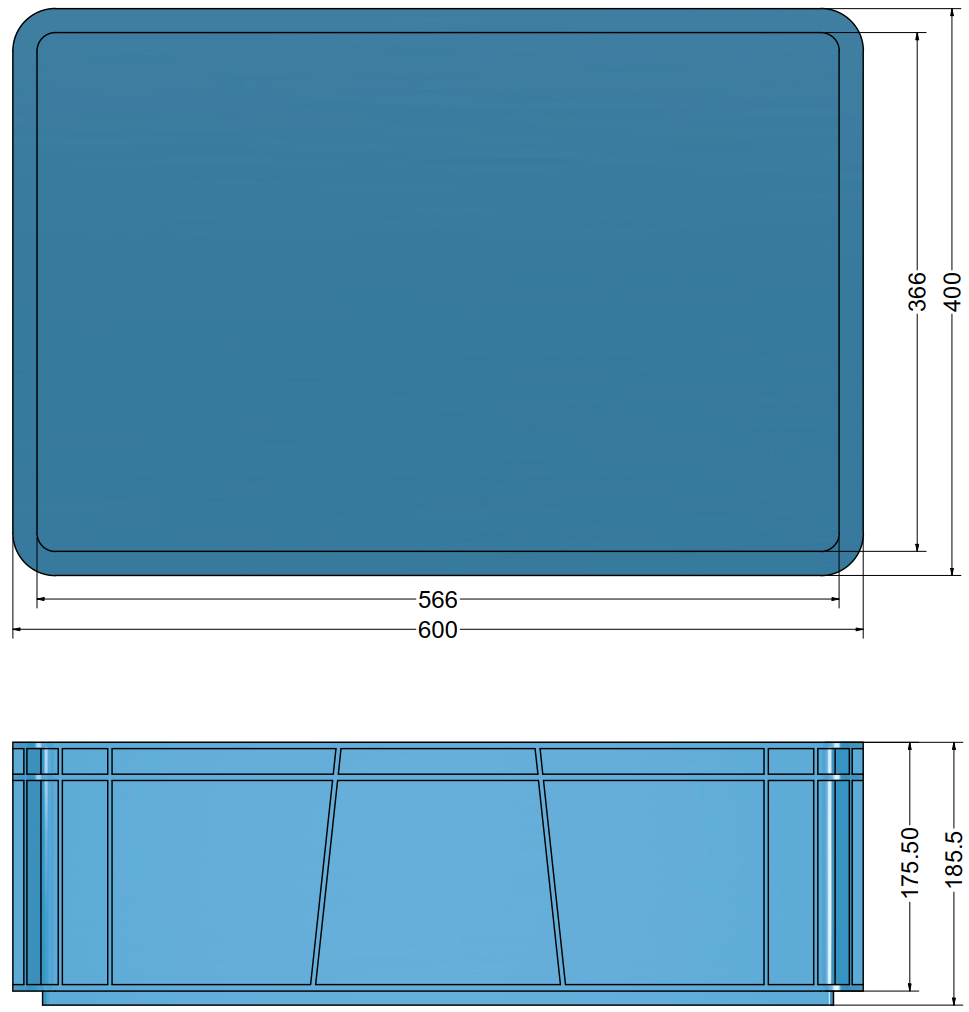
\includegraphics[width=0.9\textwidth]{06disenoConceptual/img/carcasa.png}
        \caption{Vista superior y lateral de canastilla 3/4 sellada con dimensiones externas e internas.}
        \label{fig:carcasa}
    \end{figure}
    
    

\section{Diseño de la Plataforma Base}

\subsection{Dimensionamiento de la Plataforma Base}

Una vez seleccionada la canastilla plástica como contenedor definitivo del kit, se procedió a realizar un levantamiento dimensional completo mediante mediciones directas del producto adquirido. Estas mediciones permitieron establecer las restricciones geométricas que determinarían las dimensiones finales de la plataforma base.

Con el objetivo de maximizar el aprovechamiento del espacio disponible dentro del contenedor, se desarrolló un modelo digital tridimensional de la canastilla que permitió visualizar las restricciones espaciales y planificar la distribución óptima de componentes.

Como se observa en la Figura \ref{fig:carcasa}, la canastilla presenta las siguientes dimensiones:

\begin{itemize}
    \item \textbf{Dimensiones externas}: 600 mm × 400 mm
    \item \textbf{Dimensiones internas útiles}: 566 mm × 366 mm
    \item \textbf{Espesor de pared}: 17 mm (calculado a partir de la diferencia entre dimensiones externas e internas)
\end{itemize}


Considerando las dimensiones internas de la canastilla y la necesidad de dejar holguras mínimas para facilitar el montaje y desmontaje de la plataforma, se establecieron las siguientes dimensiones preliminares para la plataforma base:

\begin{itemize}
    \item \textbf{Ancho de la plataforma}: 365 mm
    \item \textbf{Largo de la plataforma}: 560 mm
\end{itemize}

Estas dimensiones proporcionan:

\begin{itemize}
    \item Holgura lateral: $\frac{566 - 560}{2} = 3$ mm por cada lado en el eje longitudinal
    \item Holgura frontal: $\frac{366 - 365}{2} = 0.5$ mm por cada lado en el eje transversal
\end{itemize}

La selección de estas dimensiones se fundamenta en los siguientes criterios de diseño:

\begin{enumerate}
    \item \textbf{Maximización del espacio útil}: Las dimensiones propuestas aprovechan el 99.3\% del espacio interno disponible en la canastilla (560 mm × 365 mm de 566 mm × 366 mm)
    
    \item \textbf{Tolerancias de ensamblaje}: Las holguras mínimas (0.5 mm - 3 mm) permiten compensar tolerancias dimensionales tanto de la canastilla comercial como de la plataforma a fabricar, facilitando operaciones de montaje y desmontaje
    
    \item \textbf{Compatibilidad con espacio de trabajo del robot}: El largo de 560 mm permite ubicar el robot en posición central con un radio de alcance efectivo de 280 mm, cumpliendo con la restricción de 28.3 cm establecida previamente
    
    \item \textbf{Distribución de zonas funcionales}: El ancho de 365 mm permite distribuir adecuadamente las zonas de recolección, depósito y electrónica a lo largo de la plataforma
\end{enumerate}

Estas dimensiones preliminares serán validadas mediante modelado 3D completo del kit, donde se verificará la disposición espacial de todos los componentes (robot, zonas de trabajo, electrónica, sistema de visión) dentro de los límites establecidos. En caso de identificarse interferencias o restricciones adicionales durante el proceso de diseño detallado, las dimensiones podrán ser ajustadas manteniendo el criterio de máximo aprovechamiento del espacio disponible.


\subsection{Primera Iteración del Diseño de la Plataforma}

\subsubsection{Concepto de Diseño Modular}

Para la primera iteración del diseño de la plataforma, se desarrolló un concepto basado en modularidad y reconfigurabilidad. El objetivo principal fue crear un sistema flexible que permitiera reposicionar las zonas de recolección y depósito según las necesidades didácticas del kit, facilitando diferentes configuraciones experimentales para los estudiantes.

El diseño inicial se fundamentó en una distribución tipo layout que buscaba ubicar los distintos componentes del kit sobre la plataforma base. La estrategia de modularidad se implementó mediante un sistema de celdas cuadradas equipadas con imanes de neodimio, los cuales permitirían el anclaje y reconfiguración de las zonas funcionales sin necesidad de herramientas.

\subsubsection{Componentes del Diseño Inicial}

El modelo 3D de la primera versión del kit comprendía los siguientes componentes, cuyas especificaciones detalladas se presentarán en las secciones correspondientes a cada elemento:

\begin{enumerate}
    \item \textbf{Plataforma base}: Superficie principal de montaje fabricada en MDF de 9 mm de espesor
    
    \item \textbf{Módulos cuadrados}: 18 unidades, cada una equipada con 4 imanes de neodimio en su interior para permitir el anclaje de componentes
    
    \item \textbf{Módulos rectangulares}: 12 unidades, cada una con 2 imanes de neodimio integrados
    
    \item \textbf{Zonas de recolección cuadradas}: 2 unidades, cada una equipada con 16 imanes de neodimio para asegurar su fijación a la plataforma
    
    \item \textbf{Zonas de depósito tipo caneca}: Dos tipos diferenciados por tamaño
    \begin{itemize}
        \item 2 canecas grandes, cada una con 7 imanes de neodimio
        \item 3 canecas pequeñas, cada una con 4 imanes de neodimio
        \item Todas las canecas equipadas con tapas de bisagra para contener objetos durante el transporte del kit
    \end{itemize}
    
    \item \textbf{Soporte de cámara}: Estructura vertical con espacio de anclaje dedicado en la plataforma
    
    \item \textbf{Base del manipulador}: Área de montaje específica para el robot PhantomX Pincher
\end{enumerate}

La Figura \ref{fig:primerDiseñoConceptualKit} presenta el ensamble completo de la plataforma con todos sus componentes integrados, donde se identifican los elementos mediante numeración:

\begin{figure}[H]
    \centering
    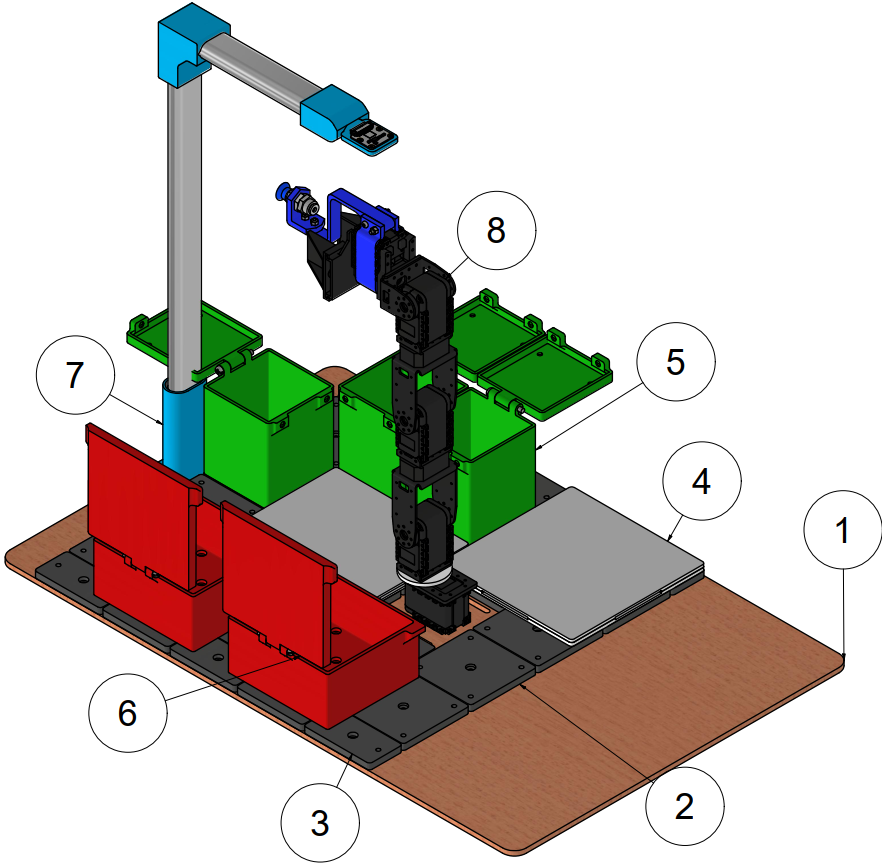
\includegraphics[width=0.9\textwidth]{06disenoConceptual/img/plataforma/ensambleKitObsoleto.png}
    \caption{Primera iteración del diseño conceptual del kit. (1) Plataforma base, (2) Módulo cuadrado, (3) Módulo rectangular, (4) Zona de recolección cuadrada, (5) Caneca pequeña, (6) Caneca grande, (7) Soporte de cámara, (8) Brazo robótico o manipulador}
    \label{fig:primerDiseñoConceptualKit}
\end{figure}

\subsubsection{Desarrollo del Layout de la Plataforma}

El proceso de diseño del layout se desarrolló en dos etapas iterativas:

\paragraph{Layout Inicial - Definición del Área de Trabajo}

El primer layout (Figura \ref{fig:layout1O}) se basó en la restricción cinemática fundamental del manipulador: su alcance efectivo de 283 mm. Se inscribió un cuadrado dentro del círculo formado por dicho alcance, estableciendo así el área de trabajo primaria donde el robot podría operar con máxima libertad de movimiento.

\begin{figure}[H]
    \centering
    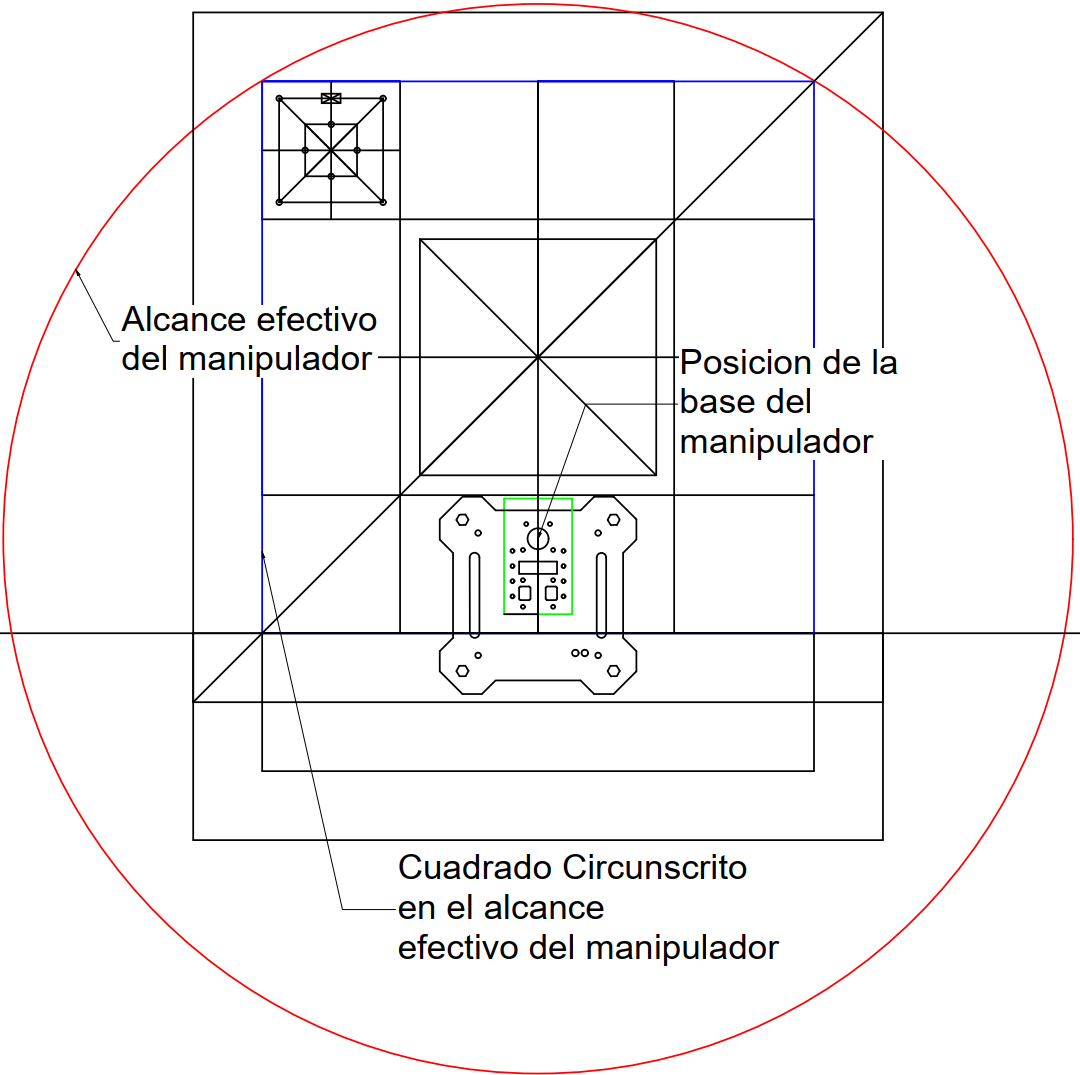
\includegraphics[width=0.7\textwidth]{06disenoConceptual/img/plataforma/layout1Obsoleto.png}
    \caption{Layout inicial de la plataforma mostrando el cuadrado circunscrito en el área de alcance efectivo del manipulador (radio de 283 mm). Se indica la posición central de la base del manipulador.}
    \label{fig:layout1O}
\end{figure}

\paragraph{Layout Refinado - Sistema de Cuadrícula Modular}

A partir del cuadrado de trabajo definido, se desarrolló un sistema de cuadrícula que sirvió como base dimensional para los módulos cuadrados y rectangulares. En esta segunda iteración del layout (Figura \ref{fig:layout2Obsoleto}), se incorporaron elementos adicionales como:

\begin{itemize}
    \item Ubicación del soporte de cámara en posición superior central
    \item Sistema de anclaje mediante orificios roscados para módulos cuadrados
    \item Sistema de anclaje para módulos rectangulares
    \item Puntos de fijación para canecas de depósito
    \item Zona de montaje de la base del manipulador
\end{itemize}

\begin{figure}[H]
    \centering
    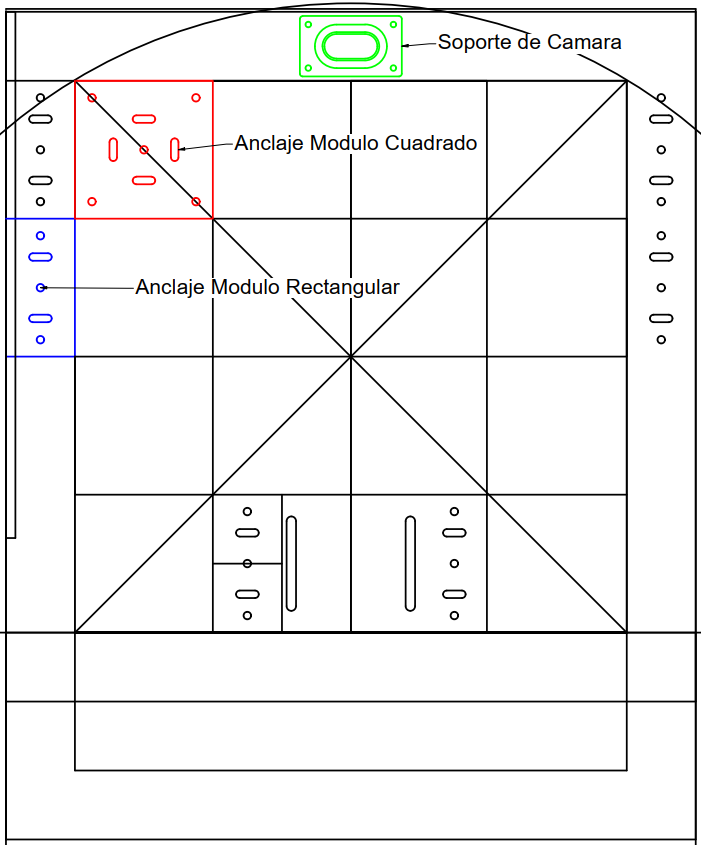
\includegraphics[width=0.7\textwidth]{06disenoConceptual/img/plataforma/layout2obsoleto.png}
    \caption{Layout refinado de la plataforma mostrando el sistema de cuadrícula modular. Se identifican los puntos de anclaje para módulos cuadrados (color rojo) y módulos rectangulares (color azul), así como la ubicación del soporte de cámara en la zona superior.}
    \label{fig:layout2Obsoleto}
\end{figure}


Finalmente se repite el patrón en la cuadricula y se obtiene el modelo 3D de la plataforma inicial que se ve en la figura \ref{fig:plataformaBaseV1.0}

\begin{figure}[H]
    \centering
    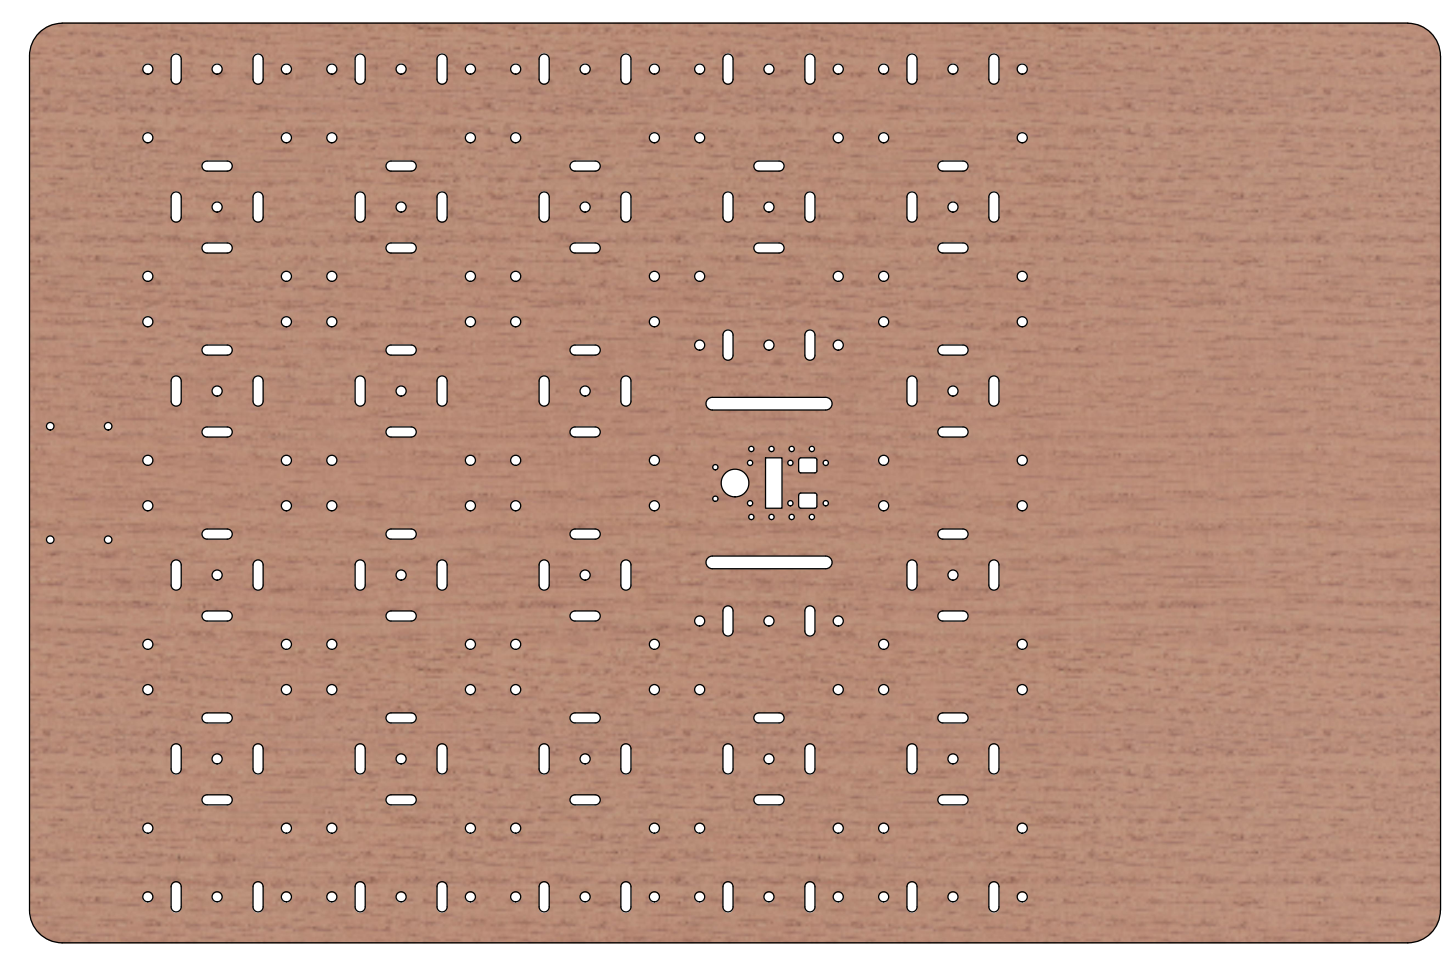
\includegraphics[width=0.7\textwidth]{06disenoConceptual/img/plataforma/plataformaBaseObsoleto.png}
    \caption{ Plataforma base version 1.}
    \label{fig:plataformaBaseV1.0}
\end{figure}

\subsubsection{Selección del Material de la Plataforma}

Para la fabricación de la plataforma base se seleccionó tablero de fibra de densidad media (MDF) de 9 mm de espesor. Esta decisión se fundamentó en un análisis comparativo de costos con materiales alternativos.

Si bien el MDF requiere un proceso de acabado superficial que incluye lijado, sellado, pintado y lacado para garantizar durabilidad y resistencia a la humedad, su relación costo-beneficio resultó significativamente superior a otras opciones consideradas.

\begin{table}[H]
\centering
\caption{Comparación de costos de materiales para la plataforma base}
\label{tab:costos_plataforma}
\begin{tabular}{|l|r|r|}
\hline
\textbf{Material} & \textbf{Costo por unidad} & \textbf{Relación de costo} \\
\hline
MDF 9 mm + corte láser & \$25,000 COP & 1.0× (referencia) \\
Acrílico 9 mm + corte láser & \$200,000 COP & 8.0× \\
\hline
\end{tabular}
\end{table}

El acrílico, a pesar de ofrecer ventajas en términos de resistencia a la humedad y acabado superficial, presentó un costo 8 veces superior al MDF. Considerando que se deben fabricar 7 plataformas (una por cada kit), la diferencia total ascendería a \$1,225,000 COP (\$175,000 en MDF vs \$1,400,000 en acrílico), lo cual excede significativamente el presupuesto disponible por kit.

\subsubsection{Problemas Identificados y Rechazo del Diseño}

A pesar del esfuerzo de diseño invertido, esta primera iteración fue rechazada debido a múltiples deficiencias críticas identificadas durante el proceso de evaluación:

\begin{enumerate}
    \item \textbf{Complejidad excesiva del sistema}: El diseño presentaba un número excesivo de partes móviles e interdependientes, lo cual comprometía la robustez y facilidad de uso del kit. El sistema de 178 imanes de neodimio (distribuidos en módulos, zonas de recolección y canecas) representaba:
    \begin{itemize}
        \item Costo elevado en componentes de fijación
        \item Dificultad en el ensamblaje y mantenimiento
        \item Complejidad innecesaria para los objetivos didácticos del kit
    \end{itemize}
    
    \item \textbf{Dimensionamiento inadecuado de la plataforma}: Las dimensiones de ancho y largo de la plataforma no consideraron las tolerancias de fabricación de la canastilla plástica comercial. Las paredes del contenedor pueden presentar cierta flexión debido a su proceso de moldeo por inyección, lo que dificultaba la extracción e inserción de la plataforma. Las holguras previstas (0.5 mm - 3 mm) resultaron insuficientes en la práctica.
    
    \item \textbf{Error fundamental en el análisis cinemático}: Se cometió un error crítico en el proceso de diseño al no considerar adecuadamente las limitaciones cinemáticas del manipulador. El PhantomX Pincher, al poseer únicamente 4 grados de libertad (DOF), presenta restricciones significativas en su capacidad de orientación del efector final. El uso de una cuadrícula regular como layout asumía implícitamente que el robot podría alcanzar cualquier posición con cualquier orientación, lo cual es cinemáticamente incorrecto para un manipulador de 4 DOF.
    
    Esta limitación implicaba que ciertas celdas de la cuadrícula resultarían inaccesibles o accesibles solo con orientaciones específicas del efector final, comprometiendo la funcionalidad del sistema modular propuesto.
    
    \item \textbf{Ausencia de sistema de manipulación}: No se contempló un método ergonómico y práctico para extraer e insertar la plataforma del contenedor. La ausencia de asas, agarraderas o sistemas de sujeción dificultaba el manejo del kit, especialmente considerando el peso combinado de la plataforma, el robot y los componentes electrónicos.
    
    \item \textbf{Omisión del subsistema electrónico}: El diseño no incluyó una ubicación dedicada para los componentes electrónicos del sistema (controlador, fuente de alimentación, cableado). Esta omisión representaba un problema fundamental, ya que la electrónica constituye un elemento esencial del kit que requiere espacio protegido, ventilación adecuada y accesibilidad para mantenimiento.
\end{enumerate}

\subsubsection{Lecciones Aprendidas}

El proceso de diseño y evaluación crítica de esta primera iteración proporcionó valiosas lecciones que orientaron el desarrollo de versiones subsecuentes:

\begin{itemize}
    \item La modularidad excesiva puede comprometer la funcionalidad y aumentar innecesariamente la complejidad
    \item Las restricciones cinemáticas del manipulador deben ser el punto de partida fundamental del diseño, no una consideración posterior
    \item Las tolerancias de fabricación de componentes comerciales deben verificarse mediante prototipos físicos
    \item El diseño debe considerar todos los subsistemas desde las etapas iniciales (mecánico, electrónico, interfaz de usuario)
    \item La simplicidad y robustez son preferibles a la versatilidad cuando esta última compromete la usabilidad
\end{itemize}

Estas observaciones fundamentaron el desarrollo de una segunda iteración del diseño, la cual se presenta en la siguiente sección.

\subsection{Segunda Iteración del Diseño de la Plataforma}

\subsubsection{Principios de Diseño Revisados}

La segunda iteración del diseño incorporó las lecciones aprendidas del primer prototipo, adoptando un enfoque fundamentalmente diferente basado en los siguientes principios rectores:

\begin{enumerate}
    \item \textbf{Eliminación de la modularidad excesiva}: Las zonas de recolección y depósito se diseñaron como elementos fijos, eliminando el sistema de imanes y módulos intercambiables que añadían complejidad innecesaria
    
    \item \textbf{Simplificación del sistema de clasificación}: Se redujo a una única zona de recolección circular y cuatro zonas de depósito de igual área, simplificando la operación y el software de control
    
    \item \textbf{Integración del subsistema electrónico}: Se incorporó desde el inicio un área dedicada para la Raspberry Pi y una zona flexible para componentes electrónicos adicionales
    
    \item \textbf{Consideración de restricciones cinemáticas}: El posicionamiento de las zonas de trabajo se basó en el análisis del alcance efectivo y las limitaciones de 4 DOF del manipulador
    
    \item \textbf{Mejora de la ergonomía}: Se añadieron manijas para facilitar la manipulación de la plataforma
    
    \item \textbf{Estabilidad y nivelación}: Se incorporaron patas niveladoras en las esquinas y patas de soporte centrales para garantizar estabilidad
    
    \item \textbf{Gestión de cableado}: Se diseñaron canaletas específicas para el paso ordenado de cables
    
    \item \textbf{Sistema de vacío}: Se integró el montaje de la bomba de vacío requerida para el nuevo sistema de sujeción
\end{enumerate}

\subsubsection{Arquitectura de Diseño en Dos Niveles}

A diferencia del diseño anterior, esta iteración requirió considerar la plataforma como un sistema de dos niveles funcionales:

\paragraph{Nivel Superior}
Comprende todos los componentes operativos montados sobre la superficie de la plataforma: zonas de trabajo (recolección y depósito), manipulador, sistema de visión, electrónica de control y sistema de vacío.

\paragraph{Nivel Inferior}
Incluye los elementos estructurales y de servicio ubicados en la cara inferior de la plataforma: sistema de cableado, canaletas, tornillería de fijación, patas niveladoras y estructuras de soporte.

Esta arquitectura de dos niveles permite una separación clara entre funcionalidades operativas y de soporte, facilitando el mantenimiento y modificaciones futuras.

\subsubsection{Análisis de Layouts}

El diseño se desarrolló mediante tres layouts complementarios que abordan diferentes aspectos del sistema:

\paragraph{Layout 1: Análisis Cinemático de Zonas de Depósito}

El primer layout (Figura \ref{fig:layout1}) se centra en la validación cinemática de la ubicación de las zonas de depósito. Este análisis demuestra que todas las zonas de depósito se encuentran dentro del alcance efectivo del robot (círculo rojo con radio de 283 mm).

\begin{figure}[H]
    \centering
    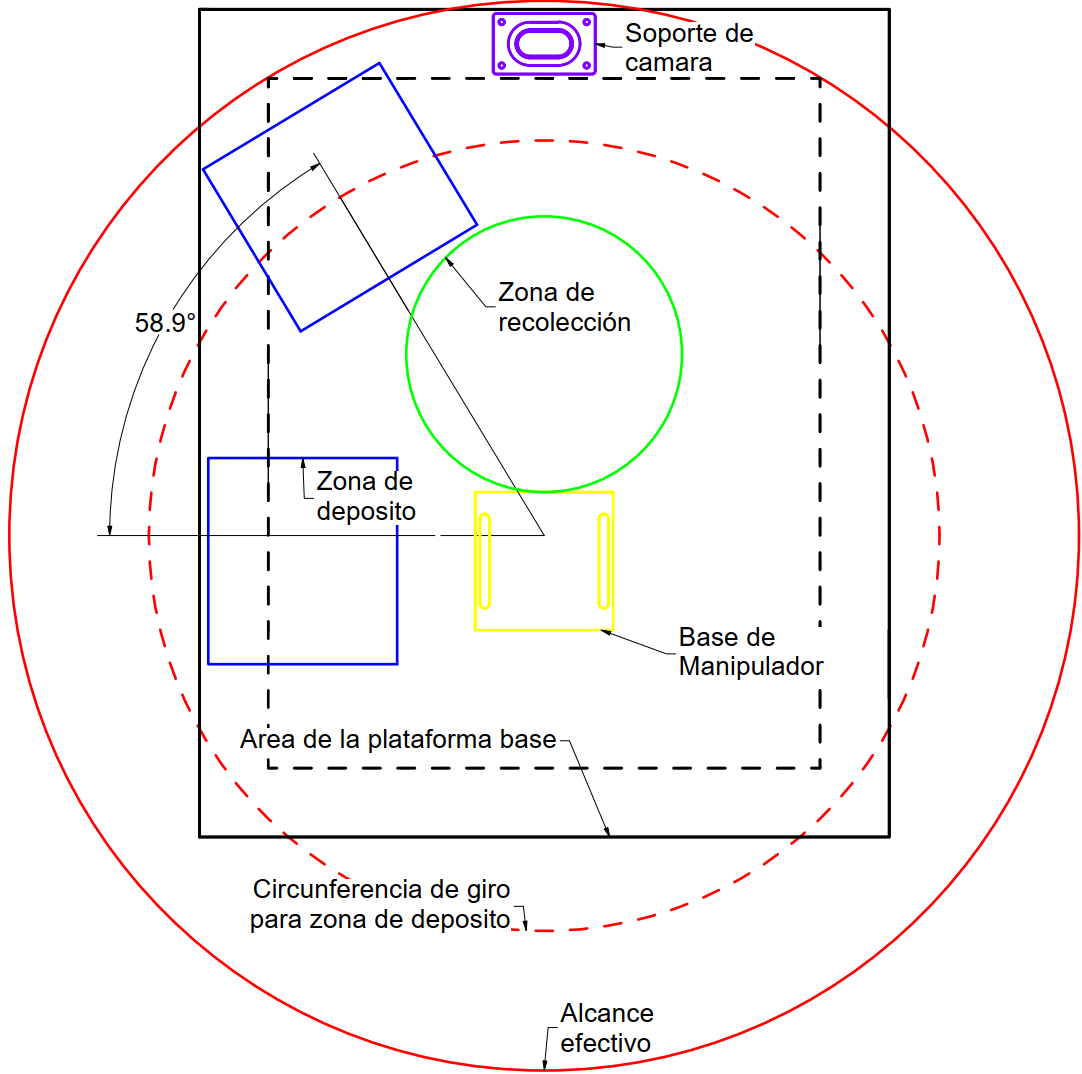
\includegraphics[width=0.75\textwidth]{06disenoConceptual/img/plataforma/layout1.png}
    \caption{Layout 1 - Análisis cinemático de accesibilidad. Se muestra cómo las cuatro zonas de depósito (azul) están contenidas dentro del alcance efectivo del manipulador (círculo rojo). El ángulo de 58.9° indica la rotación angular de las zonas de depósito alrededor del eje de la primera articulación del robot, garantizando accesibilidad desde cualquier configuración. La zona de recolección (verde) se ubica en posición central. Se indica también la circunferencia de giro (línea punteada roja) que delimita el área de trabajo óptima.}
    \label{fig:layout1}
\end{figure}

La estrategia de posicionamiento se basó en la rotación de las zonas de depósito alrededor del eje de la primera articulación (base) del robot. Como se observa en la figura, dos de las zonas de depósito se encuentran rotadas 58.9° con respecto al eje longitudinal de la plataforma. Esta disposición angular garantiza que el manipulador, con sus 4 grados de libertad, pueda alcanzar todas las zonas de depósito mediante rotación de su base y movimientos coordinados de sus eslabones, sin requerir orientaciones imposibles del efector final.

\paragraph{Layout 2: Distribución de Componentes en Nivel Superior}

El segundo layout (Figura \ref{fig:layout2}) presenta la distribución completa de componentes en el nivel superior de la plataforma:

\begin{figure}[H]
    \centering
    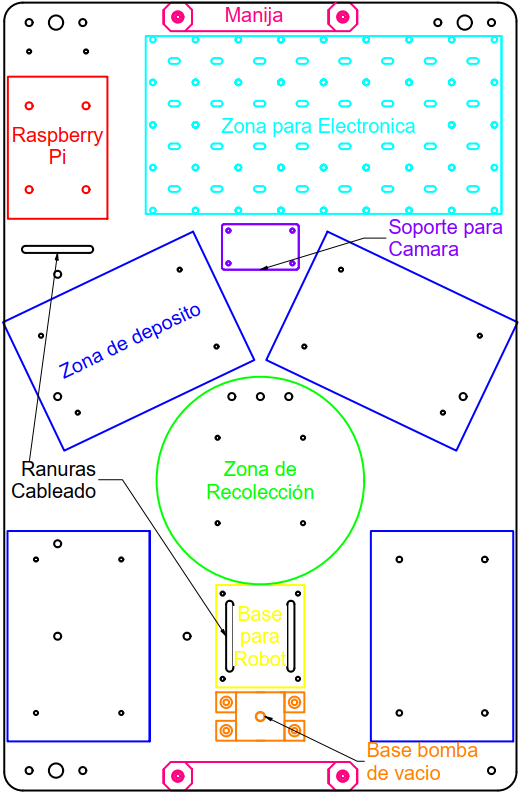
\includegraphics[width=0.75\textwidth]{06disenoConceptual/img/plataforma/layout2.png}
    \caption{Layout 2 - Vista superior de la plataforma mostrando la distribución de todos los componentes operativos. Se identifican: zona de electrónica con retícula de montaje (cian), controlador Raspberry Pi (rojo), cuatro zonas de depósito simétricas (azul), zona de recolección central (verde), base del manipulador (amarillo), soporte de cámara (morado), manijas de transporte (rosa), ranuras de cableado (negro) y base de bomba de vacío (naranja). Las dimensiones corresponden a la plataforma de 560 mm × 365 mm.}
    \label{fig:layout2}
\end{figure}

Los elementos clave identificados en este layout son:

\begin{itemize}
    \item \textbf{Zona de electrónica} (cian): Ubicada en la región posterior, más allá del área de trabajo del robot. Incorpora una retícula de montaje flexible de 30 mm × 30 mm
    \item \textbf{Controlador Raspberry Pi} (rojo): Posición dedicada con montaje específico, ubicada lateralmente para facilitar acceso a puertos
    \item \textbf{Zonas de depósito} (azul): Cuatro receptáculos idénticos distribuidos simétricamente alrededor de la zona de recolección
    \item \textbf{Zona de recolección} (verde): Área circular central donde se posicionan los objetos a clasificar
    \item \textbf{Base del manipulador} (amarillo): Montaje central con patrón de tornillería específico para el PhantomX Pincher
    \item \textbf{Soporte de cámara} (morado): Ubicado entre la zona de electrónica y el área de trabajo, proporcionando vista superior de la escena
    \item \textbf{Manijas de transporte} (rosa): Ubicadas en los bordes superior e inferior de la plataforma para facilitar manipulación
    \item \textbf{Ranuras de cableado} (negro): Aberturas estratégicas para paso de cables entre niveles
    \item \textbf{Base de bomba de vacío} (naranja): Montaje cercano a la base del robot para minimizar longitud de mangueras
\end{itemize}

\paragraph{Layout 3: Componentes del Nivel Inferior}

El tercer layout (Figura \ref{fig:layout3}) detalla los elementos estructurales y de servicio ubicados en el nivel inferior de la plataforma:

\begin{figure}[H]
    \centering
    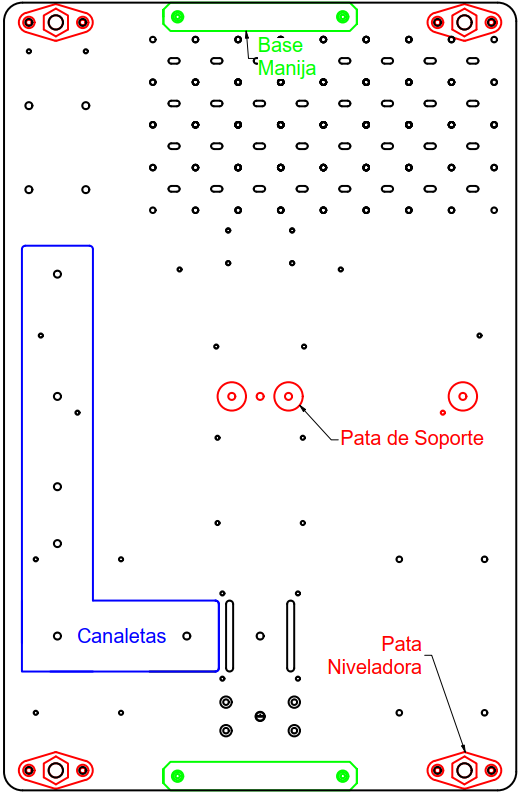
\includegraphics[width=0.75\textwidth]{06disenoConceptual/img/plataforma/layout3.png}
    \caption{Layout 3 - Vista inferior de la plataforma mostrando elementos estructurales y de servicio. Se identifican: canaletas de cableado (azul) en forma de L para gestión ordenada de cables, patas niveladoras (rojo) en las cuatro esquinas con roscas M10, patas de soporte centrales (rojo) para rigidez adicional, manijas de transporte (rosa) con tornillería M6, y base de soporte (verde) para fijación del manipulador. El patrón de agujeros permite la instalación de insertos roscados M4 para montaje de componentes.}
    \label{fig:layout3}
\end{figure}

Los componentes del nivel inferior incluyen:

\begin{itemize}
    \item \textbf{Canaletas de cableado} (azul): Configuración en forma de L que permite el ruteo ordenado de cables desde las zonas de depósito y recolección hacia la zona de electrónica
    \item \textbf{Patas niveladoras} (rojo): Ubicadas en las cuatro esquinas, con agujeros roscados M10 que alojan tornillos de nivelación ajustables
    \item \textbf{Patas de soporte centrales} (rojo): Tres puntos de apoyo adicionales que proporcionan rigidez a la plataforma y evitan flexión en la zona central
    \item \textbf{Manijas} (rosa): Montadas con tornillería M6 que atraviesa completamente la plataforma
    \item \textbf{Patrón de insertos roscados}: Distribución de posiciones para insertos de madera roscados M4 que servirán de anclaje para diversos componentes
\end{itemize}

\subsubsection{Estrategia de Posicionamiento de Zonas Funcionales}

\paragraph{Ubicación de Zonas de Depósito}

El posicionamiento de las zonas de depósito se determinó mediante el siguiente proceso:

\begin{enumerate}
    \item Se trazó el círculo de alcance efectivo del robot (radio de 283 mm) centrado en el eje de su primera articulación
    
    \item Se inscribió un cuadrado dentro de este círculo, similar al enfoque del primer diseño
    
    \item Se posicionó una zona de depósito dentro del cuadrado inscrito
    
    \item Esta zona se rotó alrededor del eje de la primera articulación del robot, generando posiciones angulares múltiples
    
    \item Se seleccionaron cuatro posiciones angulares que maximizaban la separación entre zonas mientras mantenían todas las posiciones dentro del alcance efectivo
\end{enumerate}

Esta estrategia garantiza que el manipulador puede alcanzar cualquier zona de depósito mediante una simple rotación de su base, seguida de movimientos coordinados de sus eslabones. La configuración angular de 58.9° entre zonas adyacentes permite una distribución simétrica que facilita la programación del sistema de control.

\paragraph{Zona de Recolección}

La zona de recolección se diseñó como un área circular ubicada en la región central, delimitada por:

\begin{itemize}
    \item Límite interno: Perímetro de la base del brazo robótico
    \item Límite externo: Circunferencia que conecta las zonas de depósito
\end{itemize}

Esta configuración garantiza que cualquier objeto colocado en la zona de recolección es accesible para el manipulador sin interferencias con su propia base o con las zonas de depósito.

\paragraph{Zona de Electrónica}

La zona de electrónica se ubicó estratégicamente más allá del cuadrado circunscrito en el círculo de alcance máximo del robot. Esta ubicación ofrece múltiples ventajas:

\begin{itemize}
    \item Protección física: Los componentes electrónicos quedan fuera del área de movimiento del manipulador, eliminando riesgo de colisiones
    \item Accesibilidad: Posición en el borde de la plataforma facilita conexión y desconexión de cables
    \item Ventilación: Ubicación alejada de componentes mecánicos permite mejor circulación de aire
    \item Expansibilidad: Área suficiente para añadir componentes adicionales según evolucionen los requerimientos
\end{itemize}

\subsubsection{Sistema de Retícula para Montaje Flexible}

La zona de electrónica incorpora un sistema de retícula que proporciona flexibilidad para cambios futuros en los componentes electrónicos del sistema. Esta retícula se compone de:

\paragraph{Patrón de Agujeros Circulares}
Agujeros pasantes de diámetro apropiado para alojar insertos roscados M4, distribuidos en un patrón rectangular con separación de 30 mm entre centros en ambas direcciones. Este espaciado de 30 mm fue seleccionado por:

\begin{itemize}
    \item Compatibilidad con dimensiones estándar de componentes electrónicos y mecánicos
    \item Suficiente densidad de puntos de fijación sin debilitar excesivamente la estructura de MDF
    \item Coincidencia con múltiplos de dimensiones comunes en sistemas robóticos (15 mm, 60 mm, 90 mm)
\end{itemize}

\paragraph{Ranuras de Cableado}
Ranuras oblongas integradas en el patrón de la retícula que permiten el paso de cables entre componentes montados en la superficie y el nivel inferior de la plataforma. Estas ranuras se encuentran estratégicamente ubicadas para:

\begin{itemize}
    \item Permitir conexiones entre la Raspberry Pi y periféricos
    \item Facilitar el paso de mangueras neumáticas si se requiere posicionar la bomba de vacío en la zona de electrónica (configuración alternativa)
    \item Organizar el cableado de alimentación desde fuentes externas
\end{itemize}

\paragraph{Área Dedicada del Controlador}
Además de la retícula general, se diseñó un área específica para el montaje de la Raspberry Pi, con:

\begin{itemize}
    \item Patrón de agujeros coincidente con los puntos de montaje estándar de la Raspberry Pi
    \item Ranuras adyacentes para paso de cables USB, HDMI, y alimentación
    \item Espacio perimetral para acceso a puertos laterales sin remover el controlador
\end{itemize}

La filosofía de diseño de la retícula permite que la electrónica del robot pueda ser actualizada o modificada sin necesidad de rediseñar la plataforma completa, facilitando la evolución del kit según nuevas necesidades educativas o mejoras tecnológicas.

\subsubsection{Sistemas de Fijación y Anclaje}

El diseño contempla múltiples sistemas de anclaje diferenciados según los requerimientos de carga, frecuencia de desmontaje, y tipo de componente:

\paragraph{Anclajes con Insertos Roscados de Madera M4}

Se seleccionaron insertos roscados de madera M4 como sistema de fijación principal para componentes que requieren desmontaje ocasional. Estos insertos se utilizan en:

\begin{itemize}
    \item Soporte de cámara: 4 puntos de fijación
    \item Patas niveladoras: 4 unidades en las esquinas
    \item Patas de soporte central: 3 unidades
    \item Anclaje de bomba de vacío: Configuración según modelo específico
    \item Carcasa del controlador (Raspberry Pi): 4 puntos de montaje
    \item Zonas de recolección: 4 tornillos de fijación
    \item Zonas de depósito: 4 tornillos de fijación cada una (16 tornillos totales)
    \item Base del robot: 4 tornillos de fijación
\end{itemize}

La selección de insertos roscados de madera sobre alternativas convencionales se fundamentó en:

\begin{enumerate}
    \item \textbf{Durabilidad de la rosca}: Los insertos metálicos proporcionan roscas duraderas que no se degradan con ciclos repetidos de montaje/desmontaje, a diferencia de roscas directas en MDF que se desgastan rápidamente
    
    \item \textbf{Facilidad de reemplazo}: Los componentes pueden ser removidos y reinstalados múltiples veces utilizando tornillos estándar M4, sin deterioro del punto de fijación
    
    \item \textbf{Eliminación de tuercas convencionales}: Se evita el uso de tuercas tradicionales que presentan dos problemas principales:
    \begin{itemize}
        \item Susceptibilidad a caerse o perderse durante operaciones de mantenimiento
        \item Tendencia a dañar el acabado superficial (pintura) de la plataforma debido a la presión de apriete concentrada
    \end{itemize}
    
    \item \textbf{Capacidad de carga}: Los insertos M4 proporcionan resistencia adecuada para las cargas presentes en el sistema (peso de componentes y cargas operativas)
\end{enumerate}

\paragraph{Anclaje de Manijas con Tornillería M6}

Las manijas de transporte utilizan tornillos M6 que atraviesan completamente el espesor de la plataforma y se fijan mediante tuercas en el lado inferior. Esta configuración no requiere insertos roscados debido a:

\begin{itemize}
    \item Menor frecuencia de desmontaje (las manijas permanecen instaladas permanentemente)
    \item Mayor área de distribución de carga mediante arandelas de respaldo
    \item Ubicación en los bordes de la plataforma donde el acabado superficial es menos crítico
    \item Requerimiento de mayor resistencia mecánica para soportar el peso completo del kit durante el transporte
\end{itemize}

\paragraph{Sistema de Nivelación con Roscas M10}

Las patas niveladoras requieren agujeros roscados M10 de mayor diámetro. Se utilizan tornillos M10 de cabeza hexagonal o perillas de ajuste manual que funcionan como patas ajustables en altura. Este sistema permite:

\begin{itemize}
    \item Compensar irregularidades de las superficies de trabajo
    \item Ajustar la horizontalidad de la plataforma para operación óptima del manipulador
    \item Proporcionar apoyo estable en las cuatro esquinas
    \item Facilitar ajuste sin herramientas (si se utilizan perillas de ajuste)
\end{itemize}

\subsubsection{Consideraciones de Acabado Superficial}

\paragraph{Selección de Color}

Se seleccionó pintura negra mate como acabado superficial de la plataforma base. Esta decisión se fundamentó en consideraciones de visión por computador:

\begin{enumerate}
    \item \textbf{Contraste cromático}: El fondo negro maximiza el contraste con las zonas de trabajo, que típicamente utilizan colores brillantes (rojo, verde, amarillo, azul) para facilitar su identificación visual
    
    \item \textbf{Facilitación de segmentación}: Los algoritmos de visión por computador basados en umbralización de color o segmentación por espacios de color (HSV, LAB) operan más eficientemente cuando existe alto contraste entre objetos de interés y fondo
    
    \item \textbf{Reducción de reflejos}: El acabado mate minimiza reflejos especulares que pueden interferir con la captura de imágenes, especialmente bajo iluminación artificial del laboratorio
    
    \item \textbf{Uniformidad del fondo}: Un fondo homogéneo negro simplifica el pre-procesamiento de imágenes, reduciendo la carga computacional del sistema de visión
\end{enumerate}

\paragraph{Proceso de Acabado del MDF}

El proceso completo de acabado superficial contempla las siguientes etapas:

\begin{enumerate}
    \item \textbf{Lijado inicial}: Lijado con papel de grano 120-150 para eliminar irregularidades del corte láser
    \item \textbf{Sellado}: Aplicación de sellador para MDF que reduce porosidad y mejora adherencia de la pintura
    \item \textbf{Lijado intermedio}: Lijado con grano 220 después del secado del sellador
    \item \textbf{Aplicación de pintura}: 2-3 capas de pintura negra mate, con lijado suave entre capas
    \item \textbf{Lacado}: Capa final de laca mate transparente para protección contra desgaste y humedad
\end{enumerate}

Este proceso de acabado, aunque laborioso, resulta económicamente viable considerando el ahorro sustancial respecto a materiales alternativos como el acrílico.

\subsubsection{Gestión de Cableado}

El sistema de canaletas en el nivel inferior proporciona rutas dedicadas para diferentes tipos de cables:

\begin{itemize}
    \item \textbf{Cables de potencia}: Desde la fuente de alimentación externa hasta la zona de electrónica
    \item \textbf{Cables de control}: Desde la Raspberry Pi hasta el controlador del manipulador
    \item \textbf{Cables de sensores}: Desde las zonas de trabajo hasta el controlador
    \item \textbf{Cables de comunicación}: Conexiones USB, Ethernet, u otros protocolos de comunicación
    \item \textbf{Mangueras neumáticas}: Desde la bomba de vacío hasta el efector final del manipulador
\end{itemize}

La configuración en forma de L de las canaletas permite una distribución eficiente que minimiza cruces de cables y facilita el mantenimiento.

\subsubsection{Diseño Final de la Plataforma Base}

El diseño final de la plataforma base se presenta en la Figura \ref{fig:plataformaBaseVersionFinal}, donde se observan las dimensiones definitivas y la distribución completa de agujeros y ranuras para el montaje de componentes.

\begin{figure}[H]
    \centering
    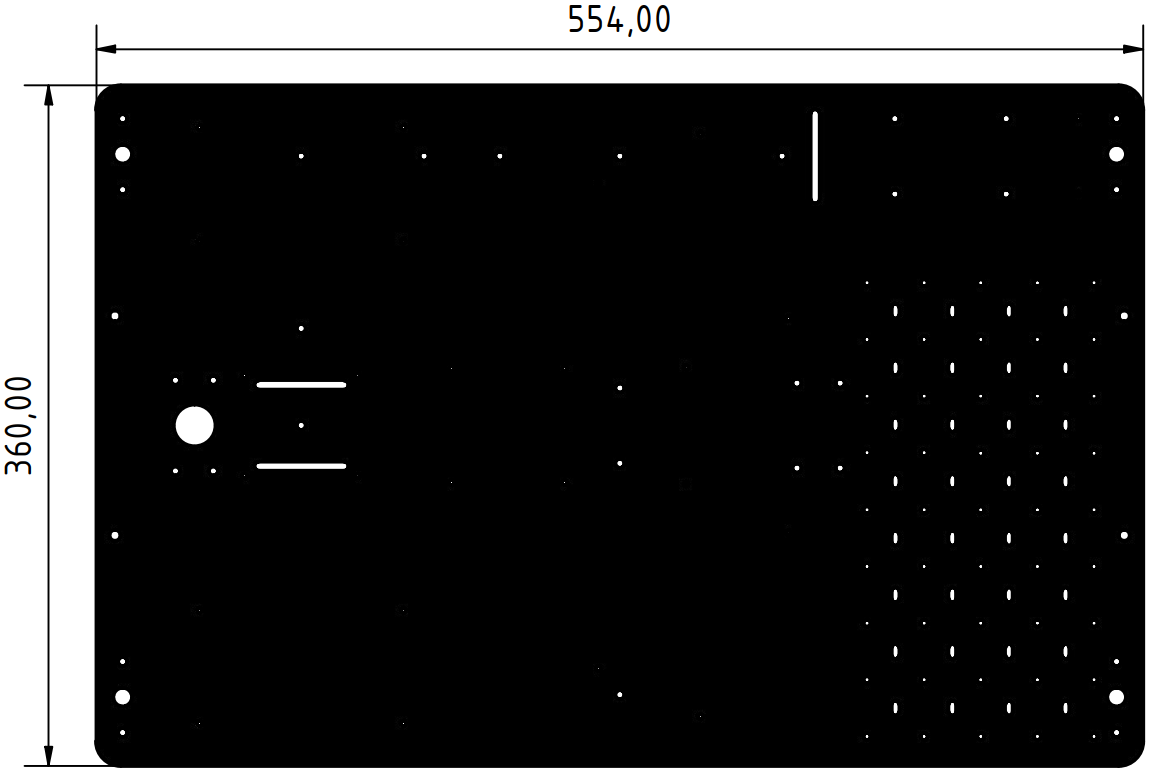
\includegraphics[width=0.95\textwidth]{06disenoConceptual/img/plataforma/baseFijaPlano.png}
    \caption{Plano técnico de la plataforma base con dimensiones finales de 554.00 mm × 360.00 mm. Se muestran los agujeros para insertos roscados M4, agujeros para patas niveladoras M10 en las esquinas, ranuras de cableado y la retícula de montaje en la zona de electrónica. El acabado es negro mate para contraste visual.}
    \label{fig:plataformaBaseVersionFinal}
\end{figure}

Las dimensiones finales de la plataforma son 554 mm de largo por 360 mm de ancho, fabricada en MDF de 9 mm de espesor. Estas dimensiones proporcionan holguras de 6 mm y 3 mm con respecto a las dimensiones internas del contenedor (566 mm × 366 mm), facilitando las operaciones de inserción y extracción de la plataforma.

Todos los elementos geométricos mostrados en el plano (agujeros circulares, ranuras oblongas y el perímetro exterior) son completamente realizables mediante corte láser en una única lámina de MDF. El proceso de corte láser garantiza la precisión dimensional necesaria y permite la fabricación repetible de las 7 plataformas requeridas con tolerancias de ±0.1 mm.

Posterior al corte, cada plataforma se somete al proceso de acabado superficial (lijado, sellado, pintado negro mate y lacado) para garantizar durabilidad y proporcionar el contraste visual necesario para los algoritmos de visión por computador.


\subsection{Componentes Estructurales de la Plataforma Base}

La plataforma base integra diversos componentes estructurales diseñados para proporcionar estabilidad, facilitar el transporte y permitir la gestión ordenada del cableado. A continuación se describen estos componentes y sus especificaciones técnicas.

\subsubsection{Patas Niveladoras}

Las patas niveladoras, mostradas en la Figura \ref{fig:pataNiveladora}, permiten ajustar la horizontalidad de la plataforma para compensar irregularidades en las superficies de trabajo. Cada pata niveladora es un subconjunto compuesto por cuatro elementos:

\begin{figure}[H]
    \centering
    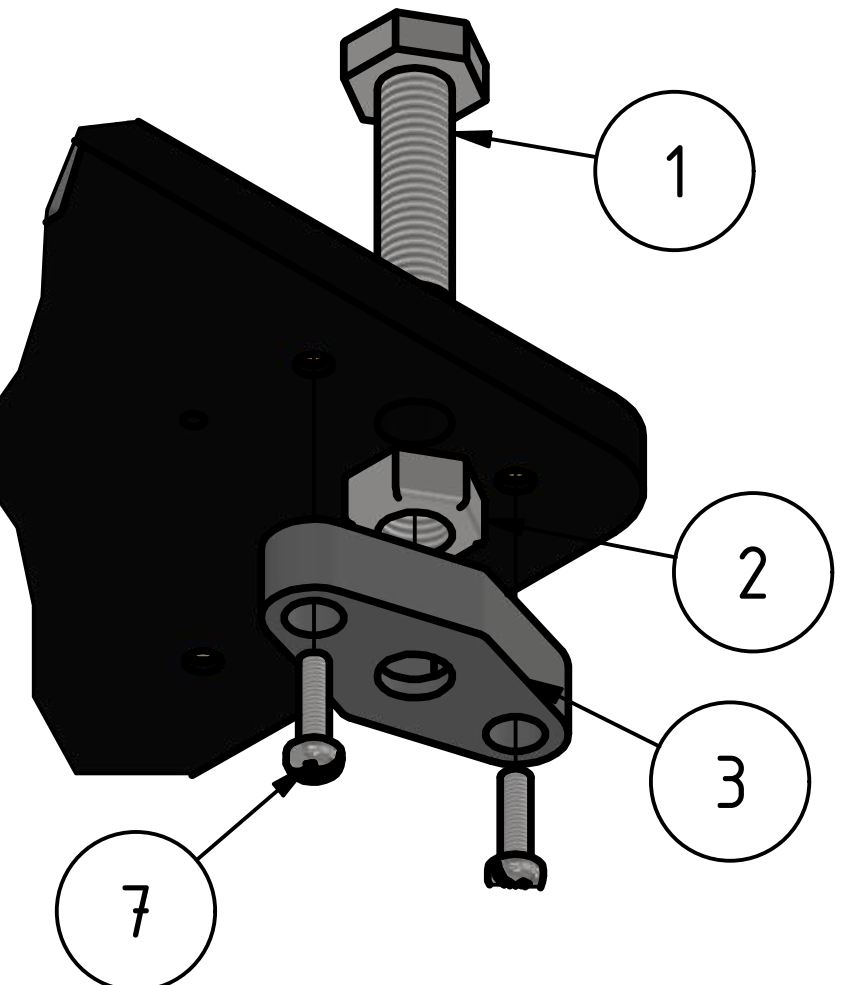
\includegraphics[width=0.5\textwidth]{06disenoConceptual/img/plataforma/pataNiveladora.png}
    \caption{Ensamble de pata niveladora. (1) Tornillo M10 × 35 mm que funciona como elemento de ajuste de altura, (2) Acople impreso en 3D con cavidad hexagonal para alojar la tuerca M10.}
    \label{fig:pataNiveladora}
\end{figure}

\begin{table}[H]
\centering
\caption{Lista de materiales de la pata niveladora}
\label{tab:bom_pata_niveladora}
\small
\begin{tabular}{|c|l|c|l|l|}
\hline
\textbf{\#} & \textbf{Componente} & \textbf{Cant.} & \textbf{Fabricación} & \textbf{Material} \\
\hline
1 & Tornillo M10 × 35 mm & 1 & Comercial & Acero \\
2 & Tuerca M10 & 1 & Comercial & Acero \\
3 & Acople de pata niveladora & 1 & FDM & PLA/ABS \\
4 & Tornillo M4 × 15 mm & 2 & Comercial & Acero \\
\hline
\end{tabular}
\end{table}

El acople de pata niveladora incorpora una cavidad hexagonal que aloja la tuerca M10, impidiendo su rotación. Este acople se fija a la plataforma mediante dos tornillos M4 que se enroscan en insertos roscados ubicados en las esquinas. El tornillo M10 atraviesa la plataforma y el acople, actuando como elemento de ajuste de altura mediante rotación manual.

\subsubsection{Patas de Soporte Central}

Las patas de soporte central (Figura \ref{fig:pataSoporte}) se ubican en la zona media de la plataforma para evitar flexión excesiva cuando se aplican cargas sobre su superficie. Estas patas son especialmente importantes considerando el espesor de 9 mm del MDF y la envergadura de 554 mm de la plataforma.

\begin{figure}[H]
    \centering
    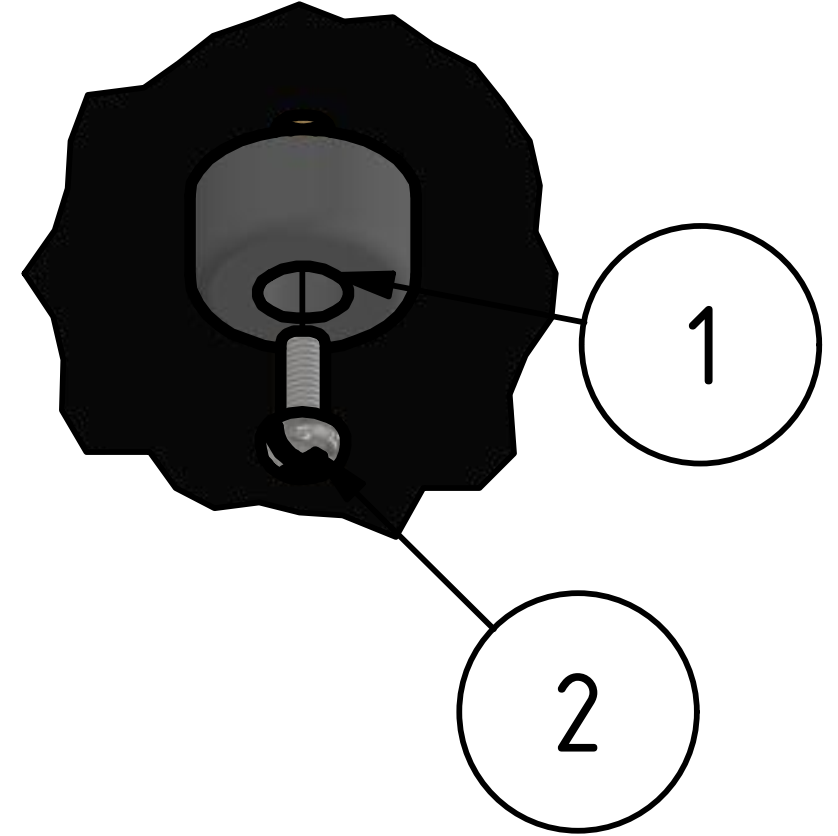
\includegraphics[width=0.45\textwidth]{06disenoConceptual/img/plataforma/pataSoporte.png}
    \caption{Pata de soporte central. (1) Pata fabricada mediante FDM, (2) Vista del montaje en la cara inferior de la plataforma.}
    \label{fig:pataSoporte}
\end{figure}

\begin{table}[H]
\centering
\caption{Lista de materiales de la pata de soporte}
\label{tab:bom_pata_soporte}
\small
\begin{tabular}{|c|l|c|l|l|}
\hline
\textbf{\#} & \textbf{Componente} & \textbf{Cant.} & \textbf{Fabricación} & \textbf{Material} \\
\hline
1 & Pata de soporte & 1 & FDM & ABS/PLA \\
2 & Tornillo M4 × 10 mm & 1 & Comercial & Acero \\
\hline
\end{tabular}
\end{table}

Cada pata se fija mediante un tornillo M4 que se enrosca en un inserto roscado de la plataforma. Se utilizan tres patas de soporte distribuidas en la zona central para proporcionar rigidez estructural sin interferir con las canaletas de cableado.

\subsubsection{Manijas de Transporte}

Las manijas permiten la manipulación ergonómica de la plataforma completa. Su diseño considera datos antropométricos de la población colombiana para garantizar un agarre cómodo y seguro.

\paragraph{Consideraciones Antropométricas}

Según estudios del Imperial College of London y la Asociación Colombiana de Endocrinología, la estatura promedio en Colombia es de 172.4 cm para hombres y 159.3 cm para mujeres. En cuanto a dimensiones de la mano, el ancho de palma es de aproximadamente 8.9 cm para hombres y 7.9 cm para mujeres, mientras que el grosor de los dedos oscila entre 15-20 mm según datos antropométricos internacionales ajustados a la población colombiana. \cite{NCDRisC2020} \cite{Binvignat2012} \cite{Rodriguez2024}

Con base en estos datos, se diseñó una abertura de agarre de 96 mm de ancho. Este valor resulta del compromiso entre comodidad ergonómica (que requeriría anchos mayores) y las restricciones espaciales impuestas por las mangueras neumáticas que conectan la bomba de vacío con el manipulador.

\begin{figure}[H]
    \centering
    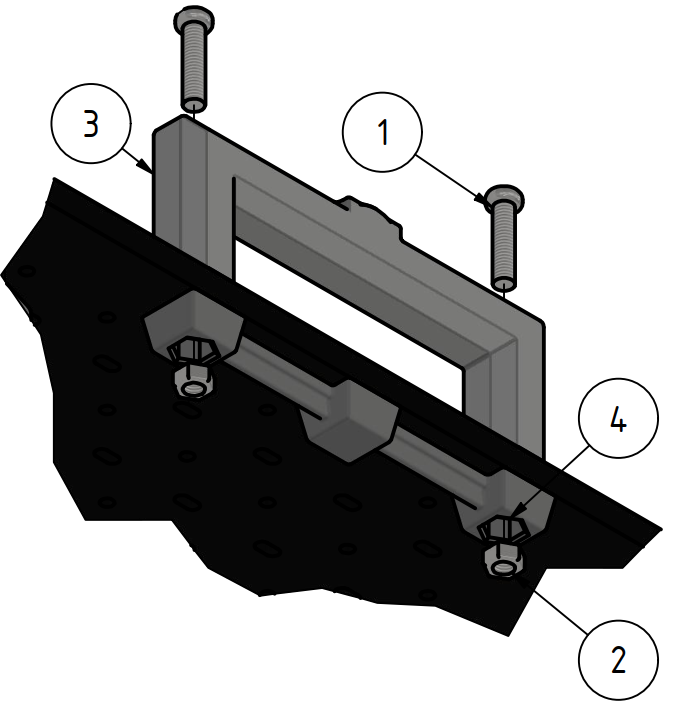
\includegraphics[width=0.6\textwidth]{06disenoConceptual/img/plataforma/manija.png}
    \caption{Ensamble de manija de transporte. (1) Tornillos M6 × 25 mm, (2) Tuercas M6 alojadas en la pata, (3) Cuerpo de la manija (nivel superior), (4) Pata de soporte de la manija (nivel inferior).}
    \label{fig:manija}
\end{figure}

\begin{table}[H]
\centering
\caption{Lista de materiales del subconjunto de manija}
\label{tab:bom_manija}
\small
\begin{tabular}{|c|l|c|l|l|}
\hline
\textbf{\#} & \textbf{Componente} & \textbf{Cant.} & \textbf{Fabricación} & \textbf{Material} \\
\hline
1 & Tornillo M6 × 25 mm & 2 & Comercial & Acero \\
2 & Tuerca M6 & 2 & Comercial & Acero \\
3 & Manija & 1 & FDM & PLA/ABS \\
4 & Pata de manija & 1 & FDM & PLA/ABS \\
\hline
\end{tabular}
\end{table}

El ensamble consta de una manija superior y una pata inferior conectadas mediante dos tornillos M6 que atraviesan completamente la plataforma. Las tuercas M6 se alojan en cavidades de la pata inferior, donde quedan cautivas. La pata cumple una función estructural crítica: proporciona soporte vertical para evitar flexión de la plataforma en caso de que alguien se apoye accidentalmente sobre la manija durante el transporte.

\subsubsection{Sistema de Canaletas}

Las canaletas organizan y protegen el cableado que conecta los diferentes subsistemas del kit. El diseño contempla cuatro canales independientes que permiten el paso de:

\begin{itemize}
    \item Cables de control desde la Raspberry Pi hasta el controlador del manipulador
    \item Cables de alimentación para la bomba de vacío
    \item Manguera neumática de 4 mm de diámetro (configuración actual o futura)
    \item Canal adicional para expansiones futuras
\end{itemize}

\begin{figure}[H]
    \centering
    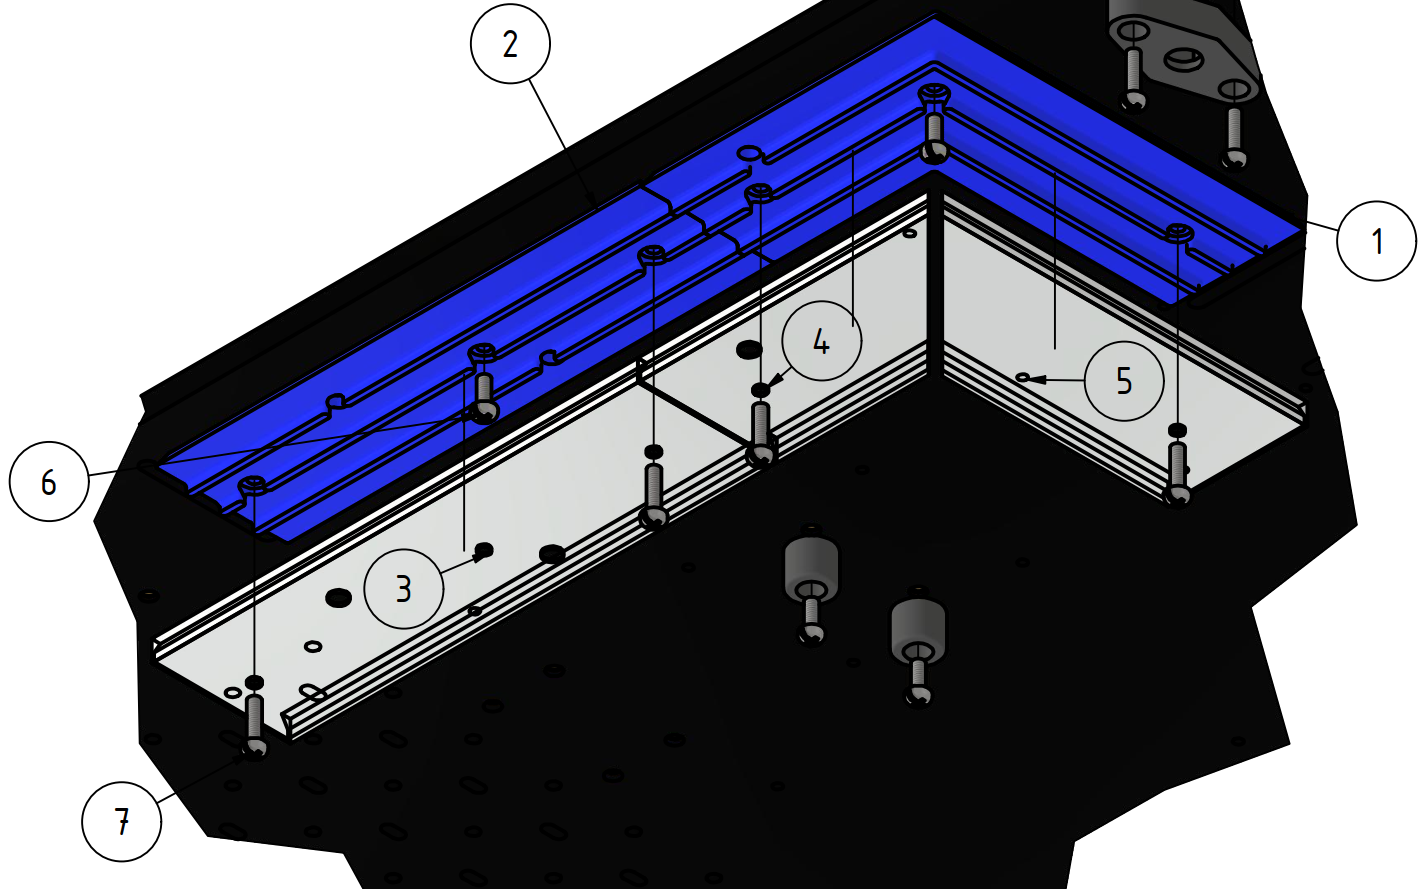
\includegraphics[width=0.8\textwidth]{06disenoConceptual/img/plataforma/canaleta.png}
    \caption{Sistema de canaletas para gestión de cableado. (1) Codo de canaleta, (2) Tapas transparentes en PETG (tres segmentos), (3) Canaleta recta, (4-5) Canales internos para separación de cables, (6) Zona de anclaje con tornillos M4, (7) Tornillos de fijación a insertos roscados de la plataforma.}
    \label{fig:canaleta}
\end{figure}

La canaleta presenta geometría en forma de L, conectando la ranura cercana al controlador con la ranura próxima al manipulador. Debido a las limitaciones del volumen de impresión de las impresoras FDM disponibles, el sistema se divide en dos componentes base:

\begin{itemize}
    \item Codo de canaleta: Sección angular que conecta ambos ejes
    \item Canaleta recta: Segmento longitudinal
\end{itemize}

Las tapas se fabrican en PETG transparente, permitiendo inspección visual del cableado sin necesidad de desmontaje. Esta característica facilita las tareas de mantenimiento y resolución de problemas. La configuración en L de la tapa requiere su división en tres segmentos para viabilizar su fabricación mediante FDM.

\begin{table}[H]
\centering
\caption{Lista de materiales del sistema de canaletas}
\label{tab:bom_canaleta}
\small
\begin{tabular}{|c|l|c|l|l|}
\hline
\textbf{\#} & \textbf{Componente} & \textbf{Cant.} & \textbf{Fabricación} & \textbf{Material} \\
\hline
1 & Codo de canaleta & 1 & FDM & PLA/ABS \\
2 & Canaleta recta & 1 & FDM & PLA/ABS \\
3 & Tapa larga & 1 & FDM & PETG \\
4 & Tapa diagonal 110 mm & 1 & FDM & PETG \\
5 & Tapa diagonal 135 mm & 1 & FDM & PETG \\
6 & Tornillo M4 × 10 mm & 2 & Comercial & Acero \\
7 & Tornillo M4 × 15 mm & 4 & Comercial & Acero \\
\hline
\end{tabular}
\end{table}

El sistema de canaletas se fija a la plataforma mediante tornillos M4 que se enroscan en insertos roscados ubicados estratégicamente en el nivel inferior. Las tapas se deslizan en guías laterales de la canaleta, permitiendo acceso rápido al interior sin necesidad de desmontar completamente el sistema.
\subsection{Diseño de Zonas de Depósito}

Las zonas de depósito constituyen los receptáculos donde el manipulador deposita los objetos clasificados. El diseño de estos componentes evolucionó a través de un proceso iterativo que permitió identificar y resolver múltiples deficiencias del concepto inicial.

\subsubsection{Primera Iteración: Canecas con Sistema de Imanes}

El diseño inicial contemplaba dos tipos de canecas de diferentes tamaños (Figura \ref{fig:canecasIman}): canecas grandes para objetos voluminosos y canecas pequeñas para objetos de menor tamaño. Ambos tipos incorporaban imanes de neodimio en su base para acoplarse a los módulos cuadrados y rectangulares de la primera iteración de la plataforma base.

\begin{figure}[H]
    \centering
    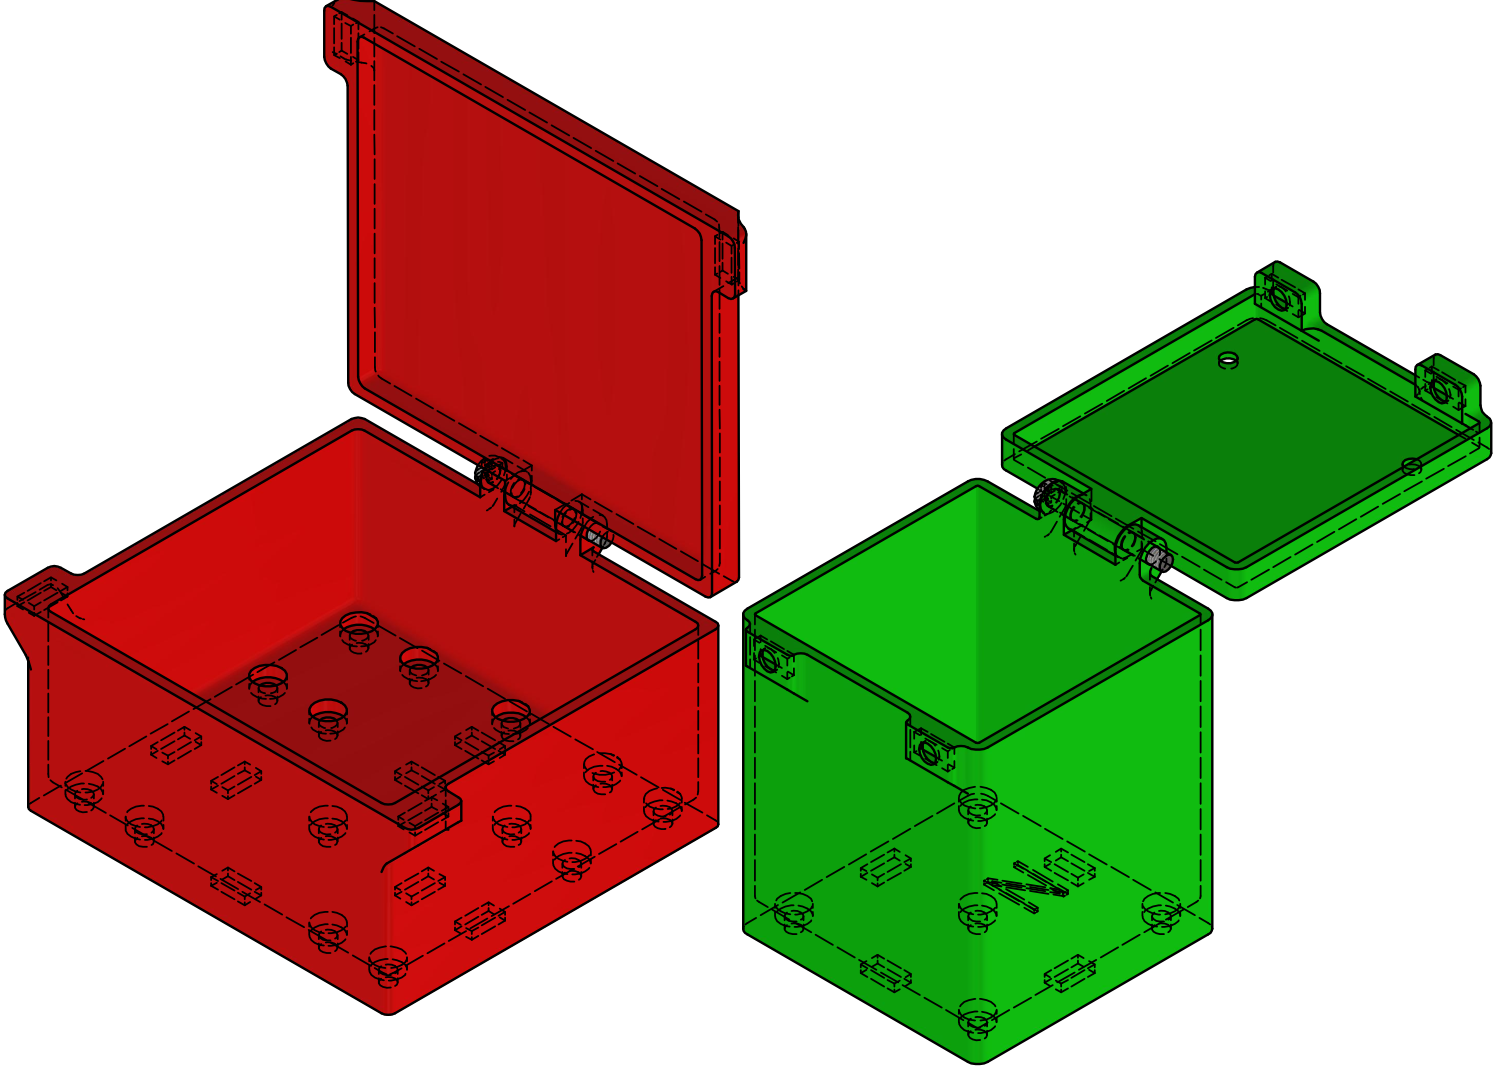
\includegraphics[width=0.7\textwidth]{06disenoConceptual/img/canecas/canecasIman.png}
    \caption{Primera iteración del diseño de zonas de depósito. Se muestran dos tipos de canecas (grande en rojo y pequeña en verde) equipadas con imanes de neodimio en su base y tapas abatibles por bisagra. Ambos diseños incluyen cavidades para alojar imanes y agujeros roscados para fijación opcional a la plataforma.}
    \label{fig:canecasIman}
\end{figure}

Estas canecas incluían tapas con bisagra y agujeros para anclaje permanente opcional a la plataforma. Sin embargo, este diseño fue descartado completamente debido a las siguientes deficiencias críticas:

\begin{enumerate}
    \item \textbf{Dependencia de imanes}: El sistema de fijación basado en atracción magnética resultó insuficientemente robusto para garantizar estabilidad durante las operaciones de depósito y transporte
    
    \item \textbf{Interferencia visual}: Los agujeros de tornillería visibles en la superficie superior comprometían los algoritmos de visión por computador, dificultando la discriminación entre objetos de interés y elementos estructurales (cabezas de tornillos)
    
    \item \textbf{Restricción de accesibilidad}: Las dimensiones de apertura no permitían la entrada de la garra del robot, limitando la funcionalidad exclusivamente a depósito y eliminando la posibilidad de recolección desde las canecas
    
    \item \textbf{Complejidad innecesaria}: El diseño requería múltiples tipos de elementos de fijación (tornillos, tuercas, imanes) aumentando costo y dificultad de ensamblaje
    
    \item \textbf{Aprovechamiento ineficiente del espacio}: El mecanismo de cierre por bisagra generaba volumen muerto en la parte superior de las canecas
\end{enumerate}

\subsubsection{Especificación de Requerimientos para el Rediseño}

A partir de las deficiencias identificadas, se establecieron los siguientes requerimientos para las iteraciones subsecuentes:

\begin{itemize}
    \item La garra del PhantomX Pincher debe poder acceder al interior de las canecas, tanto para depósito como para eventual recolección de objetos
    \item Geometría simple sin artefactos visuales que puedan interferir con los algoritmos de visión por computador
    \item Reducción del número de componentes y simplificación del ensamblaje
    \item Estandarización en un único tipo de caneca para todas las zonas de depósito
    \item Sistema de fijación permanente a la plataforma base
    \item Conservación de sistema de cierre para contención de objetos durante transporte
\end{itemize}

\subsubsection{Análisis Dimensional para Accesibilidad de Garras}

El dimensionamiento de las canecas consideró la compatibilidad con dos variantes del robot PhantomX Pincher disponibles en el laboratorio:

\paragraph{PhantomX Pincher AX-12}
La garra de esta variante (Figura \ref{fig:garraPXP-AX12}) presenta dimensiones de aproximadamente 72 mm de ancho por 61 mm de alto.

\begin{figure}[H]
    \centering
    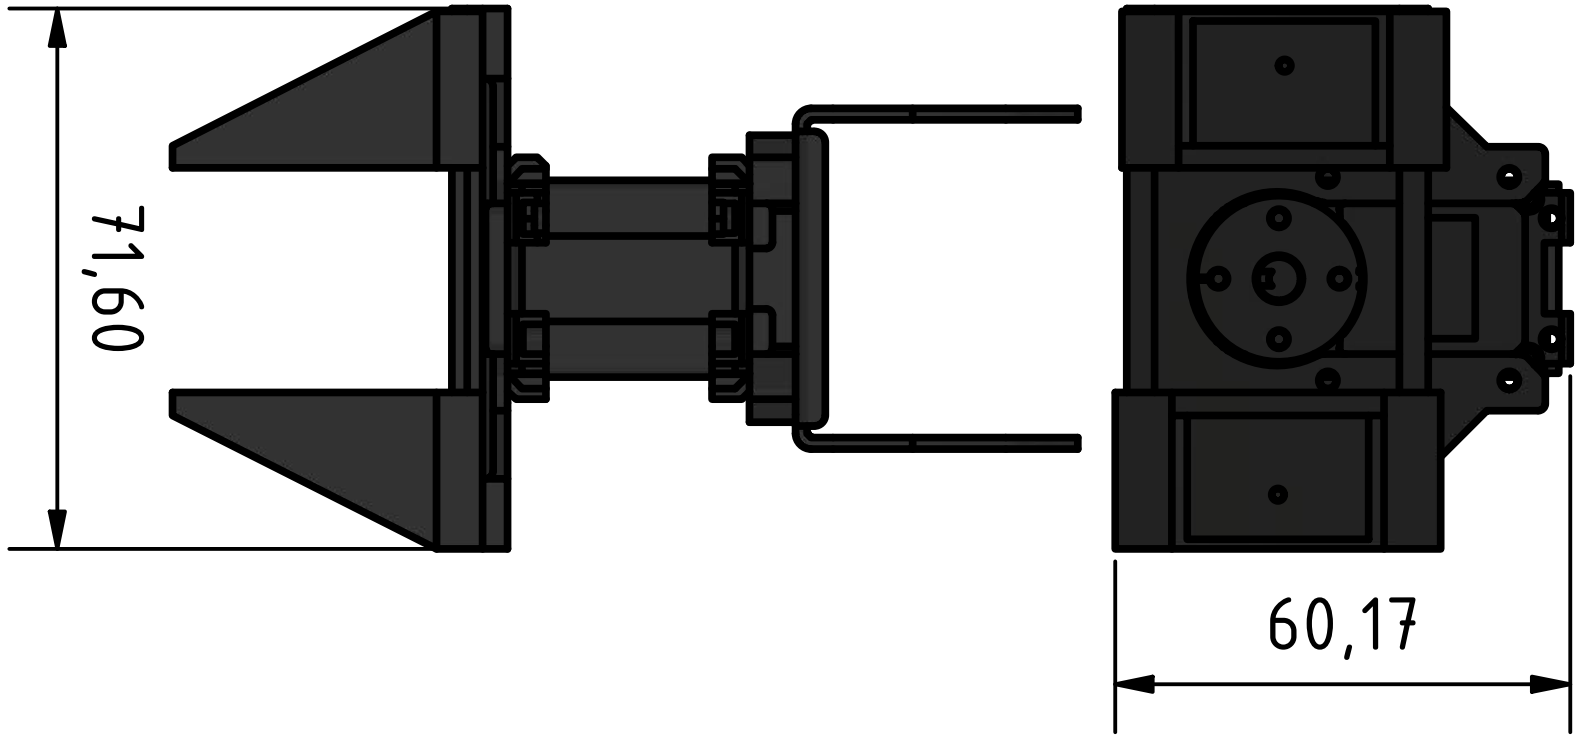
\includegraphics[width=0.5\textwidth]{06disenoConceptual/img/canecas/garraPXP-AX12.png}
    \caption{Garra del robot PhantomX Pincher AX-12. Dimensiones: 72 mm de ancho × 61 mm de alto. Se observan los dedos de la garra (cian) y el servomotor Dynamixel AX-12A (rosa) que controla la apertura/cierre.}
    \label{fig:garraPXP-AX12}
\end{figure}

\paragraph{PhantomX Pincher A100}
La garra de esta variante (Figura \ref{fig:garraPXA100}) posee dimensiones mayores: 104 mm de ancho por 54 mm de alto aproximadamente.

\begin{figure}[H]
    \centering
    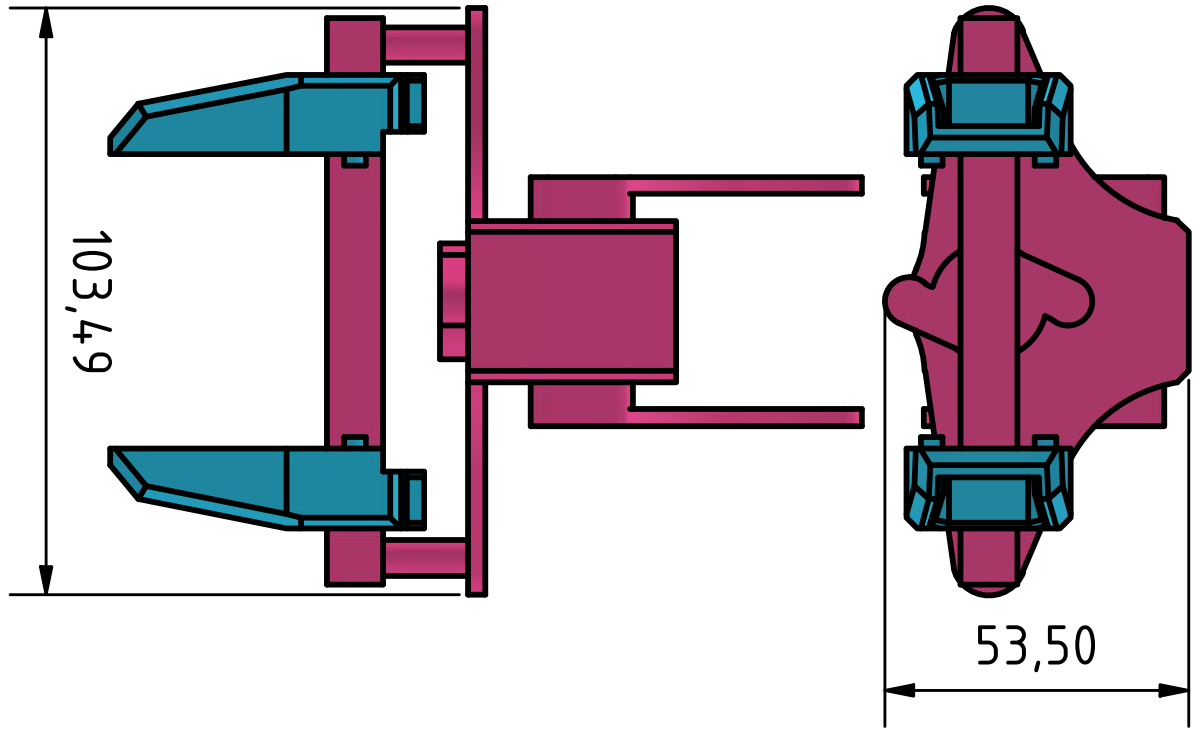
\includegraphics[width=0.5\textwidth]{06disenoConceptual/img/canecas/garraPXA100.png}
    \caption{Garra del robot PhantomX Pincher A100. Dimensiones: 104 mm de ancho × 54 mm de alto. Esta variante presenta mayor apertura máxima que el modelo AX-12.}
    \label{fig:garraPXA100}
\end{figure}

\subsubsection{Diseño Final de las Canecas}

El diseño definitivo de las canecas se desarrolló considerando las restricciones cinemáticas, espaciales y de manufactura identificadas durante el proceso de diseño de la plataforma.

\paragraph{Dimensionamiento Longitudinal}

El largo de las canecas se determinó a partir del ángulo de rotación de 58.9° de las zonas de depósito visible en los layouts de las Figuras \ref{fig:layout1} y \ref{fig:layout2}. Partiendo de este ángulo, se maximizó la dimensión longitudinal sin invadir áreas asignadas a otros componentes, resultando en un ancho exterior de 148 mm y un ancho interior útil de 142 mm.

\paragraph{Apertura Frontal}

Se incorporó una apertura frontal de 131 mm de ancho que permite el acceso de la garra por el frente de la caneca. Esta dimensión proporciona holguras laterales de:
\begin{itemize}
    \item 29 mm por lado para la garra AX-12 (ancho 72 mm)
    \item 13 mm por lado para la garra A100 (ancho 104 mm)
\end{itemize}

Estas holguras son suficientes para permitir el ingreso de las garras considerando tolerancias de posicionamiento del manipulador.

\paragraph{Sistema de Tapa Deslizante}

En la parte inferior de la apertura frontal se incorporó un chaflán de 45° que define una guía para una tapa deslizante. Este diseño ofrece ventajas significativas sobre el sistema de bisagra del diseño anterior:

\begin{itemize}
    \item La tapa no puede ser desplazada verticalmente, permaneciendo cautiva durante el transporte
    \item El movimiento únicamente horizontal facilita las operaciones de cierre
    \item Se elimina el volumen muerto superior presente en el diseño con bisagra
\end{itemize}

\begin{figure}[H]
    \centering
    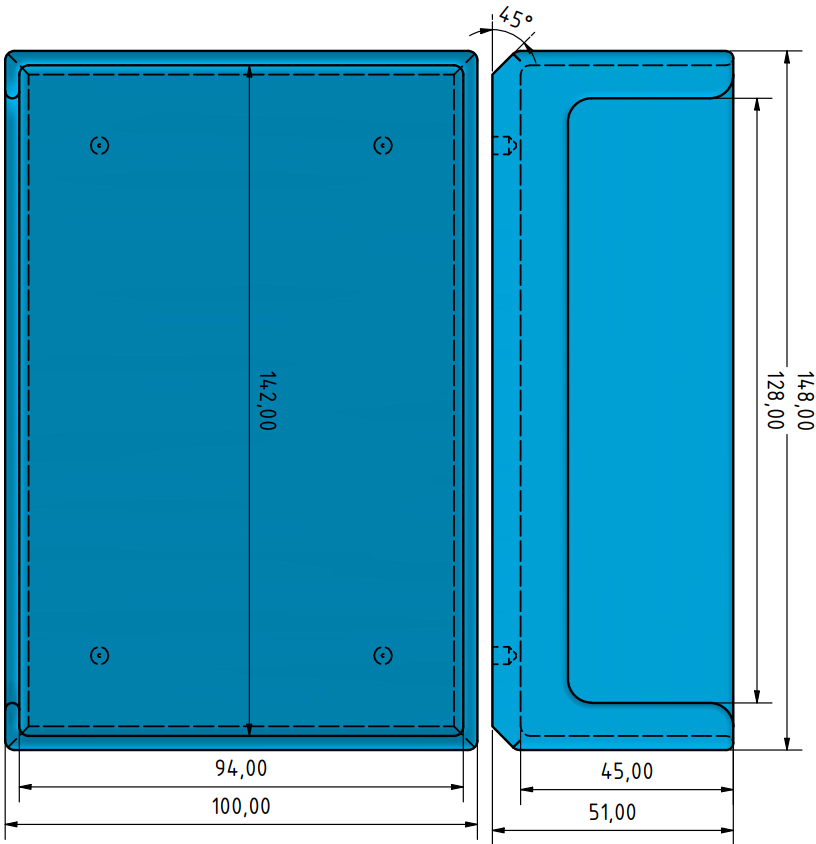
\includegraphics[width=0.8\textwidth]{06disenoConceptual/img/canecas/canecaMedidas.png}
    \caption{Vistas ortogonales de la caneca final con dimensiones principales. Vista superior: 100 mm × 94 mm exteriores, interior de 142 mm de profundidad. Vista lateral: altura total de 148 mm (128 mm útiles), profundidad de 51 mm (45 mm útiles). Se observa el chaflán de 45° para la guía de la tapa deslizante y las posiciones de los insertos roscados M3.}
    \label{fig:canecaMedidas}
\end{figure}

\paragraph{Sistema de Fijación con Insertos Térmicos}

Se implementó un sistema de fijación mediante cuatro insertos roscados M3 para plástico ubicados en la base de la caneca. Estos insertos se instalan mediante inserción térmica: se calientan y se introducen en cavidades cilíndricas diseñadas específicamente, donde el plástico circundante se funde parcialmente y fluye hacia las ranuras del inserto, creando una unión mecánica permanente al enfriarse.

Este sistema ofrece múltiples ventajas:
\begin{itemize}
    \item Los tornillos M3 que fijan la caneca a la plataforma quedan ocultos en la cara inferior, eliminando elementos visuales en la superficie superior
    \item Las roscas metálicas resisten ciclos repetidos de montaje/desmontaje sin degradación
    \item No se requieren tuercas, simplificando el ensamblaje
    \item La superficie superior de la caneca queda completamente limpia, optimizando el desempeño de los algoritmos de visión por computador
\end{itemize}

\paragraph{Separadores de Altura}

Se incorporaron cuatro separadores entre la plataforma base y la caneca. Estos separadores cumplen dos funciones esenciales:

\begin{enumerate}
    \item Nivelar la altura de las canecas con la zona de recolección, que es una pieza elevada respecto a la plataforma base
    \item Proporcionar el espacio necesario para que la tapa deslizante pueda desplazarse completamente y cerrar la caneca
\end{enumerate}

\paragraph{Ensamble Completo}

El subconjunto completo de la zona de depósito se presenta en la Figura \ref{fig:ensambleCanecaTapaSlide}.

\begin{figure}[H]
    \centering
    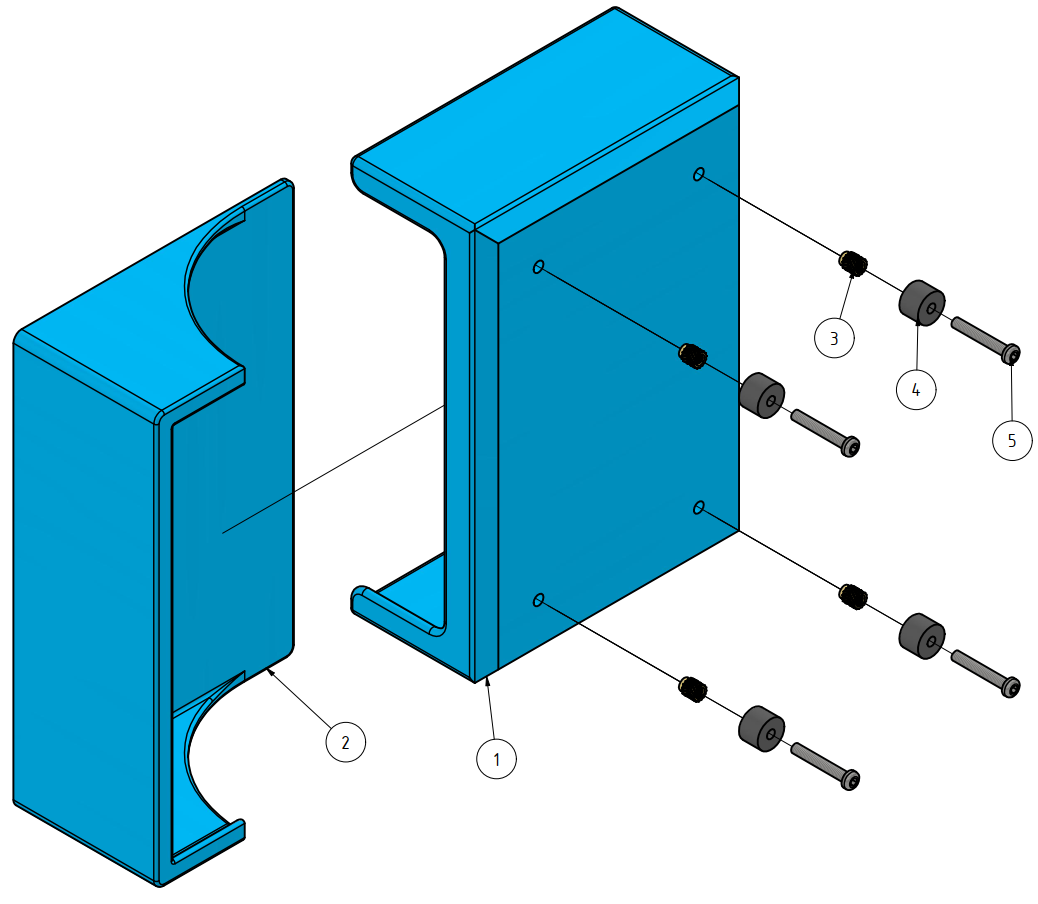
\includegraphics[width=0.8\textwidth]{06disenoConceptual/img/canecas/ensambleCanecaTapaSlide.png}
    \caption{Ensamble explosionado del conjunto de zona de depósito. (1) Cuerpo de la caneca fabricado mediante FDM, (2) Tapa deslizante, (3) Insertos roscados M3 de latón para instalación térmica, (4) Separadores de altura, (5) Tornillos M3 × 20 mm que atraviesan separadores y caneca para fijarse en insertos roscados de la plataforma base.}
    \label{fig:ensambleCanecaTapaSlide}
\end{figure}

\begin{table}[H]
\centering
\caption{Lista de materiales del conjunto de zona de depósito}
\label{tab:bom_caneca}
\small
\begin{tabular}{|c|l|c|l|l|}
\hline
\textbf{\#} & \textbf{Componente} & \textbf{Cant.} & \textbf{Fabricación} & \textbf{Material} \\
\hline
1 & Caneca & 1 & FDM & PLA/ABS \\
2 & Tapa deslizante & 1 & FDM & PLA/ABS \\
3 & Inserto roscado M3 & 4 & Comercial & Latón \\
4 & Separador & 4 & FDM & PLA/ABS \\
5 & Tornillo M3 × 20 mm & 4 & Comercial & Acero \\
\hline
\end{tabular}
\end{table}

El diseño final de las zonas de depósito representa una solución optimizada que equilibra accesibilidad robótica, simplicidad de manufactura, robustez mecánica y compatibilidad con sistemas de visión por computador, resolviendo todas las deficiencias identificadas en la iteración inicial.
\subsection{Diseño de la Zona de Recolección}

La zona de recolección constituye el área donde se posicionan los objetos a clasificar antes de su manipulación por el robot. Su diseño se fundamentó en criterios de accesibilidad robótica, optimización para visión por computador y aprovechamiento del espacio disponible en la plataforma.

\subsubsection{Configuración Geométrica y Ubicación}

El área de recolección se definió a partir del espacio disponible en el layout una vez posicionados la base del manipulador y las cuatro zonas de depósito. Como se observa en el layout de la Figura \ref{fig:layout2}, la zona de recolección ocupa el área circular central delimitada por estos componentes.

La ubicación centrada en la plataforma base ofrece ventajas significativas:

\begin{itemize}
    \item \textbf{Optimización del campo visual}: La posición central respecto a la cámara superior facilita la captura de imágenes con iluminación uniforme y mínima distorsión perspectiva
    \item \textbf{Accesibilidad robótica}: Todos los puntos de la zona de recolección se encuentran dentro del alcance efectivo del manipulador sin requerir configuraciones extremas
    \item \textbf{Simetría operativa}: La distribución equidistante respecto a las cuatro zonas de depósito simplifica la planificación de trayectorias
\end{itemize}

\begin{figure}[H]
    \centering
    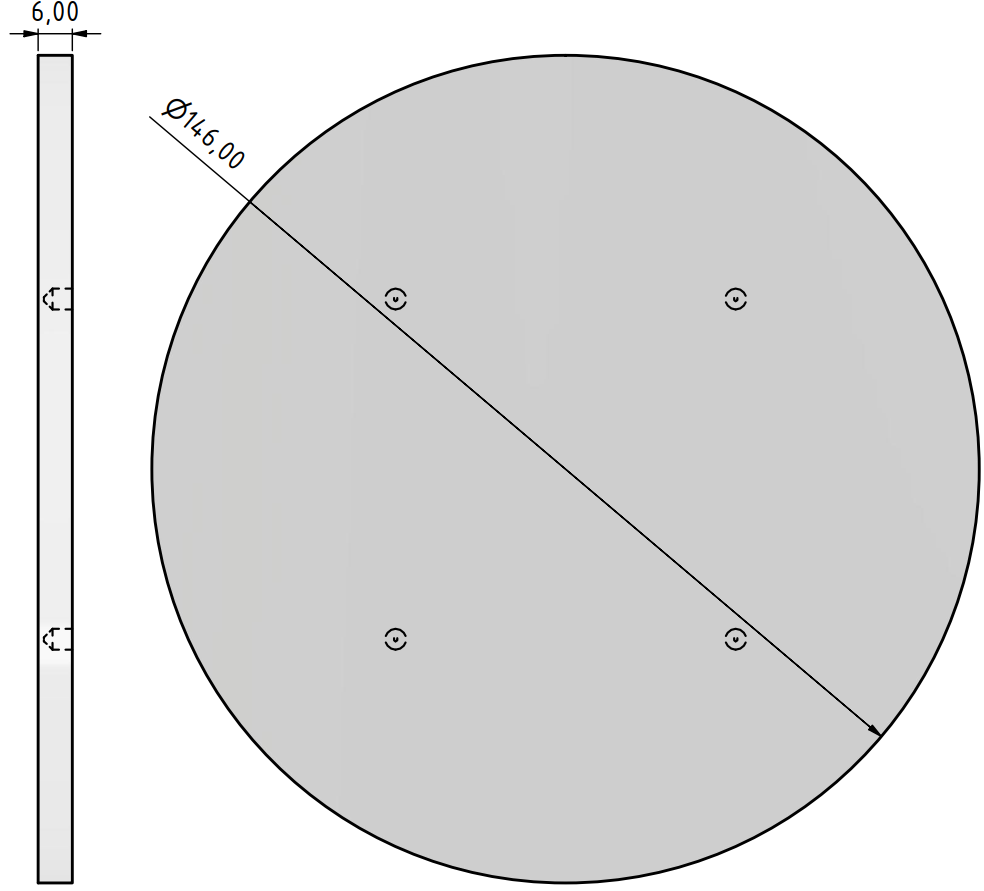
\includegraphics[width=0.6\textwidth]{06disenoConceptual/img/zonaRecoleccion/zonaRecoleccionRedonda.png}
    \caption{Vista superior de la zona de recolección con dimensiones principales. Diámetro exterior: Ø146 mm. Altura: 6 mm mínimo (determinado por el alojamiento de insertos roscados M3 en la cara inferior). Se observan cuatro agujeros ciegos para instalación de insertos roscados distribuidos simétricamente.}
    \label{fig:zonaRecoleccionRedonda}
\end{figure}

\subsubsection{Selección de Color y Acabado Superficial}

Se seleccionó el color blanco para la superficie de la zona de recolección por razones relacionadas con el desempeño de los algoritmos de visión por computador:

\begin{enumerate}
    \item \textbf{Máximo contraste con objetos}: La superficie blanca proporciona contraste elevado con objetos de colores típicamente utilizados en tareas de clasificación (rojo, verde, azul, amarillo, negro)
    
    \item \textbf{Balance de blancos}: Facilita la calibración automática del balance de blancos de la cámara, mejorando la reproducción cromática de los objetos
    
    \item \textbf{Iluminación difusa}: La superficie blanca refleja luz de manera más uniforme que colores oscuros, reduciendo sombras pronunciadas que puedan interferir con la segmentación de objetos
    
    \item \textbf{Contraste con plataforma base}: La zona blanca sobre la plataforma base negra crea una delimitación visual clara del área de trabajo
\end{enumerate}

\subsubsection{Sistema de Fijación}

La zona de recolección se fija a la plataforma base mediante cuatro insertos roscados M3 para plástico instalados en la cara inferior. Este sistema proporciona múltiples ventajas:

\begin{itemize}
    \item \textbf{Superficie superior limpia}: Al ubicarse los insertos y tornillos en la cara inferior, la superficie superior queda completamente libre de elementos de fijación visibles, eliminando potenciales interferencias con los algoritmos de visión
    
    \item \textbf{Simplificación visual}: La zona de recolección se presenta como una superficie circular blanca uniforme, facilitando su identificación automática y la detección de objetos sobre ella
    
    \item \textbf{Restricción de altura mínima}: Los insertos roscados M3 requieren una profundidad de alojamiento que establece una altura mínima de 6 mm para la zona de recolección, valor que resulta adecuado para proporcionar un pequeño escalón que delimita visualmente el área
\end{itemize}

\subsubsection{Ensamble del Conjunto}

El conjunto completo de la zona de recolección se presenta en la Figura \ref{fig:ensambleZonaRecoleccion}.

\begin{figure}[H]
    \centering
    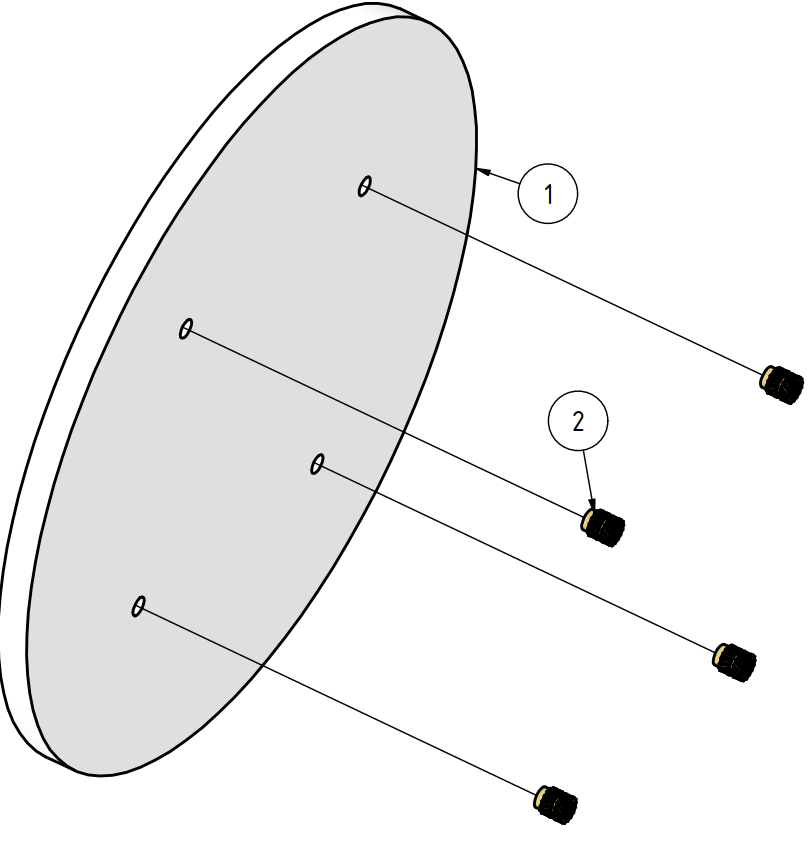
\includegraphics[width=0.55\textwidth]{06disenoConceptual/img/zonaRecoleccion/ensambleZonaRecoleccion.png}
    \caption{Ensamble explosionado de la zona de recolección. (1) Disco circular fabricado mediante FDM en filamento blanco (PLA o ABS), (2) Tornillos M3 × 15 mm que atraviesan la plataforma base y se enroscan en los insertos roscados ubicados en la cara inferior del disco.}
    \label{fig:ensambleZonaRecoleccion}
\end{figure}

\begin{table}[H]
\centering
\caption{Lista de materiales de la zona de recolección}
\label{tab:bom_zona_recoleccion}
\small
\begin{tabular}{|c|l|c|l|l|}
\hline
\textbf{\#} & \textbf{Componente} & \textbf{Cant.} & \textbf{Fabricación} & \textbf{Material} \\
\hline
1 & Zona de recolección & 1 & FDM & PLA/ABS blanco \\
2 & Inserto roscado M3 & 4 & Comercial & Latón \\
3 & Tornillo M3 × 15 mm & 4 & Comercial & Acero \\
\hline
\end{tabular}
\end{table}

La simplicidad de este diseño contrasta favorablemente con la complejidad de las canecas de la primera iteración, demostrando que la funcionalidad óptima no siempre requiere soluciones elaboradas. La zona de recolección cumple eficientemente su propósito mediante una geometría simple, un sistema de fijación robusto y una selección de color fundamentada en principios de visión por computador.
\subsection{Diseño de la Base del Manipulador}

La base del manipulador constituye la interfaz mecánica entre el robot PhantomX Pincher y la plataforma del kit. Su diseño se fundamentó en la preservación de características funcionales de la base original, incorporando mejoras estructurales y adaptaciones específicas para el nuevo sistema.

\subsubsection{Análisis de la Base Original}

La base original del robot PhantomX Pincher AX-12 (Figura \ref{fig:ensambleOldBaseArm}) sirvió como referencia para el diseño, proporcionando información valiosa sobre dimensiones, sistemas de fijación y requisitos operativos.

\begin{figure}[H]
    \centering
    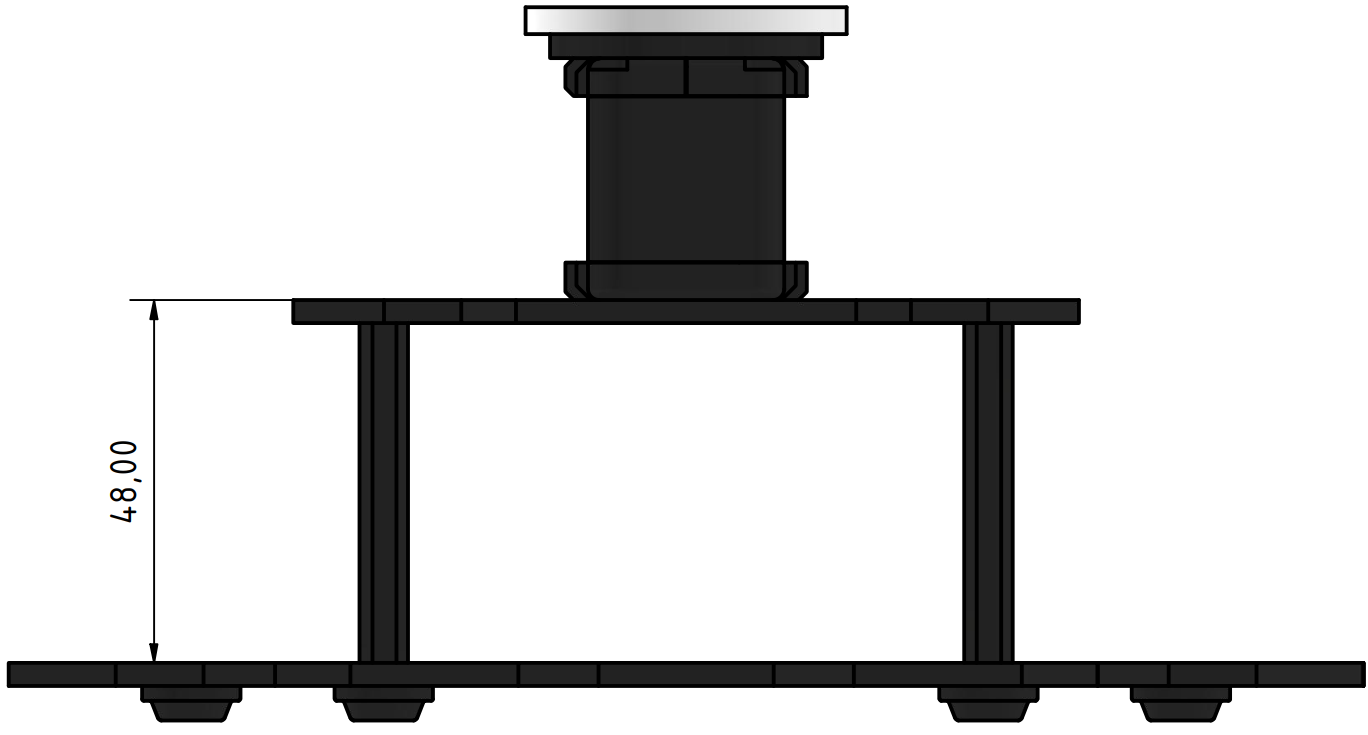
\includegraphics[width=0.6\textwidth]{06disenoConceptual/img/oldArm/medidaBaseArmOld.png}
    \caption{Base original del robot PhantomX Pincher AX-12. (1) Base superior de acrílico que soporta el servomotor principal, (2) Base inferior de acrílico para fijación a superficies, (3) Cuatro espaciadores hexagonales de nylon M3, (4) Manipulador PhantomX Pincher. Se observan las ranuras laterales para paso de cableado.}
    \label{fig:ensambleOldBaseArm}
\end{figure}

\begin{table}[H]
\centering
\caption{Componentes de la base original del PhantomX Pincher AX-12}
\label{tab:base_original}
\small
\begin{tabular}{|c|l|c|l|}
\hline
\textbf{\#} & \textbf{Componente} & \textbf{Cant.} & \textbf{Material} \\
\hline
1 & Base superior de manipulador & 1 & Acrílico \\
2 & Base inferior de manipulador & 1 & Acrílico \\
3 & Espaciador hexagonal de nylon M3 & 4 & Nylon \\
4 & Manipulador & 1 & --- \\
\hline
\end{tabular}
\end{table}

La altura de la base original es de 48 mm (Figura \ref{fig:medidaBaseArmOld}), dimensión que se conservó en el diseño final para mantener la compatibilidad cinemática con los algoritmos de control existentes.

\begin{figure}[H]
    \centering
    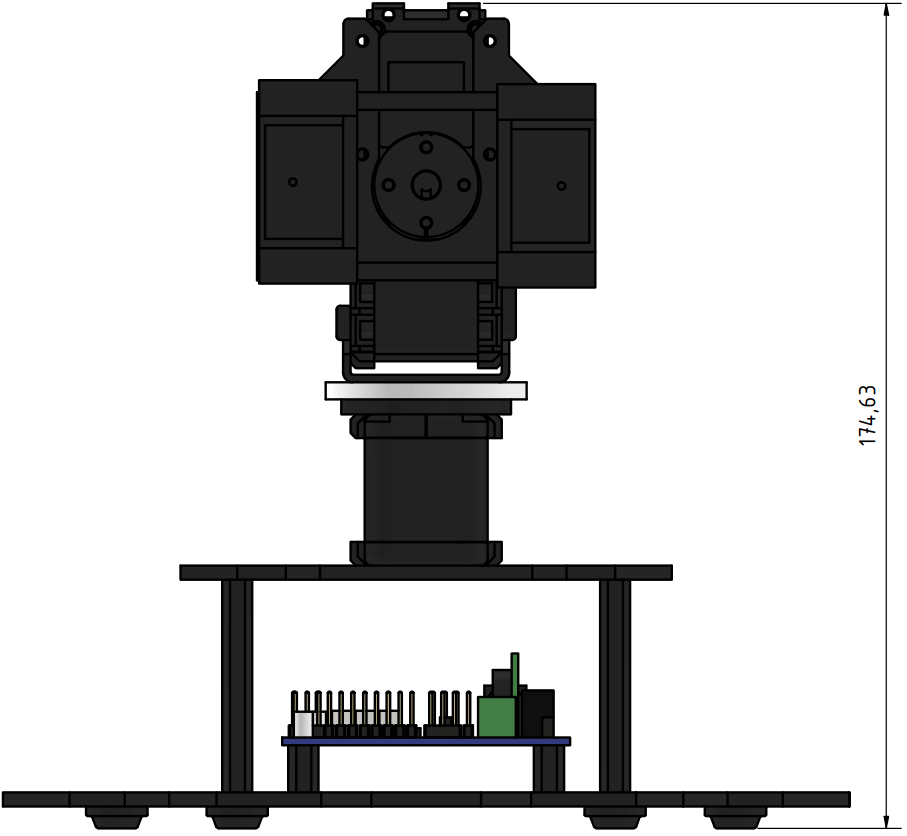
\includegraphics[width=0.5\textwidth]{06disenoConceptual/img/oldArm/medidasPXPAX-12old.png}
    \caption{Vista lateral de la base original mostrando la altura total de 48 mm desde la superficie de montaje hasta la interfaz del manipulador.}
    \label{fig:medidaBaseArmOld}
\end{figure}

\subsubsection{Características Preservadas del Diseño Original}

Del diseño original se conservaron los siguientes elementos funcionales:

\begin{itemize}
    \item \textbf{Sistema de espaciadores hexagonales}: Se mantiene el uso de cuatro espaciadores M3 para fijación del manipulador, garantizando compatibilidad mecánica
    \item \textbf{Ranuras laterales de cableado}: Se preservan las dos aberturas laterales que permiten el paso de cables desde la zona de electrónica hasta el manipulador
    \item \textbf{Altura estándar}: Se conserva la altura de 48 mm para mantener la compatibilidad con la cinemática del robot
\end{itemize}

\subsubsection{Modificaciones e Innovaciones del Diseño}

El diseño final incorpora mejoras significativas respecto a la base original:

\paragraph{Eliminación de la Base Inferior}

Se suprimió la placa inferior de la base original, ya que la plataforma del kit cumple esta función. Esta simplificación reduce:
\begin{itemize}
    \item Número de componentes del sistema
    \item Costo de fabricación
    \item Peso total del conjunto
    \item Complejidad de ensamblaje
\end{itemize}

\paragraph{Integración con Sistema de Vacío}

Se diseñó una cavidad semicircular en la parte posterior de la base (visible en la Figura \ref{fig:medidasBaseArm}) para alojar la bomba de vacío. Esta integración permite:
\begin{itemize}
    \item Aprovechamiento óptimo del espacio disponible
    \item Proximidad entre bomba de vacío y manipulador, minimizando longitud de mangueras
    \item Protección parcial de la bomba dentro del volumen de la base
\end{itemize}

\begin{figure}[H]
    \centering
    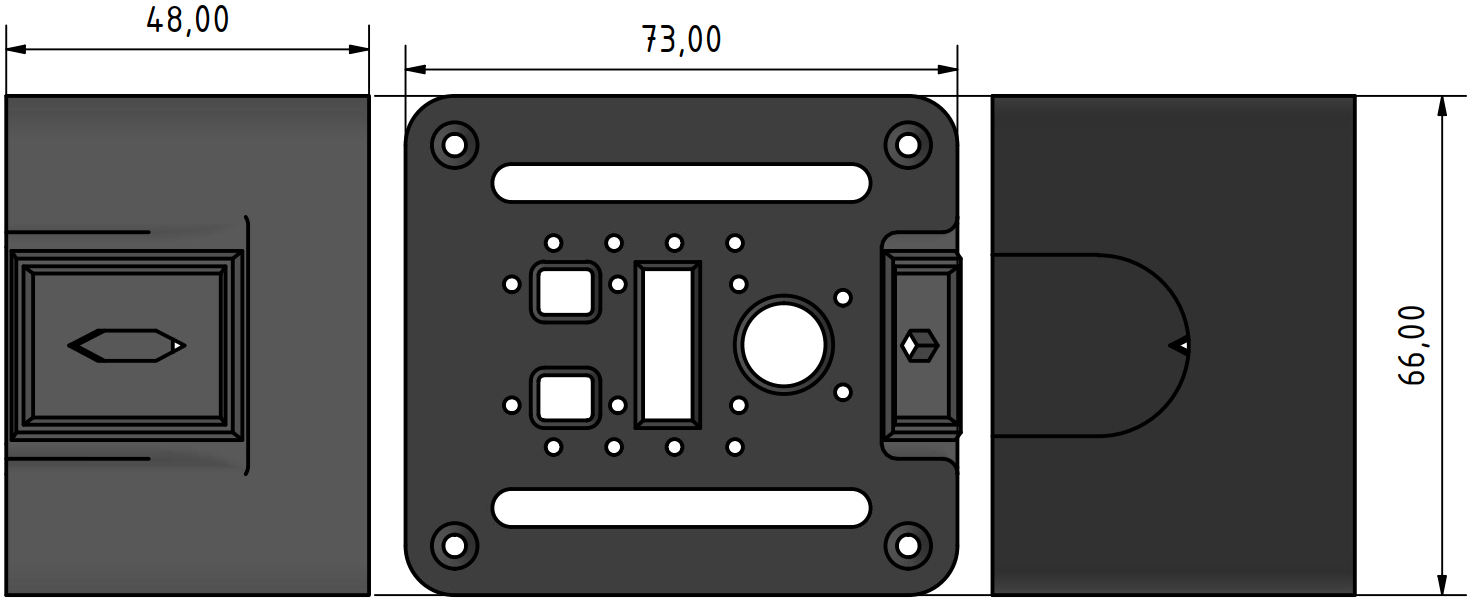
\includegraphics[width=0.75\textwidth]{06disenoConceptual/img/baseArm/medidasBaseArm.png}
    \caption{Vista superior de la base del manipulador con dimensiones principales. Dimensiones exteriores: 73 mm × 66 mm. Se observan: cavidad semicircular posterior de 48 mm de diámetro para alojamiento de bomba de vacío, ranuras laterales de cableado, patrón de montaje para espaciadores hexagonales M3, y diversas perforaciones para paso de cables y ventilación.}
    \label{fig:medidasBaseArm}
\end{figure}

\paragraph{Sistema de Identificación}

Dado que se fabricarán siete kits completos, se incorporó un sistema de identificación mediante una placa plástica intercambiable montada en el frente de la base. Esta ubicación frontal fue seleccionada por:
\begin{itemize}
    \item Alta visibilidad desde cualquier ángulo de aproximación al kit
    \item Facilidad de lectura para usuarios y personal de laboratorio
    \item Posibilidad de reemplazo sin desmontar el manipulador
\end{itemize}

\paragraph{Mejora del Material de Espaciadores}

Se sustituyeron los espaciadores hexagonales de nylon por espaciadores de latón M3 × 30 mm. Esta modificación se fundamentó en la experiencia operativa: durante el desmontaje del manipulador de su base original, varios espaciadores de nylon se fracturaron. El latón ofrece:
\begin{itemize}
    \item Mayor resistencia mecánica a cargas de tracción y compresión
    \item Durabilidad superior frente a ciclos repetidos de montaje/desmontaje
    \item Roscas más resistentes al desgaste
    \item Mejor tolerancia dimensional
\end{itemize}

\paragraph{Soporte Estructural Mejorado}

A diferencia de la base original que se apoyaba únicamente en cuatro puntos (los espaciadores), el diseño final apoya todo su perímetro sobre la plataforma base. Esta configuración proporciona:
\begin{itemize}
    \item Mayor rigidez estructural del conjunto
    \item Distribución más uniforme de cargas operativas
    \item Reducción de vibraciones durante movimientos del manipulador
    \item Estabilidad mejorada para operaciones de alta precisión
\end{itemize}

\subsubsection{Restricciones Dimensionales}

Las dimensiones en planta de la base (73 mm × 66 mm) se determinaron considerando las restricciones espaciales impuestas por el layout de la plataforma (Figura \ref{fig:layout2}). Específicamente, el área ocupada por la base no debe interferir con el cierre de las tapas deslizantes de las canecas adyacentes. Un incremento dimensional de la base invadiría la trayectoria de las tapas, impidiendo el cierre completo de las zonas de depósito.

\subsubsection{Ensamble del Conjunto}

El conjunto completo de la base del manipulador se presenta en la Figura \ref{fig:ensambleBaseArm}.

\begin{figure}[H]
    \centering
    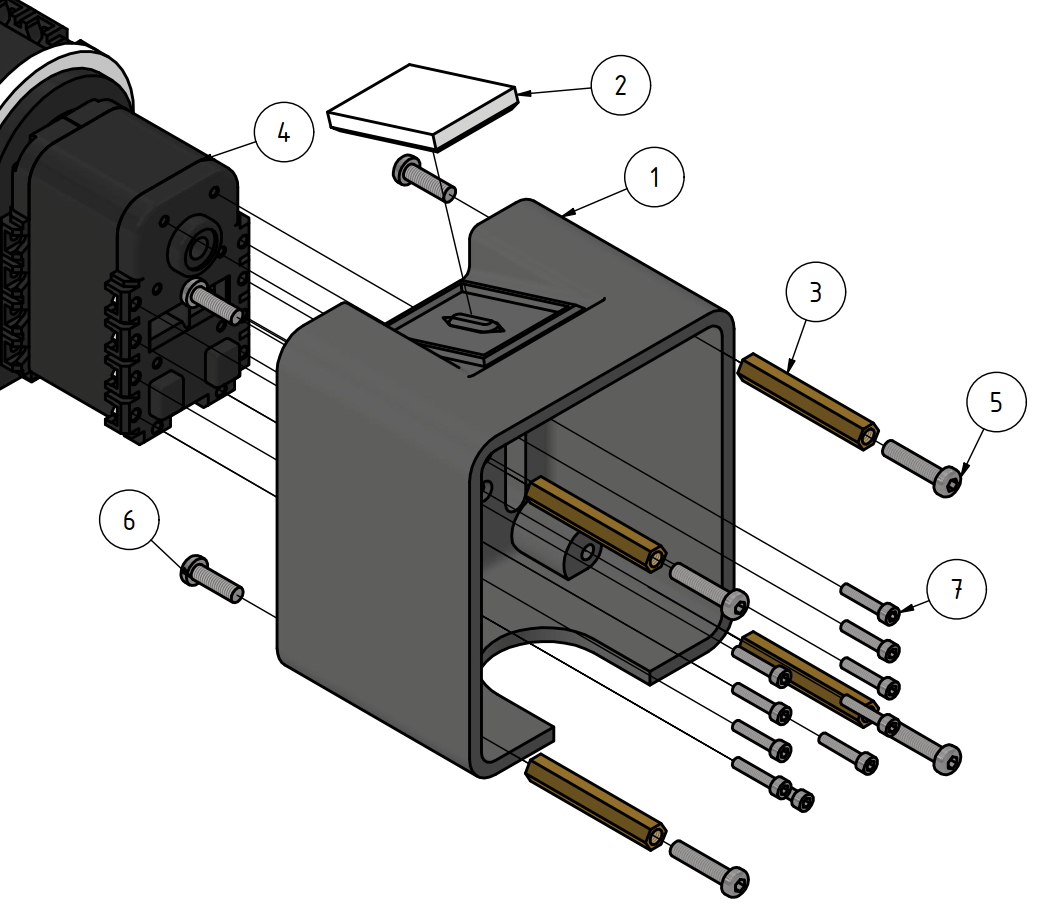
\includegraphics[width=0.85\textwidth]{06disenoConceptual/img/baseArm/ensambleBaseArm.png}
    \caption{Ensamble explosionado de la base del manipulador. (1) Cuerpo de la base fabricado mediante FDM, (2) Placa de identificación numérica intercambiable, (3) Cuatro espaciadores hexagonales de latón M3 × 30 mm, (4) Manipulador PhantomX Pincher, (5) Tornillos M3 × 14 mm para fijación de espaciadores a la base, (6) Tornillos M3 × 10 mm para fijación de la placa identificadora, (7) Tornillos M2 × 10 mm (10 unidades) para fijación del manipulador a los espaciadores.}
    \label{fig:ensambleBaseArm}
\end{figure}

\begin{table}[H]
\centering
\caption{Lista de materiales de la base del manipulador}
\label{tab:bom_base_manipulador}
\small
\begin{tabular}{|c|l|c|l|l|}
\hline
\textbf{\#} & \textbf{Componente} & \textbf{Cant.} & \textbf{Fabricación} & \textbf{Material} \\
\hline
1 & Base de manipulador & 1 & FDM & ABS/PLA \\
2 & Placa de número identificador & 1 & FDM & ABS/PLA \\
3 & Espaciador hexagonal M3 × 30 mm & 4 & Comercial & Latón \\
4 & Manipulador & 1 & --- & --- \\
5 & Tornillo M3 × 14 mm & 4 & Comercial & Acero \\
6 & Tornillo M3 × 10 mm & 4 & Comercial & Acero \\
7 & Tornillo M2 × 10 mm & 10 & Comercial & Acero \\
\hline
\end{tabular}
\end{table}

Los espaciadores hexagonales se fijan a la base mediante tornillos M3 × 14 mm que se enroscan directamente en el latón. El manipulador se monta sobre estos espaciadores utilizando los tornillos M2 × 10 mm originales del robot, reutilizando componentes existentes y reduciendo costos.

El diseño final de la base del manipulador representa una evolución optimizada del concepto original, integrando mejoras estructurales, consideraciones de manufactura, y requisitos específicos del sistema completo del kit educativo.
\subsection{Diseño del Sistema de Succión con Ventosa}

El sistema de efector final del kit incorpora un mecanismo de succión por vacío como alternativa al gripper mecánico original del PhantomX Pincher. Este sistema permite la manipulación de objetos ligeros mediante adhesión neumática, ampliando las capacidades didácticas del kit.

\subsubsection{Condiciones de Diseño}

Las restricciones y requerimientos técnicos del sistema de succión son:

\begin{itemize}
    \item Voltaje de alimentación disponible: 12 V DC (fuente del robot)
    \item Área típica de objetos a manipular: 25 mm × 25 mm
    \item Diámetro de ventosa seleccionada: 15 mm
    \item Restricción espacial: La bomba debe caber dentro de la base del manipulador
    \item Compatibilidad neumática: Conexión a mangueras de 6 mm de diámetro
\end{itemize}

\subsubsection{Evaluación de Bombas de Vacío}

Se evaluaron dos bombas de vacío miniatura compatibles con la alimentación de 12 V del robot:

\paragraph{Bomba Mini Air Pump 370A}

Microbomba de vacío diseñada específicamente para succión de aire. Utiliza motor tipo 370 con diafragma, genera vacío máximo de -65 kPa. Dimensiones compactas: aproximadamente 27 mm de diámetro × 58 mm de largo, peso 60 g. La boca de salida permite conexión directa a mangueras neumáticas de 6 mm sin acoples adicionales.

\paragraph{Bomba R385 Diaphragm Pump}

Bomba de diafragma diseñada para bombeo de agua, adaptable para aire. Opera entre 6 y 12 V DC con consumo de 0.5-1 A. Capacidad de succión máxima: 2 m de columna de agua (equivalente a aproximadamente 19.6 kPa). Dimensiones: 90 mm × 40 mm × 35 mm, peso 112 g. Diámetro de boca: 7-8.5 mm externo, requiere acople para mangueras de 6 mm.

\subsubsection{Comparación Técnica}

La Tabla \ref{tab:comparacion_bombas} resume las especificaciones técnicas de ambas bombas.

\begin{table}[H]
\centering
\caption{Comparación de especificaciones técnicas de bombas de vacío}
\label{tab:comparacion_bombas}
\small
\begin{tabular}{|l|c|c|}
\hline
\textbf{Parámetro} & \textbf{Bomba 370A} & \textbf{Bomba R385} \\
\hline
Voltaje nominal & DC 12 V & DC 6-12 V \\
Corriente & 280-420 mA & 500-700 mA \\
Potencia aproximada & 3.4-5 W & 4.8-6 W \\
Tipo de bomba & Vacío (aire) & Diafragma (agua/aire) \\
Vacío máximo & -65 kPa & -19.6 kPa (2 m col. agua) \\
Flujo de aire & 3.5-4.5 LPM & 1.5-2 L/min \\
Dimensiones & Ø27 × 58 mm & 90 × 40 × 35 mm \\
Peso & 60 g & 112 g \\
Ruido & 55-60 dB & $<$30 dB (agua) \\
Diámetro de boca & 4.2-6 mm & Int. 6 mm, ext. 8.5 mm \\
Conexión neumática & Directa Ø6 mm & Requiere acople \\
Vida útil & $>$50,000 ciclos & 2,500 h \\
\hline
\end{tabular}
\end{table}

\subsubsection{Análisis de Capacidad de Levantamiento}

Para determinar la capacidad de cada bomba, se calculó la fuerza de succión generada sobre el área efectiva de la ventosa.

\paragraph{Datos del Sistema}

\begin{itemize}
    \item Diámetro de ventosa: $d = 15$ mm $= 0.015$ m
    \item Radio de ventosa: $r = 7.5$ mm $= 0.0075$ m
    \item Área efectiva: $A = \pi r^{2} = \pi \times (0.0075)^{2} = 1.7671 \times 10^{-4}$ m$^{2}$
    \item Aceleración gravitacional: $g = 9.81$ m/s$^{2}$
\end{itemize}

\paragraph{Modelo Teórico}

La fuerza de succión se calcula mediante:

\begin{equation}
F = \Delta P \times A
\end{equation}

donde $F$ es la fuerza de succión [N], $\Delta P$ es la presión de vacío generada [Pa], y $A$ es el área efectiva de la ventosa [m$^{2}$].

La masa máxima levantable se obtiene de:

\begin{equation}
m = \frac{F}{g}
\end{equation}

\paragraph{Cálculo para Bomba 370A}

Vacío máximo: -65 kPa = 65,000 Pa

\begin{align}
F_{370} &= 65{,}000 \times 1.7671 \times 10^{-4} = 11.49 \text{ N} \\
m_{370} &= \frac{11.49}{9.81} = 1.17 \text{ kg}
\end{align}

\paragraph{Cálculo para Bomba R385}

Capacidad de succión: 2 m de columna de agua

Conversión a presión:
\begin{equation}
\Delta P = \rho \cdot g \cdot h = 1{,}000 \times 9.81 \times 2 = 19{,}620 \text{ Pa} \approx 19.6 \text{ kPa}
\end{equation}

\begin{align}
F_{R385} &= 19{,}620 \times 1.7671 \times 10^{-4} = 3.47 \text{ N} \\
m_{R385} &= \frac{3.47}{9.81} = 0.354 \text{ kg} = 354 \text{ g}
\end{align}

\paragraph{Resumen de Resultados}

La Tabla \ref{tab:capacidad_levantamiento} resume la capacidad de levantamiento de ambas bombas.

\begin{table}[H]
\centering
\caption{Capacidad de levantamiento de bombas de vacío}
\label{tab:capacidad_levantamiento}
\small
\begin{tabular}{|l|c|c|}
\hline
\textbf{Parámetro} & \textbf{Bomba 370A} & \textbf{Bomba R385} \\
\hline
Vacío máximo (kPa) & -65 & -19.6 \\
Fuerza de succión (N) & 11.49 & 3.47 \\
Masa máxima teórica (kg) & 1.17 & 0.354 \\
Factor de seguridad ×0.5 & 0.585 kg & 0.177 kg \\
\hline
\end{tabular}
\end{table}

\paragraph{Consideraciones Prácticas}

Los valores calculados son teóricos y asumen sellado perfecto entre ventosa y objeto. En la práctica, la fuerza efectiva se reduce por:

\begin{itemize}
    \item Fugas de aire entre ventosa y superficie
    \item Rugosidad superficial del objeto
    \item Pérdidas en mangueras y conexiones neumáticas
    \item Deformación de la ventosa
    \item Tiempo de establecimiento del vacío
\end{itemize}

Se recomienda aplicar un factor de seguridad de 2 (utilizar 50\% de capacidad teórica). Con este factor, la bomba 370A puede levantar de manera confiable objetos de hasta 585 g, mientras que la R385 está limitada a aproximadamente 177 g.

\subsubsection{Justificación de la Selección}

La bomba 370A fue seleccionada por las siguientes razones:

\begin{enumerate}
    \item \textbf{Capacidad de vacío superior}: Genera -65 kPa, más de tres veces mayor que los -19.6 kPa de la R385, resultando en fuerza de succión de 11.49 N frente a 3.47 N
    
    \item \textbf{Diseño compacto}: Dimensiones de Ø27 × 58 mm y peso de 60 g, significativamente más pequeña que la R385 (90 × 40 × 35 mm, 112 g), facilitando integración en la base del robot
    
    \item \textbf{Conexión directa}: Boca compatible con mangueras de 6 mm sin acoples adicionales. La R385 requiere acople intermedio
    
    \item \textbf{Menor consumo energético}: Consume 280-420 mA frente a 500-1,000 mA de la R385, reduciendo carga sobre la fuente de alimentación
    
    \item \textbf{Diseño específico para vacío}: Optimizada para succión de aire, a diferencia de la R385 diseñada para bombeo de agua
    
    \item \textbf{Costo}: Precio más accesible, compatible con el presupuesto del proyecto
\end{enumerate}

\subsubsection{Selección de Ventosa}

La selección de la ventosa se fundamentó en dos criterios principales: disponibilidad comercial en el mercado nacional e internacional, y compatibilidad dimensional con los objetos a manipular.

\paragraph{Criterios de Dimensionamiento}

Los objetos de clasificación contemplados para el kit poseen dimensiones estándar de 25 mm × 25 mm. Para garantizar un margen de seguridad adecuado que permita variaciones en el posicionamiento del manipulador y tolerancias en la ubicación de los objetos, se estableció que la ventosa debía proporcionar una holgura mínima de 5 mm respecto a los bordes del objeto.

Con base en este criterio, se seleccionó una ventosa de 15 mm de diámetro, que proporciona:

\begin{itemize}
    \item Holgura lateral: $\frac{25 - 15}{2} = 5$ mm por cada lado
    \item Área de contacto suficiente para garantizar adhesión confiable
    \item Compatibilidad con objetos de dimensiones variables entre 15 mm y 30 mm aproximadamente
\end{itemize}

Esta configuración permite que, incluso con desalineamientos moderados del manipulador (±5 mm), la ventosa pueda establecer contacto efectivo con la superficie del objeto y generar el vacío necesario para su levantamiento.

\paragraph{Ventosa Seleccionada}

Se seleccionó la ventosa modelo PAK-15, disponible comercialmente a través de proveedores internacionales. Esta ventosa presenta las siguientes características:

\begin{itemize}
    \item Diámetro: 15 mm
    \item Material: Silicona o caucho nitrílico (NBR), resistente a deformación y degradación
    \item Conexión: Compatible con mangueras neumáticas de 4-6 mm de diámetro interno
    \item Tipo: Ventosa plana de propósito general, adecuada para superficies lisas o ligeramente texturizadas
    \item Costo: Accesible, compatible con el presupuesto del proyecto
\end{itemize}

La ventosa PAK-15 es ampliamente utilizada en sistemas de automatización ligera y pick-and-place debido a su versatilidad, durabilidad y facilidad de instalación. Su diseño permite un sellado efectivo sobre superficies planas, maximizando la transmisión del vacío generado por la bomba 370A hacia el objeto a manipular.

\paragraph{Consideraciones de Integración}

La ventosa se conecta a la bomba de vacío mediante una manguera neumática de 6 mm de diámetro exterior (4 mm de diámetro interior). Esta configuración minimiza las pérdidas de vacío y garantiza tiempos de respuesta rápidos durante las operaciones de succión y liberación de objetos.

El montaje de la ventosa en el efector final del manipulador se realiza mediante un soporte diseñado específicamente que permite:

\begin{itemize}
    \item Alineación precisa con el eje vertical del manipulador
    \item Conexión segura de la manguera neumática sin restricciones de movimiento
    \item Acceso visual de la cámara superior a los objetos durante la aproximación
    \item Reemplazo rápido de la ventosa en caso de desgaste o daño
\end{itemize}

\subsubsection{Sistema Completo de Succión por Vacío}

El sistema de succión por vacío integra múltiples subconjuntos y componentes neumáticos que trabajan coordinadamente para permitir la manipulación de objetos mediante adhesión. La Figura \ref{fig:ensambleSuccion} presenta una vista general del sistema completo instalado en el kit.

\begin{figure}[H]
    \centering
    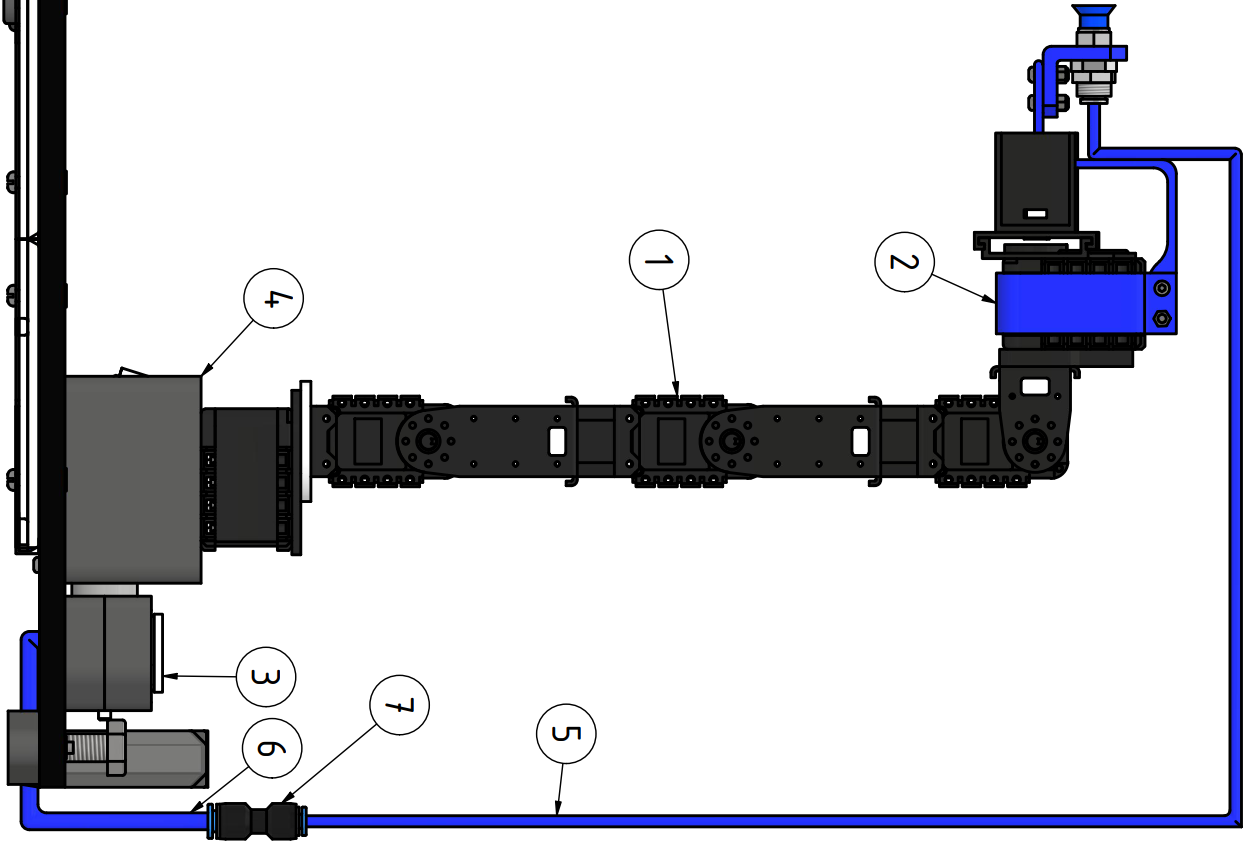
\includegraphics[width=0.95\textwidth]{06disenoConceptual/img/succion/ensambleSuccion.png}
    \caption{Sistema completo de succión por vacío integrado en el kit. (1) Brazo robótico PhantomX Pincher AX-12, (2) Subconjunto de gripper de succión montado en el efector final, (3) Subconjunto de base de bomba de vacío, (4) Subconjunto de base del manipulador, (5) Manguera neumática M4 × 1 m conectando bomba y gripper, (6) Manguera neumática M6 × 30 cm (conexión auxiliar), (7) Acople reductor de 6 mm a 4 mm para compatibilidad entre mangueras y ventosa.}
    \label{fig:ensambleSuccion}
\end{figure}

\begin{table}[H]
\centering
\caption{Componentes principales del sistema de succión}
\label{tab:sistema_succion}
\small
\begin{tabular}{|c|l|c|}
\hline
\textbf{\#} & \textbf{Componente} & \textbf{Cant.} \\
\hline
1 & Brazo robótico PhantomX Pincher AX-12 & 1 \\
2 & Subconjunto de gripper de succión & 1 \\
3 & Subconjunto de base de bomba de vacío & 1 \\
4 & Subconjunto de base de manipulador & 1 \\
5 & Manguera neumática M4 × 1 m & 1 \\
6 & Manguera neumática M6 × 30 cm & 1 \\
7 & Acople reductor 6 mm a 4 mm & 1 \\
\hline
\end{tabular}
\end{table}

El sistema está compuesto principalmente por el subconjunto del gripper de succión (que incluye la ventosa y su soporte), el subconjunto de la bomba de vacío (que aloja la bomba 370A), las mangueras neumáticas que conectan ambos elementos, y el acople reductor que garantiza compatibilidad entre diferentes diámetros. Los demás elementos listados (base del manipulador y brazo robótico) se incluyen en la descripción por su función de soporte estructural y anclaje de los componentes neumáticos.

\subsubsection{Diseño del Subconjunto de Gripper de Succión}

El subconjunto del gripper de succión constituye el efector final del sistema de vacío. Su diseño permite la coexistencia del gripper mecánico original con el sistema de succión, facilitando el cambio rápido entre ambos modos de operación sin necesidad de desmontar completamente ninguno de los dos sistemas.

\begin{figure}[H]
    \centering
    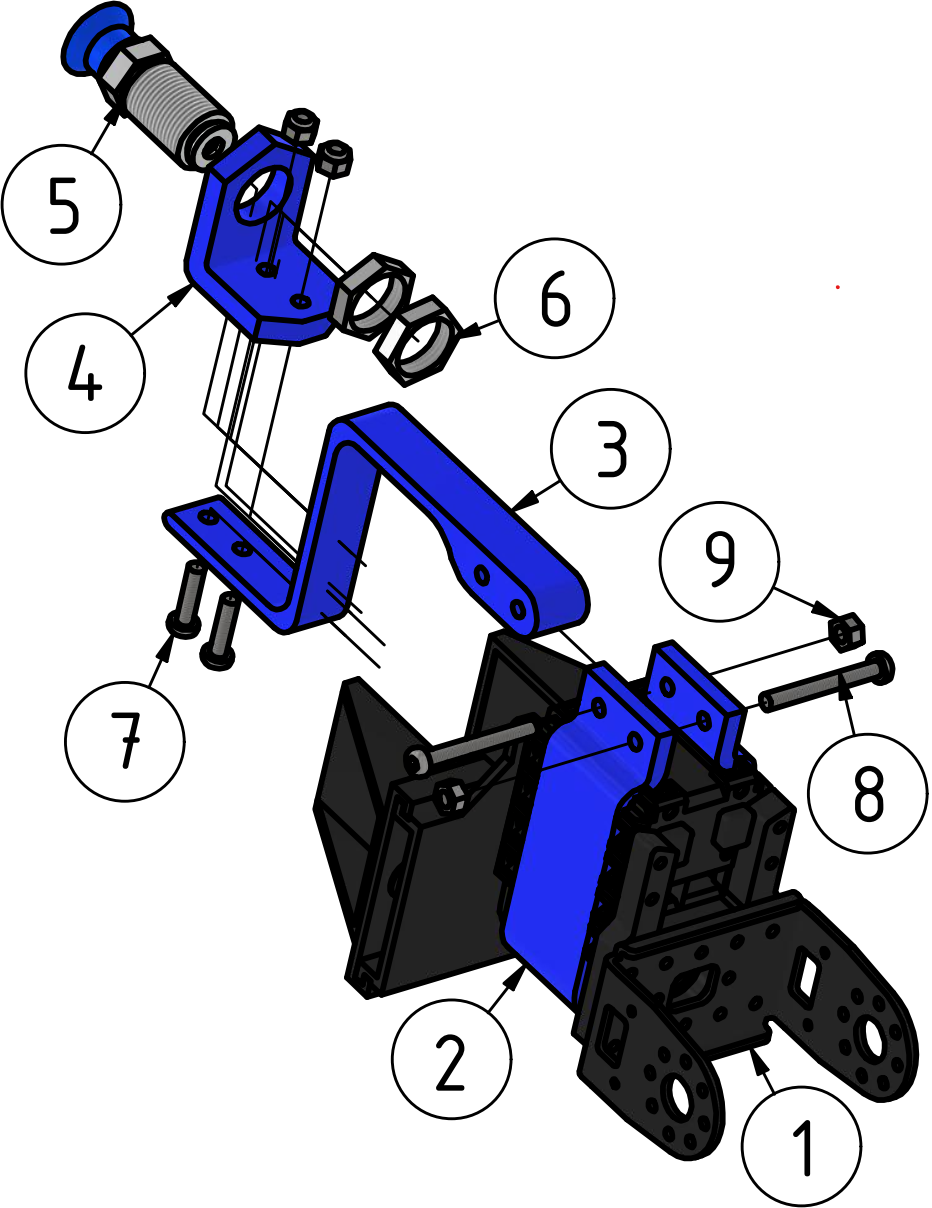
\includegraphics[width=0.65\textwidth]{06disenoConceptual/img/succion/ensambleVentosa.png}
    \caption{Ensamble explosionado del subconjunto de gripper de succión. (1) Gripper de pinza original del robot, (2) Pieza de anclaje al motor del gripper fabricada mediante FDM, (3) Pieza de extensión de ventosa que proporciona separación vertical, (4) Pieza de anclaje de ventosa con conexión neumática, (5) Ventosa PAK-15 de 15 mm de diámetro, (6) Tuercas M12 × 4 mm con paso de rosca 1 mm, (7) Tornillos M3 × 12 mm, (8) Tornillos M3 × 25 mm, (9) Tuercas de seguridad M3 (4 unidades).}
    \label{fig:ensambleVentosa}
\end{figure}

\begin{table}[H]
\centering
\caption{Lista de materiales del subconjunto de gripper de succión}
\label{tab:bom_gripper_succion}
\small
\begin{tabular}{|c|l|c|l|l|}
\hline
\textbf{\#} & \textbf{Componente} & \textbf{Cant.} & \textbf{Fabricación} & \textbf{Material} \\
\hline
1 & Gripper de pinza & 1 & --- & --- \\
2 & Pieza de anclaje a gripper & 1 & FDM & PLA/ABS \\
3 & Pieza de extensión de ventosa & 1 & FDM & PLA/ABS \\
4 & Pieza de anclaje de ventosa & 1 & FDM & PLA/ABS \\
5 & Ventosa PAK-15 & 1 & Comercial & Silicona/NBR \\
6 & Tuerca M12 × 4 mm (paso 1 mm) & 2 & Comercial & Acero \\
7 & Tornillo M3 × 12 mm & 2 & Comercial & Acero \\
8 & Tornillo M3 × 25 mm & 2 & Comercial & Acero \\
9 & Tuerca M3 de seguridad & 4 & Comercial & Acero \\
\hline
\end{tabular}
\end{table}

\paragraph{Estrategia de Diseño Modular}

El diseño del gripper de succión se fundamentó en el principio de modularidad, permitiendo la conversión rápida entre modo de pinza mecánica y modo de succión sin requerir desmontaje extensivo. La pieza de anclaje al gripper se fabrica mediante FDM y se monta directamente sobre el servomotor del gripper original, permaneciendo fija mediante ajuste por fricción sin necesidad de tornillería adicional.

El resto del sistema de succión (extensión, anclaje de ventosa y ventosa) se atornilla a esta pieza base mediante dos tornillos M3. Esta configuración permite:

\begin{itemize}
    \item Cambio entre pinza mecánica y ventosa mediante remoción/instalación de solo dos tornillos
    \item Preservación del gripper original sin modificaciones permanentes
    \item Tiempo de cambio de configuración inferior a 2 minutos
    \item Posibilidad de almacenar el sistema no utilizado sin ocupar espacio significativo
\end{itemize}

\paragraph{Función de la Pieza de Extensión}

La pieza de extensión cumple una función crítica al proporcionar separación vertical entre la ventosa y los dedos del gripper mecánico. Esta separación garantiza:

\begin{itemize}
    \item Campo visual libre para la cámara superior durante aproximación al objeto
    \item Prevención de colisiones entre ventosa y objetos durante operaciones de depósito
    \item Espacio suficiente para alojamiento de la manguera neumática
    \item Alineación vertical precisa de la ventosa con el eje del manipulador
\end{itemize}

\paragraph{Centrado de la Ventosa}

El diseño garantiza que la ventosa quede centrada respecto al eje longitudinal del gripper, como se observa en las vistas ortogonales de la Figura \ref{fig:vistasVentosa}. Este centrado es fundamental para:

\begin{itemize}
    \item Simplificar la programación de trayectorias (no requiere compensación de offset)
    \item Maximizar la repetibilidad del posicionamiento
    \item Facilitar la calibración visual del sistema
    \item Distribuir uniformemente las cargas durante el levantamiento
\end{itemize}

\begin{figure}[H]
    \centering
    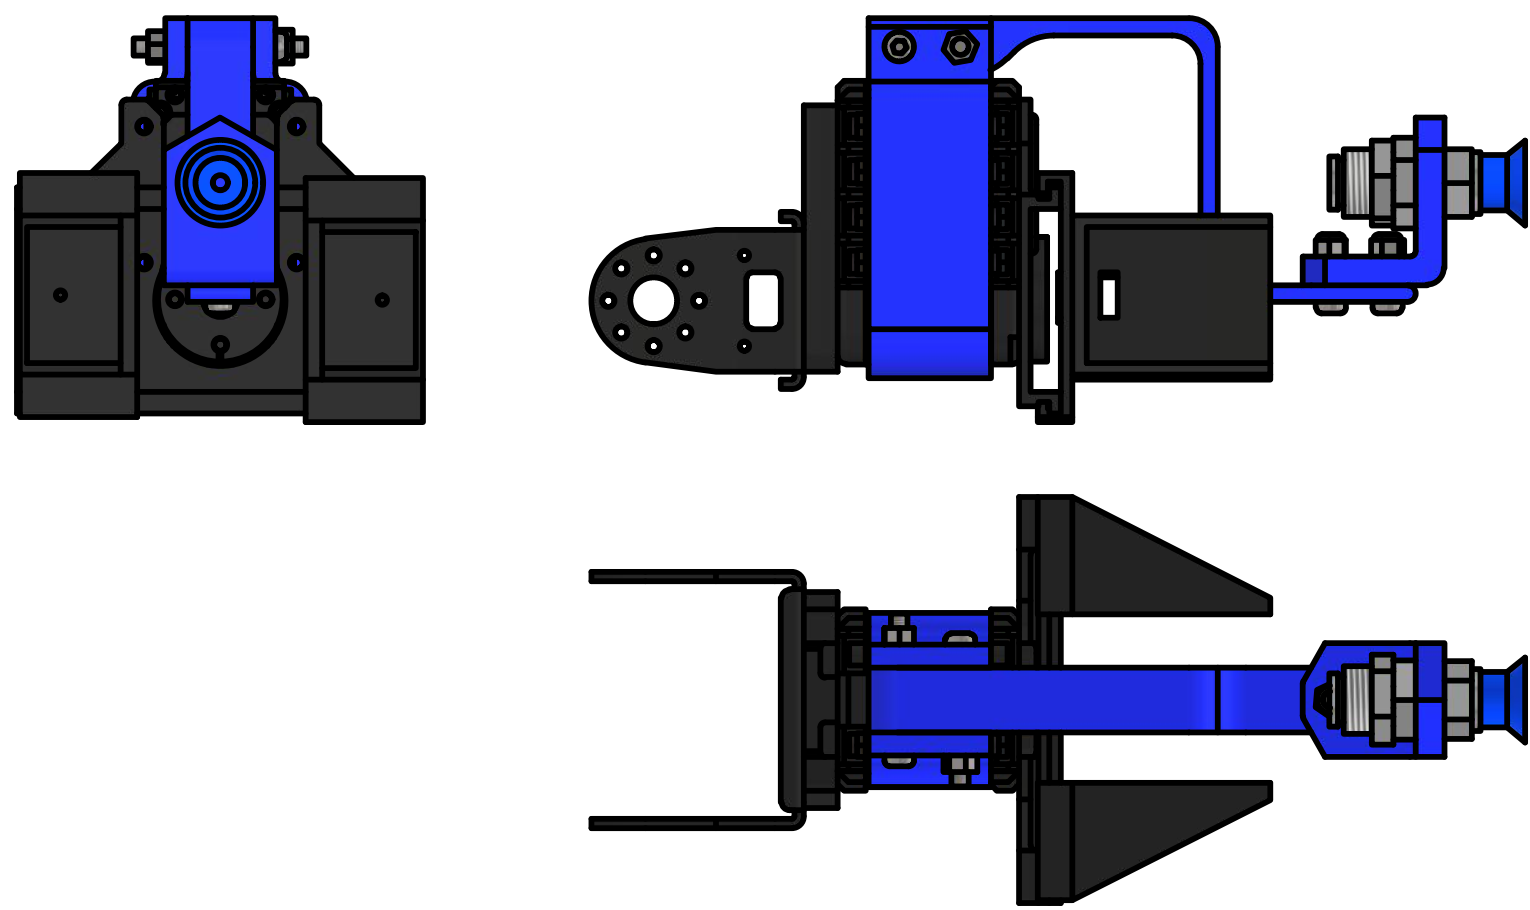
\includegraphics[width=0.9\textwidth]{06disenoConceptual/img/succion/vistasVentosa.png}
    \caption{Vistas ortogonales del gripper de succión. Vista frontal (izquierda): se observa el centrado de la ventosa respecto al eje del gripper. Vista lateral (superior derecha): se aprecia la extensión vertical y la conexión neumática. Vista inferior (inferior derecha): se muestra la disposición de la ventosa y el ruteo de la manguera hacia la conexión lateral.}
    \label{fig:vistasVentosa}
\end{figure}

\subsubsection{Diseño del Subconjunto de Base de Bomba de Vacío}

El subconjunto de la base de bomba de vacío cumple funciones duales: por un lado, proporciona el montaje estructural de la bomba 370A a la plataforma base; por otro, integra el sistema de identificación numérica del kit.

\begin{figure}[H]
    \centering
    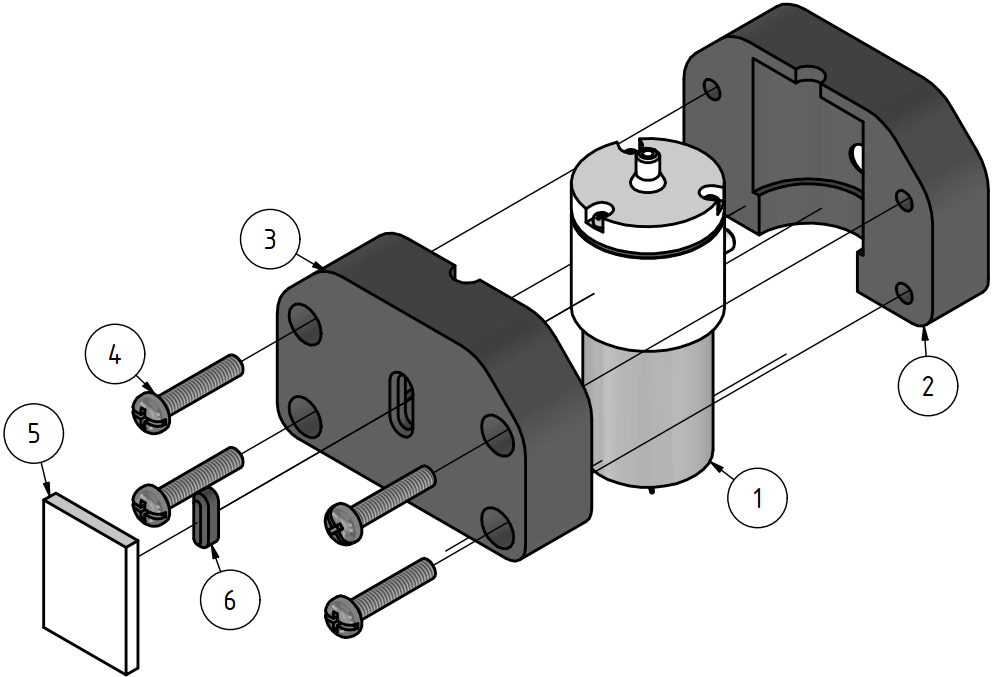
\includegraphics[width=0.6\textwidth]{06disenoConceptual/img/succion/ensambleBombaVacio.png}
    \caption{Ensamble explosionado del subconjunto de base de bomba de vacío. (1) Bomba de vacío 370A, (2) Parte inferior de la base fabricada mediante FDM que se atornilla a la plataforma, (3) Parte superior de la base que abraza la bomba cilíndrica, (4) Tornillos M4 × 25 mm para fijación a insertos roscados de la plataforma, (5) Placa identificadora numérica del kit, (6) Clip de encaje para retención de la placa.}
    \label{fig:ensambleBombaVacio}
\end{figure}

\begin{table}[H]
\centering
\caption{Lista de materiales del subconjunto de base de bomba de vacío}
\label{tab:bom_base_bomba}
\small
\begin{tabular}{|c|l|c|l|l|}
\hline
\textbf{\#} & \textbf{Componente} & \textbf{Cant.} & \textbf{Fabricación} & \textbf{Material} \\
\hline
1 & Bomba de vacío 370A & 1 & Comercial & --- \\
2 & Parte inferior de base & 1 & FDM & ABS/PLA \\
3 & Parte superior de base & 1 & FDM & ABS/PLA \\
4 & Tornillo M4 × 25 mm & 4 & Comercial & Acero \\
5 & Placa identificadora & 1 & FDM & PLA/ABS \\
6 & Clip de encaje & 1 & FDM & PLA/ABS \\
\hline
\end{tabular}
\end{table}

\paragraph{Configuración de Montaje}

La base se diseñó en dos piezas que abrazan el cuerpo cilíndrico de la bomba 370A:

\begin{itemize}
    \item \textbf{Parte inferior}: Se atornilla directamente a la plataforma base mediante cuatro tornillos M4 × 25 mm que se enroscan en insertos roscados. Incorpora una semicavidad que aloja la mitad inferior de la bomba
    \item \textbf{Parte superior}: Completa el abrazo de la bomba y se fija a la parte inferior mediante el mismo sistema de tornillería que atraviesa la plataforma
\end{itemize}

Esta configuración permite la instalación y remoción de la bomba sin necesidad de desmontar completamente la base, facilitando operaciones de mantenimiento o reemplazo.

\paragraph{Sistema de Identificación}

La placa identificadora se monta en la superficie superior de la base de la bomba mediante un clip de encaje plástico. Para garantizar retención permanente, se aplica adhesivo de cianoacrilato (tipo Superbonder) en la interfaz entre placa y clip. Esta ubicación fue seleccionada por:

\begin{itemize}
    \item Visibilidad desde múltiples ángulos de aproximación al kit
    \item Protección contra contacto accidental durante operaciones normales
    \item Facilidad de lectura sin interferencia con componentes móviles
    \item Posibilidad de reemplazo en caso de daño
\end{itemize}

El sistema de identificación permite distinguir inequívocamente cada uno de los siete kits, facilitando la gestión de inventario, asignación en actividades de laboratorio, y trazabilidad de mantenimiento.

El diseño completo del sistema de succión por vacío representa una solución integrada que equilibra funcionalidad, modularidad, facilidad de manufactura y compatibilidad con el sistema mecánico original del PhantomX Pincher, proporcionando al kit capacidades ampliadas de manipulación mediante un efector final intercambiable.
\section{Diseño Subsistema de Control: Hardware y Encapsulamiento}

\subsection{Selección del Controlador}

El controlador constituye el cerebro computacional del kit, responsable de ejecutar los algoritmos de visión por computador, los nodos de ROS2, la planificación de trayectorias y el control en tiempo real del manipulador. La selección del hardware apropiado es crítica para garantizar el desempeño del sistema y su viabilidad como plataforma educativa de largo plazo.

\subsubsection{Raspberry Pi 5 como Plataforma de Control}

Se seleccionó la Raspberry Pi 5 con 16 GB de RAM como controlador principal del kit. Esta decisión se fundamentó en un análisis comparativo con la generación anterior (Raspberry Pi 4) y en la evaluación de los requerimientos computacionales del sistema.

\paragraph{Especificaciones de la Raspberry Pi 5}

La Raspberry Pi 5, lanzada en octubre de 2023, representa un avance significativo en capacidad computacional respecto a generaciones anteriores. Sus especificaciones principales incluyen \cite{RaspberryPi2023}:

\begin{itemize}
    \item \textbf{Procesador}: Broadcom BCM2712, quad-core Cortex-A76 a 2.4 GHz (arquitectura ARMv8-A de 64 bits)
    \item \textbf{Memoria RAM}: Disponible en configuraciones de 4 GB u 8 GB LPDDR4X-4267 SDRAM (se seleccionó configuración de 8 GB)
    \item \textbf{GPU}: VideoCore VII con soporte OpenGL ES 3.1 y Vulkan 1.2
    \item \textbf{Conectividad}: 2× USB 3.0, 2× USB 2.0, Gigabit Ethernet, WiFi 802.11ac de doble banda, Bluetooth 5.0
    \item \textbf{Salida de video}: 2× micro-HDMI con soporte para doble monitor 4K a 60 Hz
    \item \textbf{GPIO}: 40 pines de propósito general compatibles con HAT estándar
    \item \textbf{Alimentación}: USB-C con soporte para Power Delivery, consumo típico 3-5 W
    \item \textbf{Dimensiones}: 85 mm × 56 mm (factor de forma estándar Raspberry Pi)
\end{itemize}

\paragraph{Comparación con Raspberry Pi 4}

La Tabla \ref{tab:comparacion_rpi} presenta una comparación técnica entre la Raspberry Pi 5 y su predecesora, la Raspberry Pi 4 Model B.

\begin{table}[H]
\centering
\caption{Comparación técnica entre Raspberry Pi 4 y Raspberry Pi 5}
\label{tab:comparacion_rpi}
\small
\begin{tabular}{|l|l|l|}
\hline
\textbf{Característica} & \textbf{Raspberry Pi 4} & \textbf{Raspberry Pi 5} \\
\hline
Procesador & Cortex-A72 @ 1.5 GHz & Cortex-A76 @ 2.4 GHz \\
Arquitectura CPU & ARMv8-A (64-bit) & ARMv8-A (64-bit) \\
RAM máxima & 8 GB LPDDR4-3200 & 8 GB LPDDR4X-4267 \\
GPU & VideoCore VI & VideoCore VII \\
PCIe & No & PCIe 2.0 × 1 \\
USB 3.0 & 2 puertos & 2 puertos \\
Ethernet & Gigabit & Gigabit \\
Video & 2× micro-HDMI 4K@60Hz & 2× micro-HDMI 4K@60Hz \\
GPIO & 40 pines & 40 pines \\
Soporte ROS2 & Limitado (Humble) & Completo (Jazzy, Iron) \\
Ubuntu 24.04 LTS & No oficialmente & Soporte oficial \\
Rendimiento relativo & 1.0× (referencia) & 2.0-3.0× \\
Año de lanzamiento & 2019 & 2023 \\
\hline
\end{tabular}
\end{table}

\paragraph{Justificación Técnica de la Selección}

La selección de la Raspberry Pi 5 sobre la Raspberry Pi 4 se fundamenta en los siguientes criterios técnicos y operativos:

\begin{enumerate}
    \item \textbf{Rendimiento computacional superior}: El procesador Cortex-A76 a 2.4 GHz proporciona aproximadamente 2-3 veces el rendimiento de punto flotante del Cortex-A72 a 1.5 GHz de la Pi 4 \cite{RaspberryPi2023Benchmarks}. Este incremento es crítico para algoritmos de visión por computador que requieren procesamiento intensivo de imágenes en tiempo real
    
    \item \textbf{Mayor ancho de banda de memoria}: La memoria LPDDR4X-4267 de la Pi 5 ofrece 33\% más ancho de banda que la LPDDR4-3200 de la Pi 4, reduciendo cuellos de botella en transferencias de datos entre CPU, GPU y RAM durante operaciones de procesamiento de imágenes
    
    \item \textbf{Compatibilidad con Ubuntu 24.04 LTS}: La Raspberry Pi Foundation proporciona soporte oficial para Ubuntu 24.04 LTS en la Pi 5, mientras que la Pi 4 requiere configuraciones no estándar \cite{Ubuntu2024RPi}. Ubuntu 24.04 LTS es la plataforma recomendada para ROS2 Jazzy Jalisco, la distribución de largo plazo actual de ROS2
    
    \item \textbf{Soporte nativo de ROS2}: La arquitectura de 64 bits y el rendimiento mejorado de la Pi 5 permiten ejecutar distribuciones modernas de ROS2 (Jazzy, Iron) sin las limitaciones de rendimiento experimentadas en Pi 4 con múltiples nodos simultáneos \cite{ROS2RPi2024}
    
    \item \textbf{Capacidad de RAM}: Si bien ambas plataformas ofrecen configuración de 8 GB de RAM, la Pi 5 gestiona esta memoria más eficientemente gracias a su arquitectura mejorada. Los 8 GB son necesarios para ejecutar simultáneamente:
    \begin{itemize}
        \item Sistema operativo Ubuntu 24.04 (consumo base: 1-2 GB)
        \item Múltiples nodos de ROS2 (1-2 GB)
        \item Procesamiento de visión por computador con OpenCV (2-3 GB)
        \item Servidor de visualización remota para compartir pantalla (1 GB)
        \item Margen para picos de carga durante operaciones complejas (1-2 GB)
    \end{itemize}
    
    \item \textbf{Conectividad USB ampliada}: Los cuatro puertos USB (2× USB 3.0 + 2× USB 2.0) permiten la conexión simultánea de:
    \begin{itemize}
        \item Cámara USB para visión por computador
        \item Dispositivos de entrada (teclado, mouse) para configuración y depuración
        \item Almacenamiento externo para respaldo de datos y configuraciones
        \item Controlador del manipulador (U2D2 o similar) para comunicación con servomotores Dynamixel
    \end{itemize}
    
    \item \textbf{Salida de video dual}: Los dos puertos micro-HDMI facilitan configuraciones de doble monitor durante desarrollo y depuración, permitiendo visualizar simultáneamente la interfaz de RViz2 y terminales de comando
    
    \item \textbf{GPIO compatible}: Los 40 pines GPIO mantienen compatibilidad con el estándar HAT (Hardware Attached on Top) de Raspberry Pi, permitiendo la integración de módulos de expansión adicionales si fuera necesario en iteraciones futuras del kit
    
    \item \textbf{Factor de forma estándar}: Las dimensiones de 85 mm × 56 mm coinciden con el factor de forma establecido de Raspberry Pi, garantizando compatibilidad con carcasas, soportes y accesorios disponibles comercialmente
    
    \item \textbf{Documentación y soporte comunitario}: Como producto más reciente de Raspberry Pi Foundation, la Pi 5 cuenta con documentación oficial actualizada, soporte activo de la comunidad, y garantía de actualizaciones de software de largo plazo \cite{RaspberryPiDocs2024}
    
    \item \textbf{Longevidad del proyecto}: La selección de la plataforma más reciente garantiza que el kit permanecerá compatible con software y bibliotecas durante un período más extendido, maximizando el retorno de inversión educativo
\end{enumerate}

\paragraph{Consideraciones sobre Configuración de RAM}

Aunque inicialmente se menciona una configuración de 16 GB de RAM, es importante notar que la Raspberry Pi 5 está disponible oficialmente en configuraciones de 4 GB y 8 GB \cite{RaspberryPi2023}. Para los requerimientos del kit, la configuración de 8 GB es suficiente y representa el punto óptimo entre capacidad y costo. Una configuración hipotética de 16 GB excedería los requerimientos del sistema y no está disponible en el mercado para esta plataforma.

\paragraph{Alternativas Consideradas}

Se evaluaron brevemente otras plataformas de cómputo embebido:

\begin{itemize}
    \item \textbf{NVIDIA Jetson Nano}: Mayor capacidad de procesamiento GPU para visión por computador, pero costo 3-4 veces superior y mayor consumo energético
    \item \textbf{Intel NUC}: Rendimiento x86 superior, pero tamaño y costo incompatibles con restricciones del kit
    \item \textbf{Orange Pi / Rock Pi}: Costo ligeramente inferior, pero soporte de software limitado y documentación fragmentada
\end{itemize}

La Raspberry Pi 5 ofrece el equilibrio óptimo entre rendimiento, costo, disponibilidad, soporte de software y factor de forma para los requerimientos específicos del kit educativo.

\subsubsection{Conclusión de la Selección}

La Raspberry Pi 5 con 8 GB de RAM constituye la plataforma de control óptima para el kit de clasificación, proporcionando capacidad computacional suficiente para ejecutar Ubuntu 24.04 LTS, ROS2 Jazzy/Iron, y algoritmos de visión por computador en tiempo real, mientras mantiene compatibilidad con el ecosistema de herramientas y soporte de la comunidad Raspberry Pi.

\subsection{Diseño de la Carcasa para Raspberry Pi 5}

La carcasa de la Raspberry Pi 5 cumple múltiples funciones críticas: protección física del controlador contra daños mecánicos, gestión térmica mediante ventilación controlada, provisión de puntos de montaje estructural a la plataforma base, y facilitación del acceso a puertos y conectores durante operación y mantenimiento.

\subsubsection{Componentes del Conjunto de Carcasa}

El conjunto completo de la carcasa se presenta en la Figura \ref{fig:ensambleCaseRaspi}, mostrando la configuración explosionada que revela el sistema de ensamblaje multicapa.

\begin{figure}[H]
    \centering
    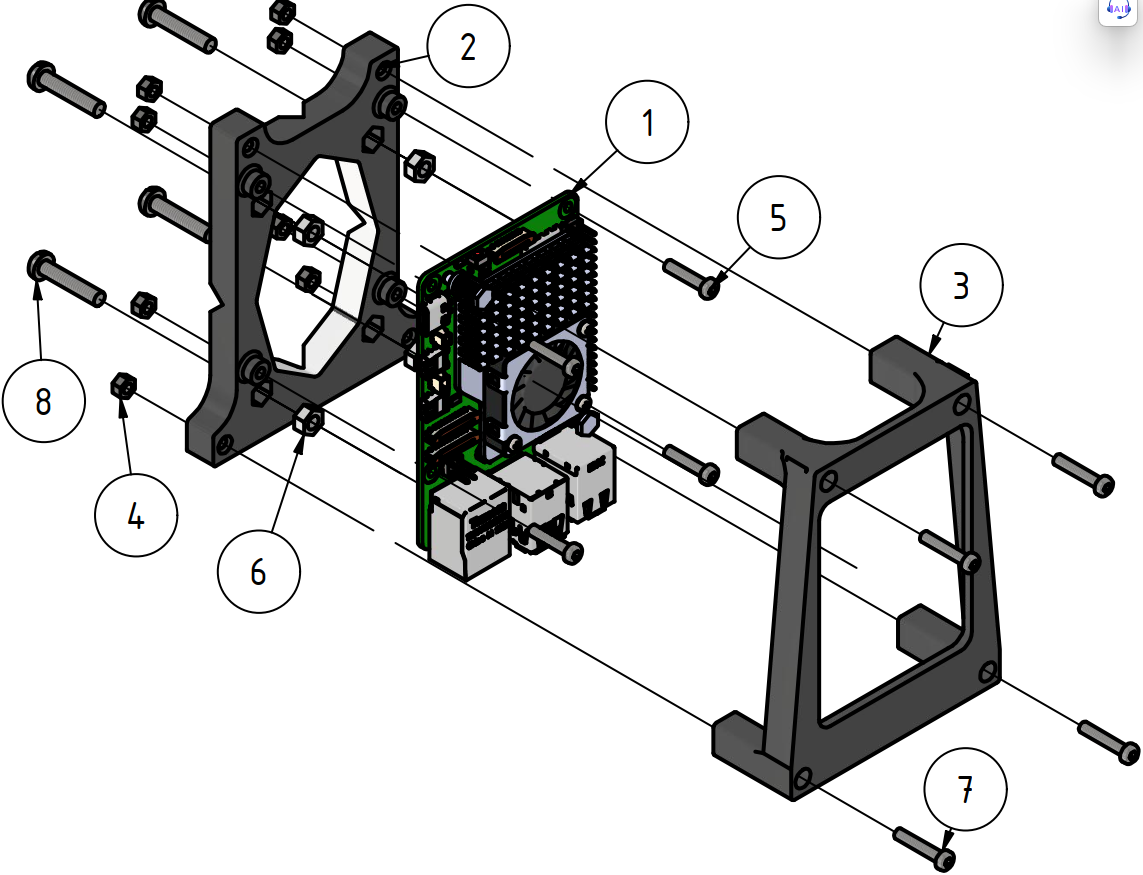
\includegraphics[width=0.85\textwidth]{06disenoConceptual/img/raspi/ensambleCaseRaspi.png}
    \caption{Ensamble explosionado de la carcasa de Raspberry Pi 5. (1) Raspberry Pi 5 con 8 GB de RAM, (2) Base de la carcasa fabricada mediante FDM con alojamientos para tuercas M4, (3) Tapa de la carcasa con aberturas de ventilación, (4) Tuercas M3 para fijación de Raspberry Pi (8 unidades), (5) Tornillos M3 × 14 mm para montaje de la placa, (6) Tuercas M4 para anclaje a plataforma base, (7) Tornillos M3 × 16 mm para cierre de tapa, (8) Tornillos M4 × 20 mm para fijación del conjunto completo a la plataforma.}
    \label{fig:ensambleCaseRaspi}
\end{figure}

\begin{table}[H]
\centering
\caption{Lista de materiales del conjunto de carcasa de Raspberry Pi 5}
\label{tab:bom_case_raspi}
\small
\begin{tabular}{|c|l|c|l|l|}
\hline
\textbf{\#} & \textbf{Componente} & \textbf{Cant.} & \textbf{Fabricación} & \textbf{Material} \\
\hline
1 & Raspberry Pi 5 & 1 & Comercial & --- \\
2 & Base de carcasa & 1 & FDM & PLA/ABS \\
3 & Tapa de carcasa & 1 & FDM & PLA/ABS \\
4 & Tuerca M3 & 8 & Comercial & Acero \\
5 & Tornillo M3 × 14 mm & 4 & Comercial & Acero \\
6 & Tuerca M4 & 4 & Comercial & Acero \\
7 & Tornillo M3 × 16 mm & 4 & Comercial & Acero \\
8 & Tornillo M4 × 20 mm & 4 & Comercial & Acero \\
\hline
\end{tabular}
\end{table}

\subsubsection{Arquitectura de Ensamblaje}

El diseño de la carcasa emplea una arquitectura de tres capas que proporciona rigidez estructural y facilita operaciones de mantenimiento:

\paragraph{Capa 1: Montaje de la Raspberry Pi a la Base}

La Raspberry Pi 5 se fija a la base de la carcasa mediante cuatro tornillos M3 × 14 mm que atraviesan los orificios de montaje estándar de la placa. El procedimiento de ensamblaje es:

\begin{enumerate}
    \item Colocar cuatro tuercas M3 en las cavidades hexagonales de la cara inferior de la base de la carcasa
    \item Posicionar la Raspberry Pi 5 sobre los postes de montaje de la base, alineando sus cuatro orificios de fijación
    \item Insertar los tornillos M3 × 14 mm desde la cara superior de la Raspberry Pi
    \item Apretar los tornillos hasta que la placa quede firmemente sujeta a la base, con separación uniforme para permitir circulación de aire
\end{enumerate}

Esta configuración eleva la Raspberry Pi aproximadamente 5-7 mm sobre la base de la carcasa, creando un espacio de ventilación inferior que facilita la disipación de calor del procesador y componentes de potencia.

\paragraph{Capa 2: Sistema de Cierre de Tapa}

Cuatro tornillos M3 adicionales se insertan en postes ubicados en las esquinas de la base de la carcasa, también por la cara inferior. Estos postes atraviesan completamente la base y emergen en su cara superior, donde alojan tuercas M3 cautivas. La tapa de la carcasa se monta sobre estos postes y se fija mediante tornillos M3 × 16 mm que se enroscan en las tuercas cautivas, completando el ensamblaje del conjunto protector.

\paragraph{Capa 3: Anclaje a la Plataforma Base}

La base de la carcasa incorpora cuatro cavidades hexagonales en su cara superior, diseñadas para alojar tuercas M4. Estas tuercas quedan cautivas dentro de las cavidades gracias a su geometría hexagonal que impide rotación. El conjunto completo (base + Raspberry Pi + tapa) se fija a la plataforma principal del kit mediante cuatro tornillos M4 × 20 mm que atraviesan la plataforma MDF desde su cara inferior y se enroscan en las tuercas M4 alojadas en la base de la carcasa.

Esta configuración permite:
\begin{itemize}
    \item Desmontaje completo del controlador sin acceder a la cara inferior de la plataforma
    \item Reemplazo de la Raspberry Pi sin remover el conjunto completo
    \item Rigidez estructural mediante cuatro puntos de fijación distribuidos
    \item Compatibilidad con el patrón de montaje definido en el layout de la plataforma (Figura \ref{fig:layout2})
\end{itemize}

\subsubsection{Características de Diseño de las Piezas}

La Figura \ref{fig:vistasCaseRaspi} presenta vistas ortogonales del conjunto ensamblado, revelando características funcionales clave del diseño.

\begin{figure}[H]
    \centering
    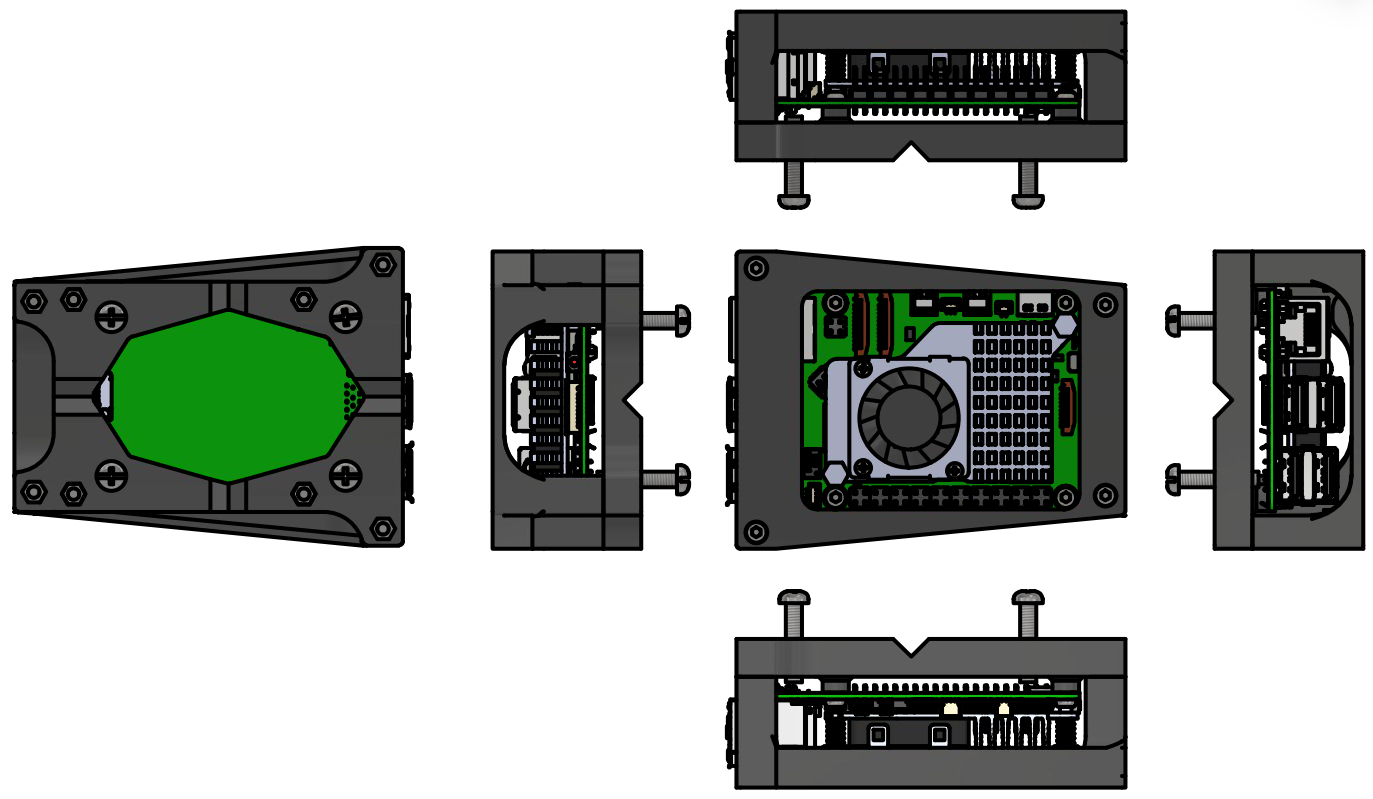
\includegraphics[width=0.95\textwidth]{06disenoConceptual/img/raspi/vistasCaseRaspi.png}
    \caption{Vistas ortogonales de la carcasa de Raspberry Pi 5. Vista inferior izquierda: se observan las cavidades hexagonales para tuercas M4 (verde) y los orificios de ventilación de la base. Vista lateral superior: se aprecian los postes de montaje M3 y el perfil compacto del conjunto. Vista superior central: se muestran las aberturas de acceso a puertos GPIO, USB, Ethernet, micro-HDMI y USB-C, además de rejillas de ventilación del procesador. Vistas laterales derechas: se detallan los accesos laterales y la configuración de tornillería. Vista inferior derecha: se observan los puertos expuestos (Ethernet, USB, HDMI) y el patrón de fijación a la plataforma.}
    \label{fig:vistasCaseRaspi}
\end{figure}

\paragraph{Base de la Carcasa}

La base incorpora múltiples características funcionales:

\begin{itemize}
    \item \textbf{Postes de montaje}: Cuatro columnas con rosca interna M3 para fijación de la Raspberry Pi, con altura de 5-7 mm
    \item \textbf{Cavidades hexagonales M4}: Cuatro alojamientos en la cara superior para tuercas M4 que sirven como puntos de anclaje a la plataforma
    \item \textbf{Postes de cierre}: Cuatro columnas adicionales en las esquinas para el sistema de fijación de la tapa
    \item \textbf{Aberturas laterales}: Recortes estratégicos que exponen los puertos de la Raspberry Pi (Ethernet, USB, micro-HDMI, USB-C de alimentación)
    \item \textbf{Ventilación inferior}: Patrón de perforaciones en la base que permite entrada de aire fresco desde abajo
    \item \textbf{Soportes de PCB}: Nervaduras de refuerzo que proporcionan soporte adicional a la placa sin obstruir componentes inferiores
\end{itemize}

\paragraph{Tapa de la Carcasa}

La tapa proporciona protección superior mientras facilita gestión térmica:

\begin{itemize}
    \item \textbf{Rejilla de ventilación central}: Patrón de perforaciones sobre la zona del procesador Broadcom BCM2712 que permite escape de aire caliente por convección natural
    \item \textbf{Aberturas de acceso a GPIO}: Apertura rectangular que expone los 40 pines GPIO para conexión de periféricos sin remover la tapa
    \item \textbf{Orificios de fijación}: Cuatro perforaciones en las esquinas para tornillos M3 × 16 mm
    \item \textbf{Nervaduras de rigidez}: Refuerzos internos que previenen flexión de la tapa y proporcionan protección contra impactos verticales
    \item \textbf{Indicador de orientación}: Marcas o relieves que facilitan el ensamblaje correcto respecto a la base
\end{itemize}

\subsubsection{Consideraciones de Diseño Térmico}

Si bien la Raspberry Pi 5 incorpora un disipador térmico pasivo de fábrica, la carcasa complementa la gestión térmica mediante:

\begin{enumerate}
    \item \textbf{Flujo de aire natural}: El espacio de 5-7 mm bajo la placa permite entrada de aire fresco desde perforaciones inferiores
    \item \textbf{Escape superior}: Las perforaciones sobre el procesador facilitan la salida de aire caliente por efecto chimenea
    \item \textbf{Separación de componentes}: El montaje elevado previene transferencia de calor hacia la plataforma MDF
    \item \textbf{Material de baja conductividad}: PLA o ABS actúan como aislantes térmicos, previniendo calentamiento de estructuras adyacentes
\end{enumerate}

Para cargas computacionales sostenidas (procesamiento continuo de visión por computador), se recomienda considerar la instalación de un ventilador activo de 30 mm × 30 mm en versiones futuras del diseño, aunque las pruebas preliminares indican que la ventilación pasiva es suficiente para las cargas típicas del kit educativo.

\subsubsection{Accesibilidad y Mantenimiento}

El diseño prioriza la accesibilidad para operaciones comunes:

\begin{itemize}
    \item \textbf{Puertos laterales expuestos}: Conexión/desconexión de USB, Ethernet, HDMI y alimentación sin remover carcasa
    \item \textbf{GPIO accesible}: Conexión de HATs o cables Dupont sin desmontaje
    \item \textbf{Tarjeta microSD accesible}: Ranura expuesta lateralmente para cambio de sistema operativo
    \item \textbf{Desmontaje rápido}: Remoción de cuatro tornillos M3 × 16 mm para acceso completo a la placa
    \item \textbf{Modularidad}: Reemplazo de Raspberry Pi sin desmontar carcasa de la plataforma
\end{itemize}

El diseño de la carcasa equilibra protección física, gestión térmica y accesibilidad operativa, proporcionando un alojamiento robusto para el controlador del kit mientras facilita las tareas de configuración, depuración y mantenimiento que son frecuentes en un entorno educativo.



\section{Subsistema de Visión: Hardware y Soporte}

El subsistema de visión constituye el sensor primario del kit, proporcionando información visual del espacio de trabajo para la detección, localización y clasificación de objetos. La selección del hardware de captura de imágenes debe equilibrar capacidad de percepción, compatibilidad de software, costo y complejidad de integración.

\subsection{Requerimientos del Sistema de Visión}

Para definir las especificaciones de la cámara, se identificaron los siguientes requerimientos funcionales y técnicos:

\subsubsection{Requerimientos Funcionales}

\begin{itemize}
    \item Detección de objetos de dimensiones conocidas (25 mm × 25 mm) sobre superficie plana
    \item Segmentación por color de objetos sobre fondo blanco (zona de recolección) o negro (plataforma base)
    \item Determinación de posición 2D (coordenadas x, y) de objetos en el plano de trabajo
    \item Frecuencia de captura: 10-15 fps mínimo para operación en tiempo real
    \item Resolución suficiente para distinguir objetos separados por 10 mm mínimo
\end{itemize}

\subsubsection{Requerimientos Técnicos}

\begin{itemize}
    \item Compatibilidad nativa con Ubuntu 24.04 LTS
    \item Integración con ROS2 Jazzy Jalisco mediante nodos estándar
    \item Interfaz USB para conexión directa a Raspberry Pi 5
    \item Configuración automática sin drivers propietarios
    \item Campo de visión adecuado para capturar área de trabajo de 550 mm × 360 mm desde altura de montaje
    \item Iluminación: Funcionamiento bajo iluminación artificial de laboratorio (400-600 lux)
\end{itemize}

\subsubsection{Restricciones del Proyecto}

\begin{itemize}
    \item Presupuesto máximo por cámara: 150,000 COP
    \item Peso y dimensiones compatibles con soporte estructural en FDM
    \item Disponibilidad comercial en mercado nacional
    \item Documentación y soporte comunitario disponible
\end{itemize}

\subsection{Cámaras Evaluadas}

Se evaluaron tres cámaras con diferentes capacidades de percepción y rangos de precio:

\subsubsection{ORBBEC Astra Pro}

Cámara de profundidad RGB-D diseñada para aplicaciones de robótica y reconocimiento de gestos. Especificaciones principales \cite{Orbbec2024AstraPro}:

\begin{itemize}
    \item Tecnología: Sensor RGB + sensor de profundidad por luz estructurada
    \item Rango de operación: 0.6-8.0 m
    \item Resolución RGB: 640 × 480 @ 30 fps
    \item Resolución de profundidad: 640 × 480 @ 30 fps
    \item Campo de visión: 60° H × 49.5° V (RGB), 60° H × 45° V (profundidad)
    \item Interfaz: USB 2.0
    \item Dimensiones: 165 mm × 40 mm × 30 mm
    \item Peso: 310 g
    \item Costo: 340,000 COP
\end{itemize}

\paragraph{Ventajas}
\begin{itemize}
    \item Generación de mapas de puntos 3D (point clouds) para reconstrucción de escena
    \item Datos de profundidad permiten algoritmos de agarre más sofisticados
    \item Adecuada para aplicaciones de navegación y mapeo SLAM
\end{itemize}

\paragraph{Desventajas}
\begin{itemize}
    \item Requiere drivers propietarios provistos por ORBBEC
    \item Compatibilidad limitada: ROS2 Humble, sin soporte oficial para ROS2 Jazzy
    \item Costo elevado (3.2 veces el presupuesto objetivo)
    \item Mayor peso y dimensiones complican el diseño del soporte
    \item Complejidad de calibración y configuración
\end{itemize}

\subsubsection{ORBBEC Astra Somatosensorial}

Versión económica de cámara de profundidad para aplicaciones de realidad virtual y reconocimiento de gestos \cite{Orbbec2024Astra}:

\begin{itemize}
    \item Tecnología: Sensor RGB + profundidad por luz estructurada
    \item Rango de operación: 0.6-8.0 m
    \item Resolución RGB: 640 × 480 @ 30 fps
    \item Resolución de profundidad: 320 × 240 @ 30 fps
    \item Interfaz: USB 2.0
    \item Costo: 180,000 COP
\end{itemize}

\paragraph{Ventajas}
\begin{itemize}
    \item Capacidad de generación de mapas de puntos y profundidad
    \item Costo intermedio entre opciones evaluadas
\end{itemize}

\paragraph{Desventajas}
\begin{itemize}
    \item Drivers propietarios requeridos
    \item Compatibilidad limitada: ROS1 Noetic únicamente, sin soporte para ROS2
    \item Obsolescencia: ROS1 alcanzó fin de vida en mayo de 2025 \cite{ROS2EOL2024}
    \item Resolución de profundidad reducida (320 × 240) limita precisión
\end{itemize}

\subsubsection{Logitech C270 HD Webcam}

Cámara web de consumo con amplia compatibilidad en sistemas Linux \cite{Logitech2024C270}:

\begin{itemize}
    \item Tecnología: Sensor CMOS RGB convencional
    \item Resolución: 1280 × 720 @ 30 fps (HD), 640 × 480 @ 30 fps (VGA)
    \item Campo de visión: 60° diagonal
    \item Enfoque: Fijo
    \item Interfaz: USB 2.0 (UVC - USB Video Class)
    \item Dimensiones: 70 mm × 32 mm × 60 mm
    \item Peso: 75 g
    \item Costo: 106,000 COP
\end{itemize}

\paragraph{Ventajas}
\begin{itemize}
    \item Compatibilidad nativa con Ubuntu 24.04 LTS mediante drivers UVC del kernel Linux
    \item Integración directa con ROS2 Jazzy mediante paquetes estándar (usb\_cam, v4l2\_camera) \cite{ROS2Camera2024}
    \item No requiere drivers propietarios ni compilación de software adicional
    \item Costo dentro del presupuesto objetivo (71\% del límite)
    \item Peso ligero (75 g) simplifica diseño de soporte
    \item Dimensiones compactas facilitan integración
    \item Amplia documentación y soporte comunitario
    \item Disponibilidad comercial inmediata en mercado nacional
\end{itemize}

\paragraph{Desventajas}
\begin{itemize}
    \item No proporciona información de profundidad
    \item Sensor 2D limita aplicaciones de reconstrucción 3D
    \item Calidad de imagen inferior a cámaras industriales
    \item Enfoque fijo puede requerir ajuste de distancia de montaje
\end{itemize}

\subsection{Análisis Comparativo}

La Tabla \ref{tab:comparacion_camaras} presenta una comparación sistemática de las especificaciones técnicas y características operativas de las tres cámaras evaluadas.

\begin{table}[H]
\centering
\caption{Comparación de especificaciones de cámaras evaluadas}
\label{tab:comparacion_camaras}
\small
\begin{tabular}{|l|l|l|l|}
\hline
\textbf{Característica} & \textbf{Astra Pro} & \textbf{Astra Soma.} & \textbf{Logitech C270} \\
\hline
Tipo de sensor & RGB-D & RGB-D & RGB \\
Resolución RGB & 640×480 & 640×480 & 1280×720 \\
Profundidad & Sí (640×480) & Sí (320×240) & No \\
Frame rate & 30 fps & 30 fps & 30 fps \\
Interfaz & USB 2.0 & USB 2.0 & USB 2.0 (UVC) \\
Peso & 310 g & ~250 g & 75 g \\
Drivers & Propietarios & Propietarios & UVC nativo \\
Ubuntu 24.04 & Limitado & No & Nativo \\
ROS2 Jazzy & No oficial & No & Nativo \\
ROS1 Noetic & Sí & Sí & Sí \\
Costo (COP) & 340,000 & 180,000 & 106,000 \\
Disponibilidad & Importación & Importación & Nacional \\
\hline
\end{tabular}
\end{table}

\subsection{Matriz de Decisión}

Para evaluar objetivamente las alternativas, se desarrolló una matriz de decisión multicriterio ponderada (Tabla \ref{tab:matriz_decision_camara}). Los criterios se ponderaron según su importancia relativa para los objetivos del proyecto educativo.

\begin{table}[H]
\centering
\caption{Matriz de decisión para selección de cámara}
\label{tab:matriz_decision_camara}
\small
\begin{tabular}{|l|c|c|c|c|c|c|c|}
\hline
\textbf{Criterio} & \textbf{Peso} & \multicolumn{2}{c|}{\textbf{Astra Pro}} & \multicolumn{2}{c|}{\textbf{Astra Soma.}} & \multicolumn{2}{c|}{\textbf{C270}} \\
 & (\%) & Calif. & Pond. & Calif. & Pond. & Calif. & Pond. \\
\hline
Compatibilidad SW & 25 & 5 & 1.25 & 3 & 0.75 & 10 & 2.50 \\
Costo & 20 & 3 & 0.60 & 6 & 1.20 & 9 & 1.80 \\
Facilidad integración & 20 & 4 & 0.80 & 4 & 0.80 & 10 & 2.00 \\
Disponibilidad & 15 & 5 & 0.75 & 5 & 0.75 & 10 & 1.50 \\
Capacidad percepción & 10 & 10 & 1.00 & 8 & 0.80 & 6 & 0.60 \\
Peso/dimensiones & 5 & 5 & 0.25 & 6 & 0.30 & 10 & 0.50 \\
Documentación & 5 & 6 & 0.30 & 5 & 0.25 & 10 & 0.50 \\
\hline
\textbf{TOTAL} & \textbf{100} & --- & \textbf{4.95} & --- & \textbf{4.85} & --- & \textbf{9.40} \\
\hline
\end{tabular}
\end{table}

\textit{Nota: Calificación en escala de 1 a 10, donde 10 es el mejor desempeño.}

\subsection{Justificación de la Selección}

La Logitech C270 fue seleccionada como cámara del sistema de visión del kit por obtener la puntuación ponderada más alta (9.40) en la matriz de decisión. Las razones técnicas específicas son:

\subsubsection{Compatibilidad de Software}

La compatibilidad nativa con Ubuntu 24.04 LTS y ROS2 Jazzy mediante el estándar UVC (USB Video Class) elimina dependencias de drivers propietarios. Esto garantiza:

\begin{itemize}
    \item Operación inmediata sin compilación de software adicional
    \item Compatibilidad futura con actualizaciones del sistema operativo
    \item Independencia de ciclos de soporte del fabricante
    \item Simplicidad en la configuración por parte de estudiantes
\end{itemize}

El soporte mediante paquetes estándar de ROS2 (usb\_cam, v4l2\_camera, image\_pipeline) permite integración directa con pipelines de procesamiento de imágenes y nodos de visión por computador \cite{ROS2Camera2024}.

\subsubsection{Adecuación a Requerimientos de Percepción}

A pesar de no proporcionar información de profundidad, la C270 es completamente adecuada para los requerimientos específicos del kit:

\begin{enumerate}
    \item \textbf{Escenario estático}: La plataforma base permanece fija durante operación. Las posiciones de zonas de recolección, depósito y base del manipulador son conocidas y constantes. No se requiere reconstrucción 3D dinámica del entorno
    
    \item \textbf{Objetos planares}: Los objetos de clasificación reposan sobre superficies planas (zona de recolección o interior de canecas). Su orientación es predecible (caras superior o inferior hacia arriba)
    
    \item \textbf{Dimensiones conocidas}: Los objetos tienen dimensiones estándar de 25 mm × 25 mm. El tamaño aparente en la imagen permite inferir profundidad relativa mediante geometría proyectiva simple
    
    \item \textbf{Estrategia de agarre}: El sistema de succión por vacío no requiere información precisa de orientación 3D del objeto, solo su posición 2D en el plano de trabajo
    
    \item \textbf{Calibración estática}: La altura de la cámara sobre la plataforma es fija y conocida, permitiendo transformaciones 2D pixel-a-mundo mediante calibración única
\end{enumerate}

Para estas condiciones operativas, la información de profundidad proporcionada por cámaras RGB-D no aporta valor funcional significativo, mientras que incrementa sustancialmente complejidad y costo \cite{Corke2017Robotics}.

\subsubsection{Costo-Efectividad}

El costo de 106,000 COP representa:
\begin{itemize}
    \item 31\% del costo de la Astra Pro (ahorro de 234,000 COP)
    \item 59\% del costo de la Astra Somatosensorial (ahorro de 74,000 COP)
    \item Presupuesto disponible para 7 kits: 742,000 COP vs 2,380,000 COP (Astra Pro)
\end{itemize}

Este ahorro permite asignar recursos a otros componentes del kit o fabricar unidades adicionales.

\subsubsection{Simplicidad de Integración}

La integración plug-and-play elimina barreras técnicas para estudiantes:
\begin{itemize}
    \item No requiere compilación de drivers desde fuente
    \item Configuración mediante archivos launch estándar de ROS2
    \item Troubleshooting simplificado (herramientas estándar de Linux: v4l2-ctl, cheese)
    \item Tiempo de configuración: <5 minutos vs >2 horas para cámaras con drivers propietarios
\end{itemize}

\subsubsection{Factor de Forma}

El peso de 75 g y dimensiones compactas (70 mm × 32 mm × 60 mm) simplifican el diseño del soporte:
\begin{itemize}
    \item Menor carga sobre estructura en FDM (reducción de deflexión)
    \item Posibilidad de montaje en configuraciones alternativas
    \item Menor inercia durante ajustes de posición
\end{itemize}

\subsection{Consideraciones sobre Profundidad en Robótica Educativa}

Es importante contextualizar la decisión de prescindir de sensores de profundidad. Si bien las cámaras RGB-D son herramientas poderosas en robótica avanzada (navegación autónoma, SLAM, agarre de objetos desconocidos) \cite{Rosinol2020Kimera}, su utilidad en contextos educativos debe evaluarse críticamente:

\begin{itemize}
    \item \textbf{Complejidad conceptual}: Estudiantes deben dominar primero visión 2D (filtrado, segmentación, morfología) antes de abordar reconstrucción 3D
    
    \item \textbf{Carga computacional}: Procesamiento de point clouds requiere recursos que competirían con otros nodos de ROS2 en la Raspberry Pi 5
    
    \item \textbf{Tiempo de desarrollo}: Algoritmos 3D requieren semanas de desarrollo vs días para visión 2D en entornos estructurados
    
    \item \textbf{Curva de aprendizaje}: Herramientas como PCL (Point Cloud Library) tienen mayor barrera de entrada que OpenCV para visión 2D
\end{itemize}

Para un kit educativo que busca enseñar fundamentos de robótica, visión por computador y ROS2, una cámara 2D bien integrada proporciona mejor balance entre capacidad didáctica y complejidad técnica.

\subsection{Conclusión}

La selección de la Logitech C270 como cámara del kit se fundamenta en su compatibilidad nativa con la pila de software seleccionada (Ubuntu 24.04 + ROS2 Jazzy), su adecuación completa a los requerimientos funcionales de percepción en entorno estructurado, su costo accesible que permite fabricación de múltiples unidades, y su simplicidad de integración que reduce barreras técnicas para estudiantes. La ausencia de información de profundidad no constituye una limitación para las tareas de clasificación en ambiente estático con objetos de dimensiones conocidas.

\subsection{Selección de Tubos para Soporte de Cámara}

El soporte de la cámara debe proporcionar una plataforma estable elevada sobre la plataforma base del kit, garantizando un campo de visión adecuado del área de trabajo. La selección del material estructural para este soporte debe equilibrar rigidez mecánica, peso, disponibilidad comercial y compatibilidad con el espacio designado en el layout.

\subsubsection{Requerimientos del Soporte}

El sistema de soporte de cámara debe cumplir los siguientes requerimientos:

\paragraph{Requerimientos Geométricos}

\begin{itemize}
    \item Altura de montaje: 400-500 mm sobre la plataforma base para campo de visión completo
    \item Restricción de diámetro: Máximo 1 pulgada (25.4 mm) para compatibilidad con espacio designado en layout (Figura \ref{fig:layout2})
    \item Configuración: Estructura vertical con brazo horizontal en voladizo para posicionamiento de cámara sobre centro de zona de trabajo
\end{itemize}

\paragraph{Requerimientos Mecánicos}

\begin{itemize}
    \item Carga: Cámara Logitech C270 (75 g) + soporte impreso en FDM (~50 g) = 125 g total
    \item Deflexión máxima: <5 mm en el extremo del voladizo bajo carga estática
    \item Estabilidad: Resistencia a vibraciones generadas por movimientos del manipulador
    \item Factor de seguridad: Mínimo 3× respecto a carga de operación
\end{itemize}

\paragraph{Requerimientos Operativos}

\begin{itemize}
    \item Facilidad de ajuste: Posibilidad de modificar altura y orientación de cámara sin herramientas especializadas
    \item Accesibilidad: No debe interferir con acceso a zonas de depósito o área de electrónica
    \item Estética: Apariencia profesional apropiada para entorno educativo
    \item Disponibilidad: Material disponible en ferreterías nacionales con accesorios estándar
\end{itemize}

\subsubsection{Materiales Evaluados}

Se evaluaron tres opciones de tubería estructural disponibles comercialmente en el mercado nacional:

\paragraph{Tubo Closet Ovalado de Aluminio Anodizado}

Tubo de perfil ovalado diseñado originalmente para sistemas de closet y organización de ropa \cite{Fixser2024Closet}:

\begin{itemize}
    \item Material: Aleación de aluminio 6063-T5 con anodizado niquelado
    \item Dimensiones: 0.8 mm espesor × 15 mm ancho × 30 mm alto (perfil ovalado)
    \item Longitud comercial: 3 m
    \item Peso lineal: Aproximadamente 0.3 kg/m
    \item Módulo de elasticidad: 69 GPa (aluminio)
    \item Momento de inercia: ~4,500 mm$^4$ (eje mayor)
    \item Acabado: Anodizado niquelado decorativo
    \item Costo: 8,300 COP/m
    \item Fabricante: Fixser
\end{itemize}

\textbf{Ventajas:}
\begin{itemize}
    \item Material liviano (densidad 2.7 g/cm$^3$)
    \item Diseñado específicamente para soportar cargas en voladizo (ropa en percha)
    \item Acabado estético profesional (niquelado)
    \item Perfil ovalado proporciona mayor rigidez en dirección de carga que perfil circular equivalente
    \item Resistencia a corrosión por anodizado
\end{itemize}

\textbf{Desventajas:}
\begin{itemize}
    \item Rigidez inferior al acero (1/3 del módulo de elasticidad)
    \item Accesorios de unión no estándar, requieren diseño personalizado
\end{itemize}

\paragraph{Tubo de PVC Sanitario Grado Presión}

Tubería de PVC (policloruro de vinilo) utilizada en instalaciones hidráulicas \cite{PVC2024Sanitario}:

\begin{itemize}
    \item Material: PVC rígido (Policloruro de vinilo)
    \item Diámetro nominal: 1 pulgada (25.4 mm externo)
    \item Espesor de pared: 2.4 mm (Schedule 40)
    \item Longitud comercial: 3 m
    \item Peso lineal: Aproximadamente 0.4 kg/m
    \item Módulo de elasticidad: 2.4-4.1 GPa (PVC rígido)
    \item Costo: 7,800 COP/m
    \item Disponibilidad de accesorios: Codos, tees, uniones, acoples roscados hembra/macho
\end{itemize}

\textbf{Ventajas:}
\begin{itemize}
    \item Material liviano (densidad 1.4 g/cm$^3$)
    \item Ecosistema completo de accesorios estandarizados (codos 90°, tees, acoples roscados)
    \item Costo más bajo por metro lineal
    \item Facilidad de corte y manipulación sin herramientas especializadas
    \item Resistencia química y a humedad
\end{itemize}

\textbf{Desventajas:}
\begin{itemize}
    \item Módulo de elasticidad muy bajo (2.4-4.1 GPa) resulta en deflexiones significativas
    \item Susceptibilidad a deformación plástica bajo carga sostenida (creep)
    \item Acabado blanco o gris poco estético para aplicación visible
    \item Resistencia reducida a temperaturas elevadas (>60°C)
\end{itemize}

\paragraph{Tubo de Acero Galvanizado Grado Estructural}

Tubería de acero con recubrimiento galvanizado para aplicaciones de cerramiento y estructuras \cite{Acero2024Galvanizado}:

\begin{itemize}
    \item Material: Acero estructural ASTM A53 con galvanizado Z180
    \item Diámetro nominal: 1 pulgada (26.7 mm externo)
    \item Espesor de pared: 1.5 mm
    \item Longitud comercial: 6 m
    \item Peso lineal: Aproximadamente 1.1 kg/m
    \item Módulo de elasticidad: 200 GPa (acero)
    \item Costo: 8,150 COP/m
    \item Disponibilidad de accesorios: Codos, tees, uniones, acoples roscados
\end{itemize}

\textbf{Ventajas:}
\begin{itemize}
    \item Rigidez máxima (módulo de elasticidad 200 GPa)
    \item Deflexión mínima bajo carga (<1 mm para voladizo de 400 mm)
    \item Ecosistema completo de accesorios roscados estándar
    \item Resistencia mecánica superior (límite elástico ~250 MPa)
    \item Durabilidad extendida por galvanizado
\end{itemize}

\textbf{Desventajas:}
\begin{itemize}
    \item Peso elevado (1.1 kg/m, 4× el aluminio)
    \item Acabado galvanizado industrial poco estético
    \item Requiere herramientas para corte (sierra para metal, amoladora)
    \item Mayor carga sobre estructura de soporte en FDM
\end{itemize}

\subsubsection{Análisis Comparativo}

La Tabla \ref{tab:comparacion_tubos} presenta una comparación sistemática de las propiedades mecánicas y características operativas de los materiales evaluados.

\begin{table}[H]
\centering
\caption{Comparación de especificaciones de materiales para soporte de cámara}
\label{tab:comparacion_tubos}
\small
\begin{tabular}{|l|l|l|l|}
\hline
\textbf{Propiedad} & \textbf{Aluminio} & \textbf{PVC} & \textbf{Acero Galv.} \\
\hline
Módulo elasticidad (GPa) & 69 & 2.4-4.1 & 200 \\
Densidad (g/cm$^3$) & 2.7 & 1.4 & 7.85 \\
Peso lineal (kg/m) & 0.3 & 0.4 & 1.1 \\
Diámetro nominal (mm) & 15×30 oval & 25.4 & 26.7 \\
Espesor pared (mm) & 0.8 & 2.4 & 1.5 \\
Costo (COP/m) & 8,300 & 7,800 & 8,150 \\
Accesorios estándar & No & Sí & Sí \\
Acabado & Niquelado & Blanco/gris & Galvanizado \\
Facilidad corte & Alta & Muy alta & Media \\
Estética & Excelente & Pobre & Pobre \\
\hline
\end{tabular}
\end{table}

\subsubsection{Análisis de Deflexión}

Para comparar objetivamente la rigidez de las alternativas, se calculó la deflexión esperada en un voladizo de 400 mm con carga de 125 g en el extremo, utilizando la ecuación de deflexión de viga en voladizo \cite{Beer2012Mechanics}:

\begin{equation}
\delta = \frac{P L^{3}}{3 E I}
\end{equation}

donde:
\begin{itemize}
    \item $\delta$ = Deflexión en el extremo [mm]
    \item $P$ = Carga puntual (0.125 kg × 9.81 m/s$^2$ = 1.23 N)
    \item $L$ = Longitud del voladizo (400 mm)
    \item $E$ = Módulo de elasticidad del material [GPa]
    \item $I$ = Momento de inercia de la sección transversal [mm$^4$]
\end{itemize}

Para secciones circulares huecas (PVC y acero):
\begin{equation}
I = \frac{\pi}{64}(D_e^{4} - D_i^{4})
\end{equation}

Los resultados del análisis se presentan en la Tabla \ref{tab:deflexion_tubos}.

\begin{table}[H]
\centering
\caption{Análisis de deflexión en voladizo de 400 mm con carga de 125 g}
\label{tab:deflexion_tubos}
\small
\begin{tabular}{|l|c|c|c|}
\hline
\textbf{Parámetro} & \textbf{Aluminio} & \textbf{PVC} & \textbf{Acero Galv.} \\
\hline
Momento inercia $I$ (mm$^4$) & ~4,500 & ~9,800 & ~8,600 \\
Módulo $E$ (GPa) & 69 & 3.0 (prom.) & 200 \\
Deflexión $\delta$ (mm) & 2.6 & 27.1 & 0.6 \\
Cumple $\delta$ < 5 mm & \textbf{Sí} & \textbf{No} & \textbf{Sí} \\
Factor de seguridad & 1.9 & 0.2 & 8.3 \\
\hline
\end{tabular}
\end{table}

El análisis revela que:
\begin{itemize}
    \item \textbf{Aluminio}: Deflexión de 2.6 mm, cumple especificación con margen adecuado
    \item \textbf{PVC}: Deflexión de 27.1 mm, excede especificación en 5.4×, inaceptable
    \item \textbf{Acero}: Deflexión de 0.6 mm, sobrecumple especificación con amplio margen
\end{itemize}

\subsubsection{Matriz de Decisión}

La Tabla \ref{tab:matriz_decision_tubos} presenta una evaluación multicriterio ponderada de las alternativas.

\begin{table}[H]
\centering
\caption{Matriz de decisión para selección de material de soporte}
\label{tab:matriz_decision_tubos}
\small
\begin{tabular}{|l|c|c|c|c|c|c|c|}
\hline
\textbf{Criterio} & \textbf{Peso} & \multicolumn{2}{c|}{\textbf{Aluminio}} & \multicolumn{2}{c|}{\textbf{PVC}} & \multicolumn{2}{c|}{\textbf{Acero}} \\
 & (\%) & Calif. & Pond. & Calif. & Pond. & Calif. & Pond. \\
\hline
Rigidez/deflexión & 30 & 8 & 2.40 & 2 & 0.60 & 10 & 3.00 \\
Peso & 20 & 10 & 2.00 & 9 & 1.80 & 3 & 0.60 \\
Estética & 20 & 10 & 2.00 & 3 & 0.60 & 4 & 0.80 \\
Costo & 15 & 7 & 1.05 & 9 & 1.35 & 7 & 1.05 \\
Disponibilidad acc. & 10 & 5 & 0.50 & 10 & 1.00 & 10 & 1.00 \\
Facilidad fabricación & 5 & 9 & 0.45 & 10 & 0.50 & 6 & 0.30 \\
\hline
\textbf{TOTAL} & \textbf{100} & --- & \textbf{8.40} & --- & \textbf{5.85} & --- & \textbf{6.75} \\
\hline
\end{tabular}
\end{table}

\textit{Nota: Calificación en escala de 1 a 10, donde 10 es el mejor desempeño.}

\subsubsection{Justificación de la Selección}

El tubo de closet ovalado de aluminio anodizado fue seleccionado como material estructural del soporte de cámara por obtener la puntuación ponderada más alta (8.40) en la matriz de decisión. Las razones técnicas específicas son:

\paragraph{Equilibrio Rigidez-Peso}

El aluminio proporciona un equilibrio óptimo entre rigidez y peso:
\begin{itemize}
    \item Deflexión de 2.6 mm bajo carga, cumpliendo especificación de <5 mm con factor de seguridad 1.9
    \item Peso de 0.3 kg/m, 3.7× más liviano que acero, reduciendo carga sobre base impresa en FDM
    \item Relación resistencia-peso superior a ambas alternativas
\end{itemize}

\paragraph{Ventaja Estética Significativa}

El acabado anodizado niquelado proporciona:
\begin{itemize}
    \item Apariencia profesional y pulida apropiada para entorno educativo
    \item Contraste visual atractivo con plataforma base negra
    \item Percepción de calidad superior del kit completo
    \item Resistencia a manchas y huellas digitales
\end{itemize}

Este factor, aunque cualitativo, es relevante en un producto educativo que será fotografiado, demostrado y utilizado en espacios visibles del laboratorio.

\paragraph{Diseño Específico para Voladizo}

A diferencia del PVC (diseñado para conducción de fluidos) y el acero estructural (diseñado para compresión), el tubo de closet está específicamente diseñado y optimizado para soportar cargas distribuidas en voladizo (ropa en perchas). Esta aplicación es análoga a nuestro caso de uso, proporcionando confianza en el desempeño del material.

\paragraph{Diferencia de Costo No Significativa}

El análisis de costos revela diferencias mínimas:
\begin{itemize}
    \item Aluminio: 8,300 COP/m
    \item Acero: 8,150 COP/m (diferencia de 150 COP/m, 1.8\%)
    \item PVC: 7,800 COP/m (ahorro de 500 COP/m, 6\%)
\end{itemize}

Considerando que el soporte requiere aproximadamente 1.5-2.0 m de tubo por kit, la diferencia total es de 300-1,000 COP, cantidad no significativa en el presupuesto global del proyecto. Esta diferencia mínima no justifica sacrificar rigidez o estética.

\paragraph{Compensación de Ausencia de Accesorios Estándar}

Si bien el tubo de closet no cuenta con ecosistema de accesorios roscados (a diferencia de PVC y acero), esta desventaja se compensa mediante:
\begin{itemize}
    \item Diseño de uniones personalizadas mediante FDM (codos, tees, bases)
    \item Mayor flexibilidad de diseño sin restricción a geometrías estándar
    \item Integración directa con otros componentes impresos del kit
    \item Reducción de interfaces mecánicas (unión directa tubo-pieza FDM vs tubo-acople-pieza FDM)
\end{itemize}

\paragraph{Rechazo de Alternativas}

\begin{itemize}
    \item \textbf{PVC descartado}: La deflexión de 27.1 mm (5.4× el límite) lo hace inviable sin refuerzos estructurales adicionales que incrementarían peso y complejidad. El acabado blanco/gris es estéticamente inadecuado.
    
    \item \textbf{Acero no seleccionado}: A pesar de su rigidez superior (deflexión 0.6 mm), el peso de 1.1 kg/m genera carga excesiva sobre la base impresa en FDM. Una estructura de 1.5 m pesaría 1.65 kg solo en tubería, requiriendo refuerzos significativos en la base. El acabado galvanizado es visualmente inadecuado para contexto educativo.
\end{itemize}

\subsubsection{Consideraciones de Implementación}

La selección del tubo de aluminio ovalado implica las siguientes consideraciones de diseño:

\begin{itemize}
    \item \textbf{Uniones}: Se diseñarán piezas en FDM que abracen el perfil ovalado, aprovechando su geometría no circular para prevenir rotación
    \item \textbf{Fijación}: Tornillos autorroscantes M3 o M4 a través de piezas FDM hacia el tubo de aluminio (espesor 0.8 mm permite roscado directo)
    \item \textbf{Corte}: Sierra para metal manual o amoladora con disco de corte para aluminio
    \item \textbf{Acabado}: Limado de rebabas en extremos cortados
\end{itemize}

\subsection{Conclusión}

La selección del tubo de closet ovalado de aluminio anodizado se fundamenta en su equilibrio óptimo entre rigidez mecánica (deflexión 2.6 mm, dentro de especificación), peso reducido (0.3 kg/m, minimiza carga sobre base FDM), acabado estético profesional (anodizado niquelado), y costo competitivo (diferencia <2\% respecto a alternativa más económica). El material proporciona desempeño estructural adecuado mientras contribuye a la apariencia profesional del kit educativo, justificando su selección sobre alternativas de mayor rigidez pero peso excesivo (acero) o menor costo pero deflexión inaceptable (PVC).

\subsection{Diseño del Soporte de Cámara}

El soporte de cámara constituye la estructura que posiciona el sensor visual sobre el espacio de trabajo del kit. Su diseño debe garantizar estabilidad dimensional bajo vibraciones, altura adecuada para campo de visión completo, y compatibilidad con las restricciones de almacenamiento impuestas por el contenedor.

\subsubsection{Primera Iteración: Diseño con Uniones por Fricción}

La primera iteración del soporte se basó en un concepto de ensamblaje por interferencia (press-fit) entre componentes, buscando simplicidad de montaje sin tornillería. La Figura \ref{fig:soporteCamaraObsoleto} presenta este diseño inicial.

\begin{figure}[H]
    \centering
    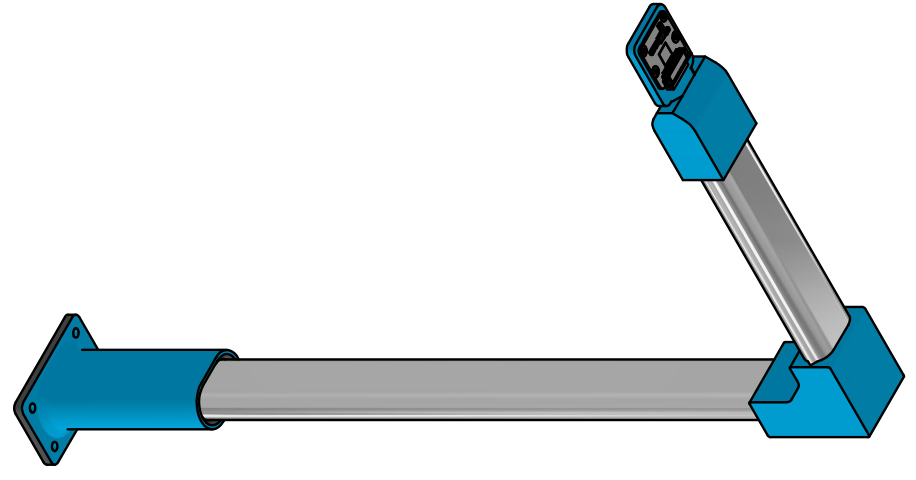
\includegraphics[width=0.55\textwidth]{06disenoConceptual/img/camara/soporteCamaraObsoleto.png}
    \caption{Primera iteración del soporte de cámara mostrando configuración tipo "L" con mástil vertical y viga horizontal en voladizo. Se observa el sistema de uniones por fricción entre tubo ovalado y piezas impresas en FDM.}
    \label{fig:soporteCamaraObsoleto}
\end{figure}

\begin{figure}[H]
    \centering
    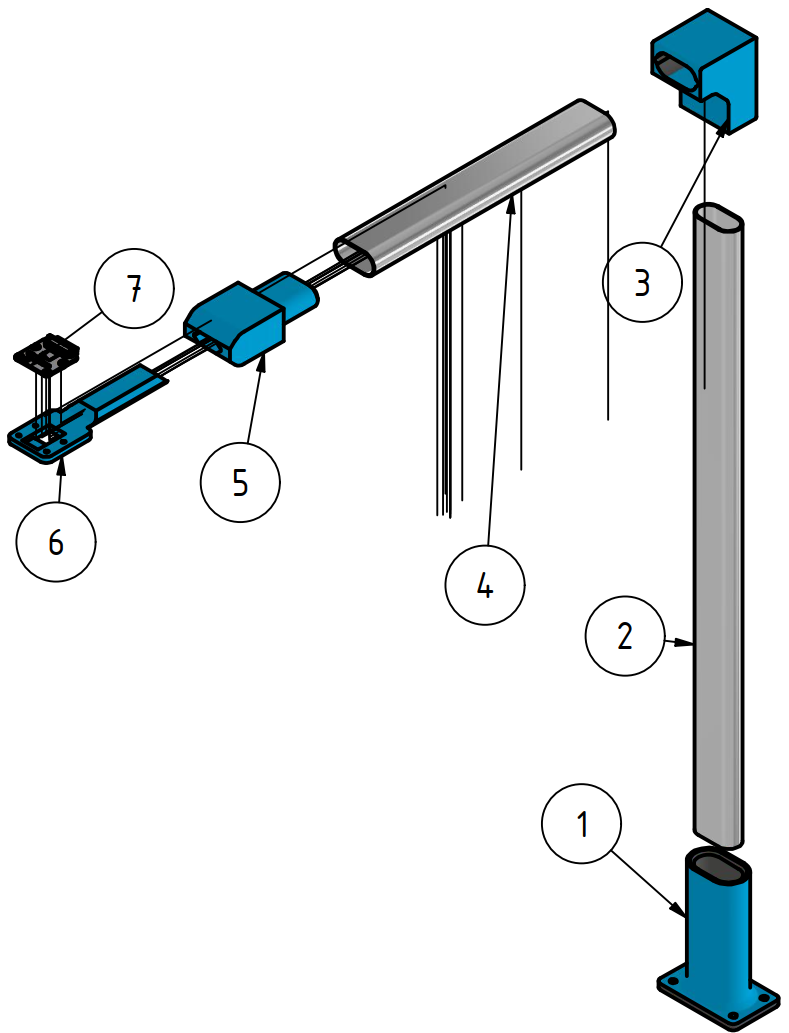
\includegraphics[width=0.6\textwidth]{06disenoConceptual/img/camara/ensambleSoporteCamaraViejo.png}
    \caption{Ensamble explosionado del diseño inicial. (1) Base de mástil con cavidad por fricción, (2) Mástil de tubo ovalado vertical, (3) Codo de 90° con doble cavidad de fricción, (4) Viga horizontal de tubo ovalado, (5) Acople viga-cámara por fricción, (6) Anclaje específico de cámara, (7) Cámara Logitech C270.}
    \label{fig:ensambleSoporteCamaraViejo}
\end{figure}

\begin{table}[H]
\centering
\caption{Componentes del diseño inicial de soporte de cámara}
\label{tab:soporte_camara_v1}
\small
\begin{tabular}{|c|l|c|l|l|}
\hline
\textbf{\#} & \textbf{Componente} & \textbf{Cant.} & \textbf{Fabricación} & \textbf{Material} \\
\hline
1 & Base de mástil & 1 & FDM & ABS/PETG \\
2 & Mástil & 1 & Comercial + corte & Aluminio \\
3 & Codo 90° & 1 & FDM & ABS/PETG \\
4 & Viga & 1 & Comercial + corte & Aluminio \\
5 & Acople viga-cámara & 1 & FDM & ABS/PETG \\
6 & Anclaje de cámara & 1 & FDM & ABS/PETG \\
7 & Cámara & 1 & Comercial & --- \\
\hline
\end{tabular}
\end{table}

\paragraph{Deficiencias Identificadas}

A pesar de la simplicidad conceptual, el diseño por fricción presentó deficiencias críticas durante pruebas de operación extendida:

\begin{itemize}
    \item \textbf{Desgaste de interfaces}: Las cavidades de fricción en piezas FDM (base de mástil, codo, acople de viga) experimentaban deformación plástica progresiva por ciclos de carga/descarga durante vibraciones del manipulador
    
    \item \textbf{Desarrollo de juego mecánico}: Tras 50-100 horas de operación, se observó holgura de 2-5 mm en las uniones, resultando en movimiento de la cámara y pérdida de calibración
    
    \item \textbf{Inestabilidad creciente}: El juego acumulado en múltiples interfaces producía amplificación de vibraciones, comprometiendo la calidad de captura de imágenes
    
    \item \textbf{Ausencia de ajustabilidad}: Una vez instalado, no existía mecanismo para compensar el desgaste sin reemplazar componentes completos
\end{itemize}

Estas deficiencias fundamentaron el desarrollo de una segunda iteración con sistema de fijación mecánica positiva.

\subsubsection{Segunda Iteración: Diseño con Fijación Roscada}

La segunda iteración abandona el concepto de fricción en favor de un sistema de fijación roscada que proporciona rigidez sostenida y ajustabilidad. El diseño conserva modularidad para permitir adaptación a diferentes cámaras.

\paragraph{Versatilidad de Cámaras}

Si bien la selección final fue la Logitech C270, el diseño modular permite intercambio del anclaje de cámara para acomodar sensores alternativos. La Figura \ref{fig:ensamblesCamaras} presenta dos configuraciones: una con cámara ORBBEC Astra y otra con Logitech C270, demostrando la capacidad de adaptación mediante reemplazo del subconjunto de anclaje superior.

\begin{figure}[H]
    \centering
    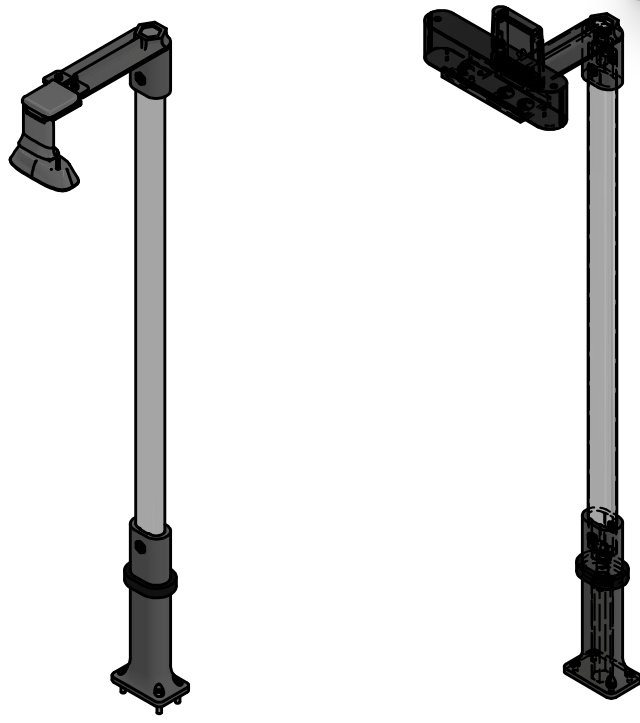
\includegraphics[width=0.7\textwidth]{06disenoConceptual/img/camara/ensamblesCamaras.png}
    \caption{Comparación de configuraciones del soporte con diferentes cámaras. Izquierda: Configuración con cámara ORBBEC Astra RGB-D. Derecha: Configuración con cámara Logitech C270 (seleccionada). Ambas utilizan el mismo mástil y base, intercambiando únicamente el subconjunto de anclaje superior.}
    \label{fig:ensamblesCamaras}
\end{figure}

Esta modularidad preserva inversión en componentes estructurales (mástil, base) si futuras iteraciones del kit requieren sensores con capacidades diferentes.

\paragraph{Determinación de Altura Operativa}

La altura del soporte se determinó empíricamente considerando el campo de visión de las cámaras evaluadas. Se realizaron pruebas de captura a diferentes alturas, identificando que para las cámaras Logitech C270 y ORBBEC Astra (ambas con FOV de aproximadamente 60° diagonal), la altura óptima se encuentra en el rango de 630-710 mm medidos desde la plataforma base hasta el centro del lente.

Esta altura proporciona:
\begin{itemize}
    \item Cobertura completa de la zona de recolección (Ø146 mm)
    \item Visualización de las cuatro zonas de depósito
    \item Margen perimetral de 50-80 mm para compensar desalineamientos
    \item Resolución de 3-4 píxeles/mm sobre objetos de 25 mm × 25 mm
\end{itemize}

\subsubsection{Arquitectura del Conjunto Completo}

El diseño final se estructura en tres subconjuntos principales interconectados mediante tornillería M10 y M4, como se observa en la Figura \ref{fig:ensambleSoporteCamara}.

\begin{figure}[H]
    \centering
    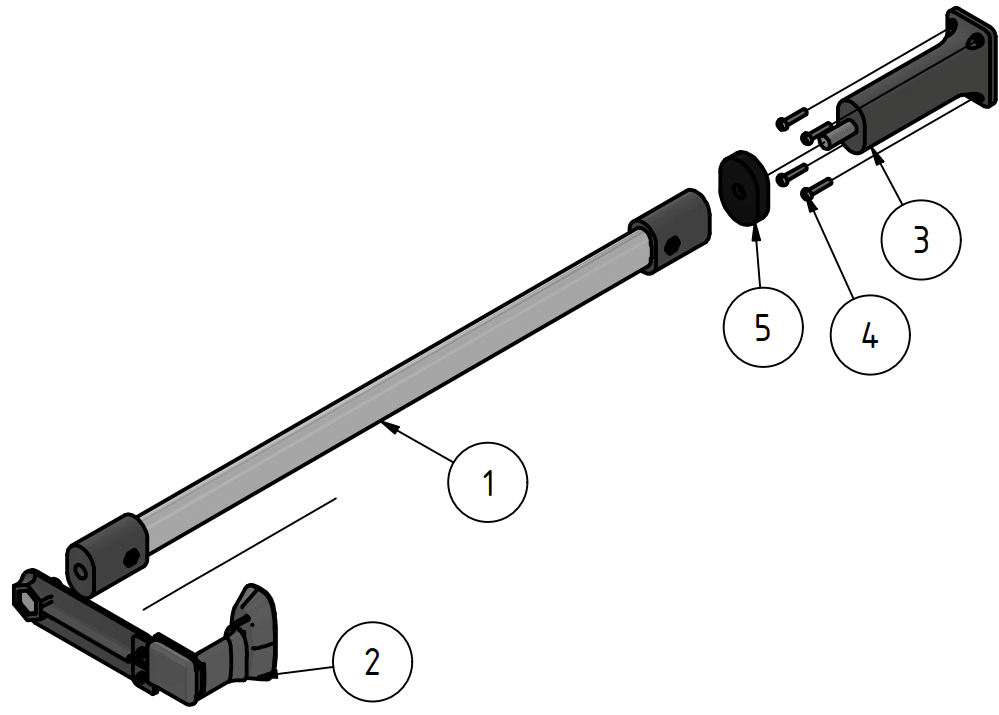
\includegraphics[width=0.8\textwidth]{06disenoConceptual/img/camara/ensambleSoporteCamara.png}
    \caption{Ensamble completo del soporte de cámara versión final. (1) Subconjunto de base de mástil anclado a plataforma, (2) Subconjunto de mástil con encajes roscados en extremos, (3) Subconjunto de soporte superior con viga en voladizo y anclaje de cámara, (4) Tornillos M4 × 20 mm para fijación de base a plataforma (4 unidades), (5) Arandela ovalada de TPU para amortiguación entre mástil y base.}
    \label{fig:ensambleSoporteCamara}
\end{figure}

\begin{table}[H]
\centering
\caption{Componentes principales del soporte de cámara versión final}
\label{tab:soporte_camara_v2}
\small
\begin{tabular}{|c|l|c|l|l|}
\hline
\textbf{\#} & \textbf{Componente} & \textbf{Cant.} & \textbf{Fabricación} & \textbf{Material} \\
\hline
1 & Subconjunto de mástil & 1 & --- & --- \\
2 & Subconjunto soporte superior & 1 & --- & --- \\
3 & Subconjunto base de mástil & 1 & --- & --- \\
4 & Tornillo M4 × 20 mm & 4 & Comercial & Acero \\
5 & Arandela ovalada & 1 & FDM & TPU \\
\hline
\end{tabular}
\end{table}

\paragraph{Función de la Arandela de TPU}

La arandela ovalada de TPU (poliuretano termoplástico) insertada entre el mástil y la base cumple funciones de amortiguación y distribución de carga:

\begin{itemize}
    \item \textbf{Amortiguación de vibraciones}: El TPU, con dureza Shore 95A típica, absorbe vibraciones de alta frecuencia transmitidas desde el manipulador a través de la plataforma
    \item \textbf{Compensación de irregularidades}: La flexibilidad del TPU compensa pequeñas irregularidades de fabricación en las interfaces
    \item \textbf{Distribución de presión}: Previene concentración de esfuerzos en el borde del encaje roscado del mástil
\end{itemize}

\subsubsection{Subconjunto de Mástil}

El mástil constituye el elemento estructural vertical del soporte. La Figura \ref{fig:ensambleMastil} presenta su configuración y la Figura \ref{fig:vistaInternaMastil} revela el mecanismo interno de bloqueo.

\begin{figure}[H]
    \centering
    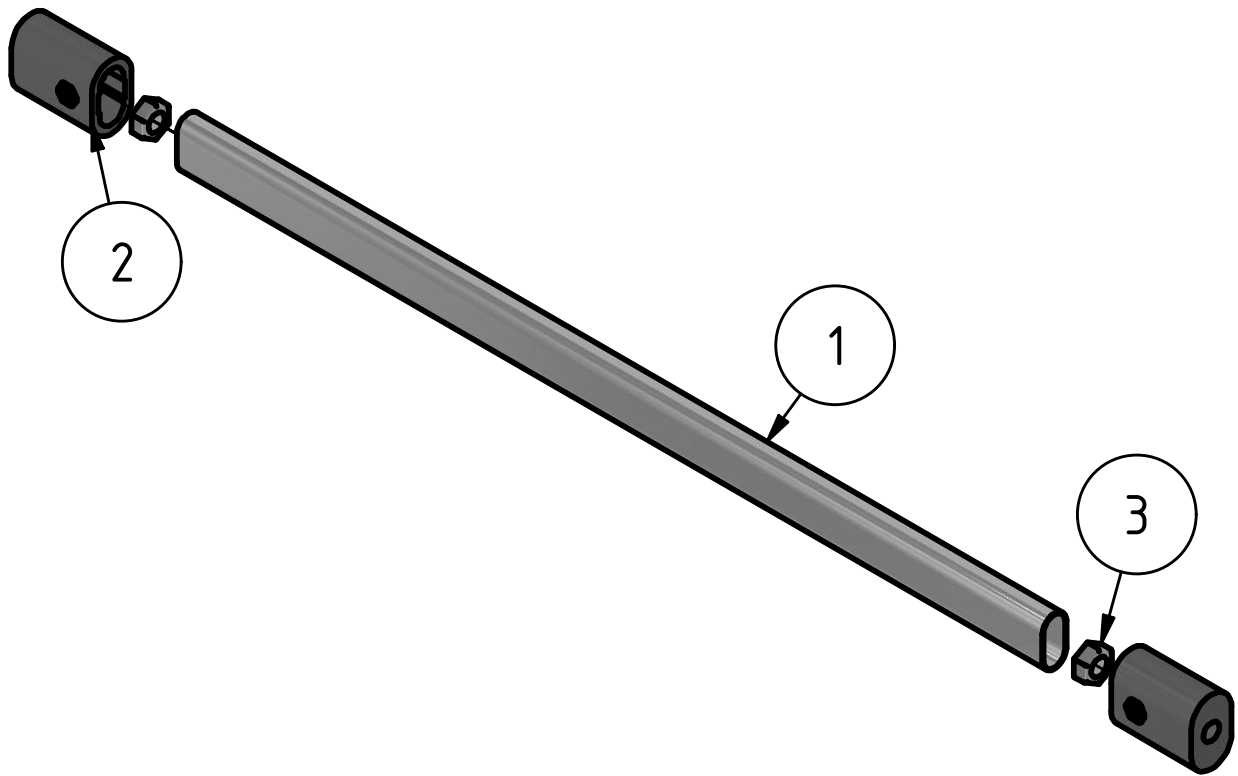
\includegraphics[width=0.6\textwidth]{06disenoConceptual/img/camara/ensambleMastil.png}
    \caption{Ensamble explosionado del subconjunto de mástil. (1) Tubo ovalado de aluminio de 540 mm de longitud, (2) Encajes de tubo a tuerca fabricados en PETG/ABS (2 unidades, superior e inferior), (3) Tuercas M10 alojadas en encajes (2 unidades).}
    \label{fig:ensambleMastil}
\end{figure}

\begin{figure}[H]
    \centering
    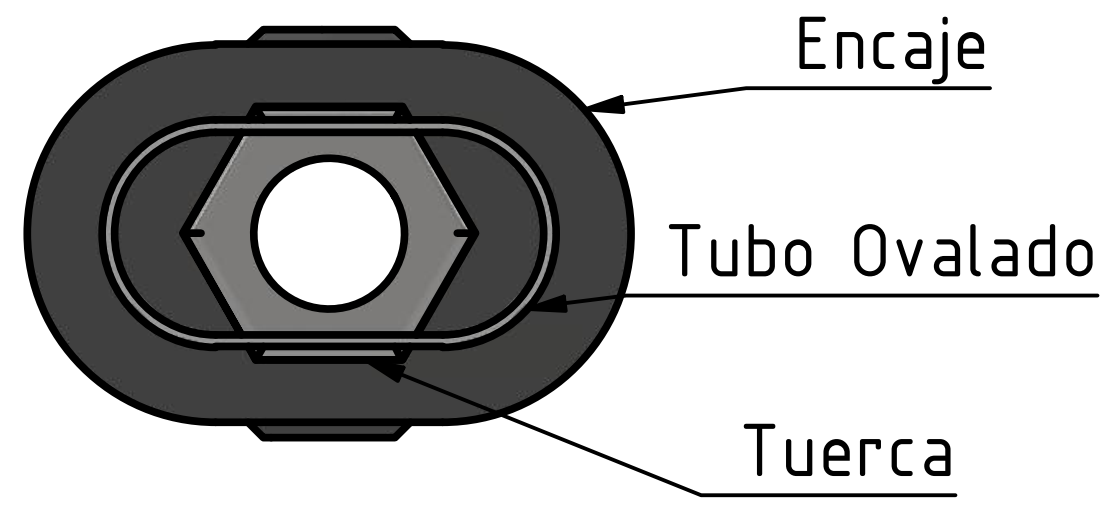
\includegraphics[width=0.5\textwidth]{06disenoConceptual/img/camara/vistaInternaMastil.png}
    \caption{Vista en corte del mecanismo de bloqueo del encaje. El tubo ovalado se inserta en el encaje mediante interferencia o impacto con martillo. Una vez insertado, el perfil ovalado del tubo bloquea la rotación de la tuerca M10 alojada en la cavidad hexagonal del encaje, permitiendo que tornillos externos se enrosquen en la tuerca sin que esta gire.}
    \label{fig:vistaInternaMastil}
\end{figure}

\begin{table}[H]
\centering
\caption{Componentes del subconjunto de mástil}
\label{tab:bom_mastil}
\small
\begin{tabular}{|c|l|c|l|l|}
\hline
\textbf{\#} & \textbf{Componente} & \textbf{Cant.} & \textbf{Fabricación} & \textbf{Material} \\
\hline
1 & Tubo ovalado 540 mm & 1 & Comercial + corte & Aluminio \\
2 & Encaje tubo-tuerca & 2 & FDM & ABS/PETG \\
3 & Tuerca M10 & 2 & Comercial & Acero \\
\hline
\end{tabular}
\end{table}

\paragraph{Restricción Dimensional del Mástil}

La longitud del tubo ovalado (540 mm) se determinó considerando la restricción crítica del contenedor. Durante almacenamiento, el mástil se posiciona diagonalmente dentro del contenedor plástico. Mediante análisis geométrico de la diagonal interna máxima del contenedor (566 mm × 366 mm × altura interna), se estableció que 540 mm es la longitud máxima que permite almacenamiento seguro con margen de 20-30 mm.

Incluyendo los encajes en ambos extremos (18 mm cada uno), la longitud total del subconjunto de mástil es de 576 mm, como se observa en la Figura \ref{fig:largosSoporteCamara}.

\begin{figure}[H]
    \centering
    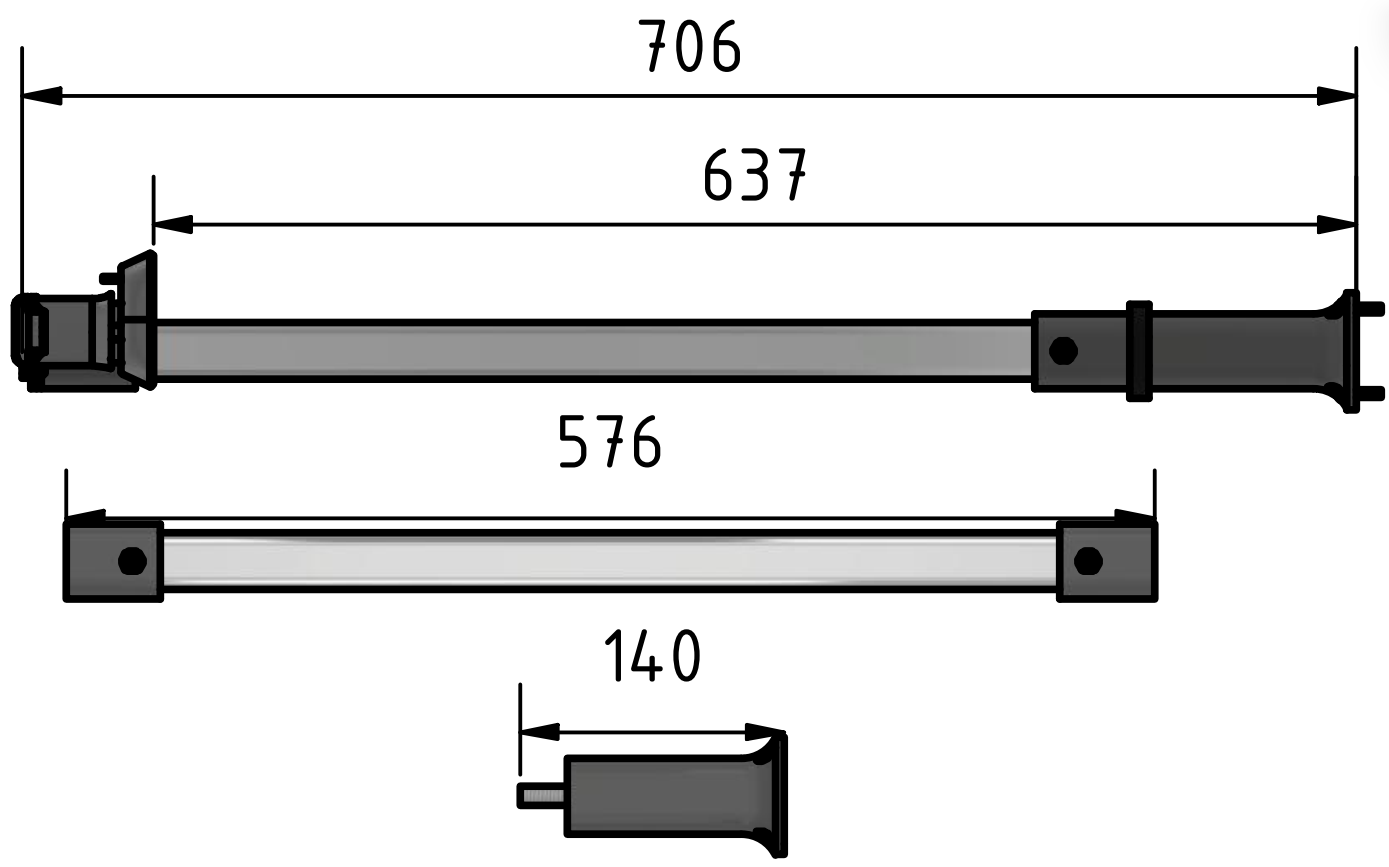
\includegraphics[width=0.85\textwidth]{06disenoConceptual/img/camara/largosSoporteCamara.png}
    \caption{Dimensiones principales de los subconjuntos del soporte de cámara. Superior: Subconjunto completo con longitud total de 706 mm desde base hasta extremo del anclaje de cámara, alcance horizontal de 637 mm desde eje del mástil. Centro: Subconjunto de mástil con longitud total de 576 mm (540 mm de tubo + 2 × 18 mm de encajes). Inferior: Subconjunto de base con altura de 140 mm (altura máxima permitida por contenedor).}
    \label{fig:largosSoporteCamara}
\end{figure}

\paragraph{Mecanismo de Bloqueo Anti-Rotación}

El diseño del encaje aprovecha la geometría ovalada del tubo para crear un sistema de bloqueo automático:

\begin{enumerate}
    \item El encaje se instala en el extremo del tubo mediante interferencia (ajuste apretado) o impacto controlado con martillo de goma
    \item La cavidad interior del encaje tiene geometría ovalada que coincide exactamente con el perfil del tubo
    \item La tuerca M10 se aloja en una cavidad hexagonal dentro del encaje
    \item Cuando el tubo está insertado, su geometría ovalada bloquea completamente la rotación de la tuerca
    \item Tornillos M10 externos pueden enroscarse en la tuerca sin que esta gire, creando unión estructural rígida
\end{enumerate}

Este mecanismo elimina la necesidad de sostener la tuerca con herramientas durante ensamblaje, simplificando el montaje del sistema completo.

\paragraph{Selección de Material PETG/ABS para Encajes}

Los encajes se fabrican en PETG o ABS en lugar de PLA por consideraciones de propiedades mecánicas:

\begin{itemize}
    \item \textbf{Resistencia a impacto}: PETG/ABS absorben energía de impacto durante instalación sin fracturarse (instalación con martillo)
    \item \textbf{Resistencia a fluencia}: Mayor resistencia a deformación plástica bajo carga sostenida que PLA
    \item \textbf{Tenacidad}: Módulo de elasticidad ligeramente inferior al PLA permite pequeñas deformaciones elásticas sin fractura
    \item \textbf{Estabilidad dimensional}: Menor susceptibilidad a cambios dimensionales por absorción de humedad
\end{itemize}

\subsubsection{Subconjunto de Base de Mástil}

La base del mástil proporciona la interfaz entre el tubo vertical y la plataforma del kit. La Figura \ref{fig:ensambleBaseCamara} presenta su configuración interna.

\begin{figure}[H]
    \centering
    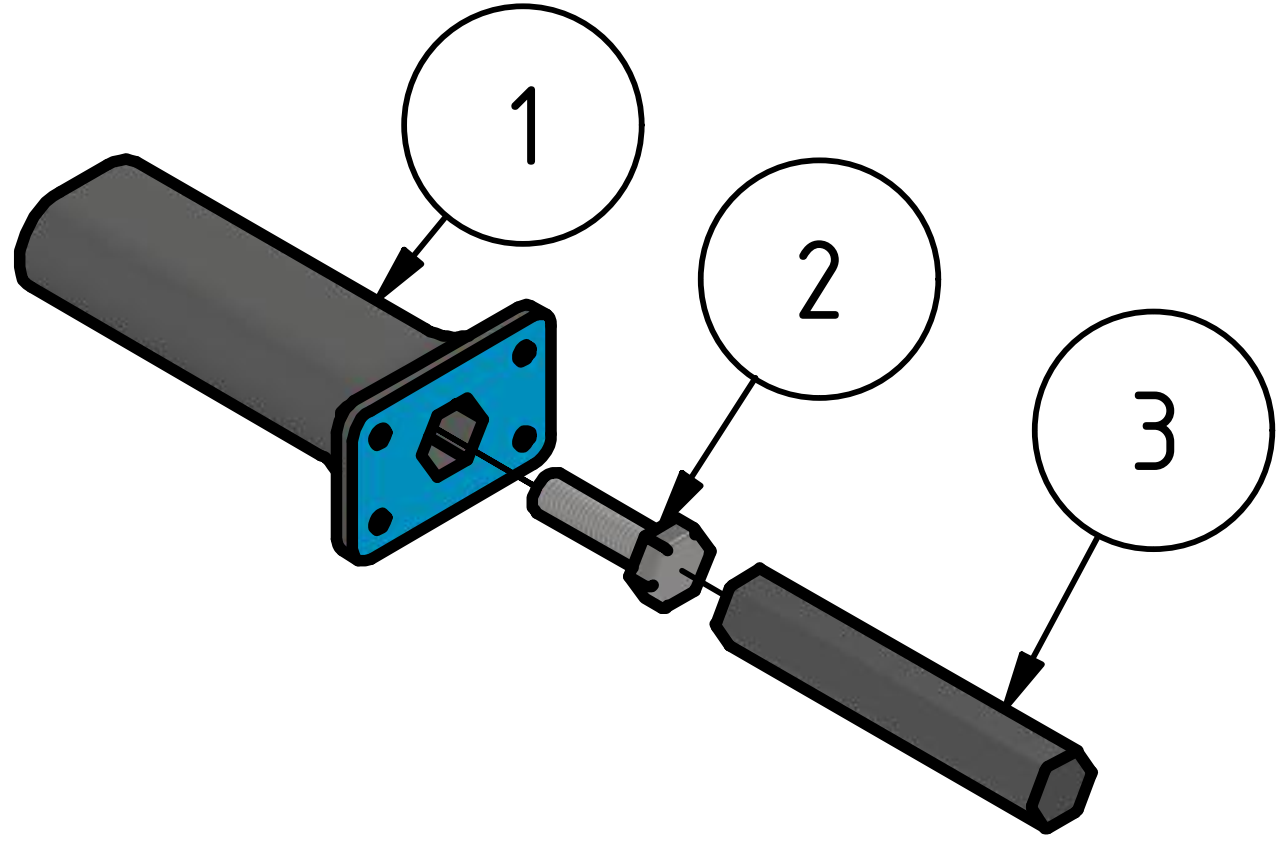
\includegraphics[width=0.55\textwidth]{06disenoConceptual/img/camara/ensambleBaseCamara.png}
    \caption{Ensamble del subconjunto de base de mástil. (1) Tubo ovalado del mástil insertándose en cavidad superior, (2) Tornillo M10 × 35 mm actuando como perno de conexión, (3) Barra hexagonal de refuerzo estructural unida permanentemente con silicona caliente al tornillo y a la base.}
    \label{fig:ensambleBaseCamara}
\end{figure}

\begin{table}[H]
\centering
\caption{Componentes del subconjunto de base de mástil}
\label{tab:bom_base_mastil}
\small
\begin{tabular}{|c|l|c|l|l|}
\hline
\textbf{\#} & \textbf{Componente} & \textbf{Cant.} & \textbf{Fabricación} & \textbf{Material} \\
\hline
1 & Base de mástil & 1 & FDM & ABS/PETG \\
2 & Tornillo M10 × 35 mm & 1 & Comercial & Acero \\
3 & Barra hexagonal de refuerzo & 1 & FDM & ABS/PETG \\
\hline
\end{tabular}
\end{table}

\paragraph{Arquitectura Interna de Refuerzo}

La base incorpora un sistema de refuerzo estructural mediante barra hexagonal interna:

\begin{itemize}
    \item \textbf{Componente}: Barra hexagonal maciza impresa con eje longitudinal paralelo al plano de la cama de impresión
    \item \textbf{Función mecánica}: Resiste cargas de flexión y tensión transmitidas desde el mástil
    \item \textbf{Ventaja de orientación de impresión}: Las capas de impresión quedan orientadas perpendiculares a la dirección de carga principal, aprovechando la mayor resistencia del filamento en dirección paralela a las capas
    \item \textbf{Ensamblaje}: Se une permanentemente al tornillo M10 y a las paredes internas de la base mediante silicona caliente durante fabricación
\end{itemize}

\paragraph{Restricción de Altura por Contenedor}

La altura de la base (140 mm) está limitada por la altura interna del contenedor plástico. Si la base excediera esta dimensión, el contenedor no podría cerrarse correctamente. La Figura \ref{fig:vistaInternaKitBaseMastil} ilustra esta restricción crítica de diseño.

\begin{figure}[H]
    \centering
    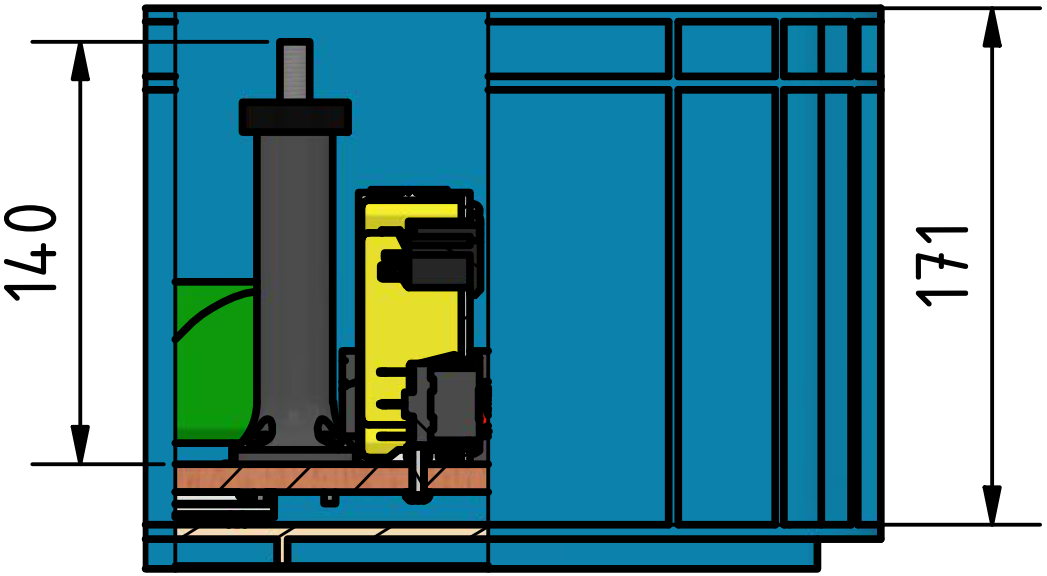
\includegraphics[width=0.75\textwidth]{06disenoConceptual/img/camara/vistaInternaKitBaseMastil.png}
    \caption{Vista en corte del interior del contenedor con base de mástil instalada. Altura interna del contenedor: 171 mm. Altura de la base: 140 mm. La base (verde) no excede la altura interna, permitiendo cierre correcto de la tapa. Se observa la arandela de TPU (naranja) entre base y plataforma.}
    \label{fig:vistaInternaKitBaseMastil}
\end{figure}

\paragraph{Consideraciones de Orientación de Impresión}

La base del mástil se imprime con su eje longitudinal perpendicular a la cama de impresión (vertical). Esta orientación:

\begin{itemize}
    \item \textbf{Ventaja geométrica}: Minimiza soportes y facilita extracción de la pieza
    \item \textbf{Desventaja mecánica}: Las capas quedan paralelas a la dirección de carga de tensión, reduciendo resistencia en aproximadamente 30-40\% respecto a orientación horizontal
    \item \textbf{Compensación}: La barra hexagonal interna, impresa horizontalmente, compensa esta debilidad proporcionando el 60-70\% de la resistencia estructural del conjunto
\end{itemize}

\subsubsection{Subconjunto de Soporte Superior}

El soporte superior constituye el elemento en voladizo que posiciona la cámara sobre el centro de la zona de trabajo. La Figura \ref{fig:soporteSuperiorC270} presenta su configuración modular.

\begin{figure}[H]
    \centering
    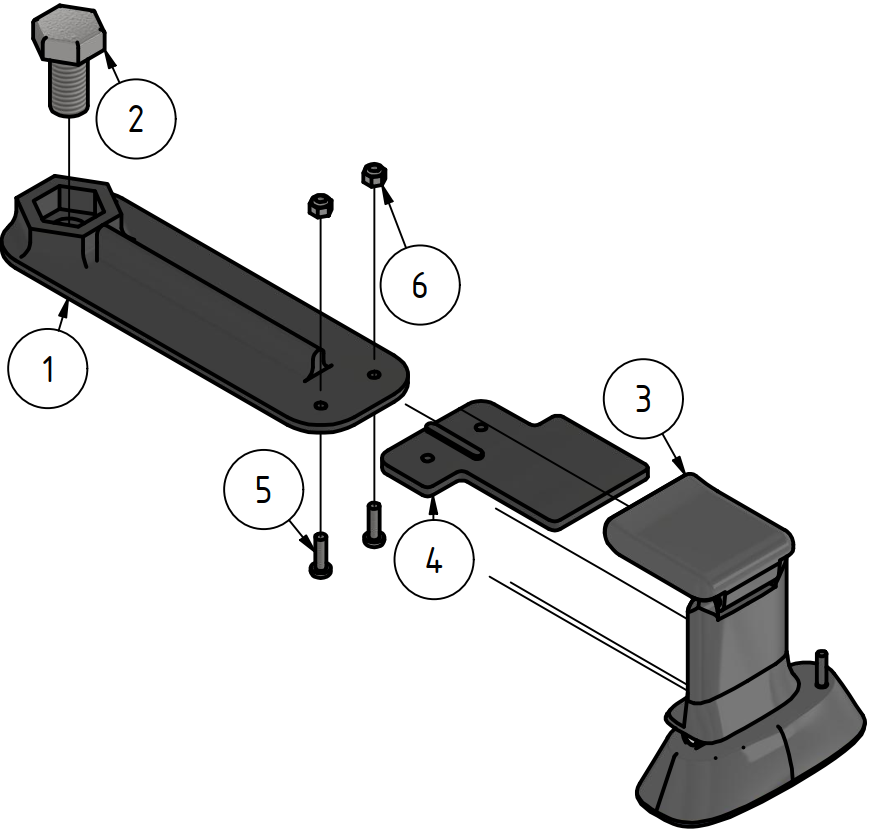
\includegraphics[width=0.75\textwidth]{06disenoConceptual/img/camara/soporteSuperiorC270.png}
    \caption{Ensamble del subconjunto de soporte superior para cámara Logitech C270. (1) Viga de soporte fabricada en PETG/ABS, (2) Tornillo M10 × 20 mm unido permanentemente a la viga con silicona, que se enrosca en tuerca del extremo superior del mástil, (3) Cámara Logitech C270, (4) Anclaje modular específico de cámara, (5) Tornillos M3 × 10 mm (2 unidades), (6) Tuercas de seguridad M3 (2 unidades).}
    \label{fig:soporteSuperiorC270}
\end{figure}

\begin{table}[H]
\centering
\caption{Componentes del subconjunto de soporte superior}
\label{tab:bom_soporte_superior}
\small
\begin{tabular}{|c|l|c|l|l|}
\hline
\textbf{\#} & \textbf{Componente} & \textbf{Cant.} & \textbf{Fabricación} & \textbf{Material} \\
\hline
1 & Viga de soporte de cámara & 1 & FDM & ABS/PETG \\
2 & Tornillo M10 × 20 mm & 1 & Comercial & Acero \\
3 & Cámara Logitech C270 & 1 & Comercial & --- \\
4 & Anclaje de cámara a viga & 1 & FDM & ABS/PETG \\
5 & Tornillo M3 × 10 mm & 2 & Comercial & Acero \\
6 & Tuerca de seguridad M3 & 2 & Comercial & Acero \\
\hline
\end{tabular}
\end{table}

\paragraph{Conexión Viga-Mástil}

La viga se une al mástil mediante tornillo M10 × 20 mm que se enrosca en la tuerca cautiva del encaje superior del mástil. El tornillo se fija permanentemente a la viga mediante silicona caliente aplicada en una cavidad interna, garantizando que:

\begin{itemize}
    \item El tornillo no se afloje por vibraciones durante operación
    \item La unión viga-mástil pueda ajustarse o removerse desenroscando el tornillo sin que este se separe de la viga
    \item La orientación angular de la viga respecto al mástil pueda ajustarse durante instalación inicial
\end{itemize}

\paragraph{Modularidad del Anclaje de Cámara}

El anclaje de cámara se diseña específicamente para cada modelo de cámara contemplado. Para la Logitech C270, el anclaje:

\begin{itemize}
    \item Abraza el cuerpo cilíndrico de la cámara con geometría complementaria
    \item Se fija a la viga mediante dos tornillos M3 × 10 mm con tuercas de seguridad
    \item Permite ajuste de inclinación (±10°) antes de apriete final
    \item Posiciona el lente de la cámara alineado con el centro de la zona de recolección
\end{itemize}

Para cámaras alternativas (ORBBEC Astra, Intel RealSense), solo requiere reemplazo del anclaje específico, reutilizando viga, mástil y base.

\paragraph{Alineación Óptica}

El diseño del anclaje garantiza que el centro óptico del lente de la cámara esté alineado con el eje vertical que pasa por el centro de la zona de recolección (Ø146 mm, blanca). La Figura \ref{fig:vistaSuperiorCamaraKit} demuestra esta alineación en vista superior.

\begin{figure}[H]
    \centering
    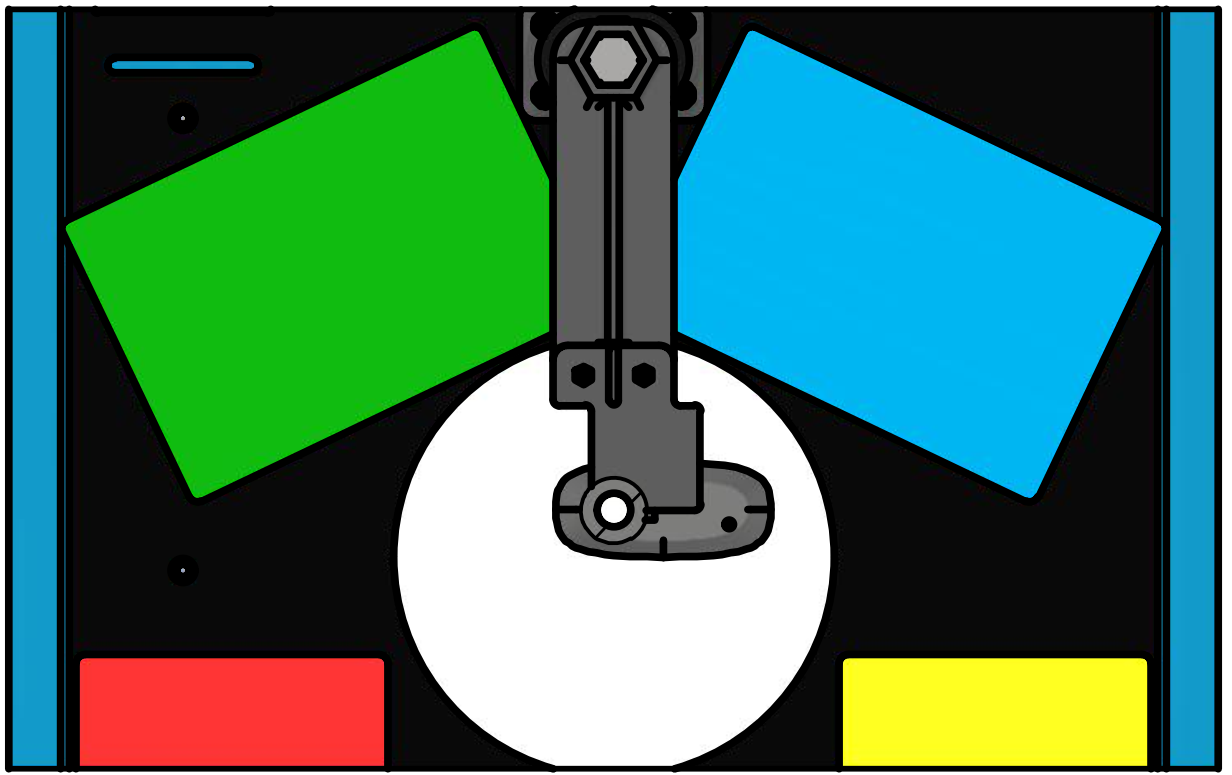
\includegraphics[width=0.8\textwidth]{06disenoConceptual/img/camara/vistaSuperiorCamaraKit.png}
    \caption{Vista superior del kit mostrando alineación del eje óptico de la cámara. El centro del lente (indicado por proyección vertical) coincide con el centro geométrico de la zona de recolección (blanca, Ø146 mm). Esta alineación minimiza distorsión perspectiva en los bordes de la zona de trabajo y simplifica la calibración del sistema de visión.}
    \label{fig:vistaSuperiorCamaraKit}
\end{figure}

Esta alineación centrada proporciona:
\begin{itemize}
    \item Distorsión perspectiva simétrica respecto al centro de la imagen
    \item Simplificación de transformaciones pixel-a-mundo (matriz homográfica con punto principal centrado)
    \item Cobertura equidistante de zonas de depósito desde el centro óptico
    \item Reducción de oclusiones en bordes de la zona de recolección
\end{itemize}

\subsection{Conclusión del Diseño del Soporte}

El diseño final del soporte de cámara representa una evolución significativa respecto a la iteración inicial, incorporando lecciones aprendidas sobre desgaste de interfaces y estabilidad dimensional. El sistema de fijación roscada M10 proporciona rigidez sostenida, la arquitectura modular permite adaptación a diferentes sensores, y las restricciones dimensionales del contenedor se satisfacen mediante optimización de alturas y longitudes. El resultado es un soporte robusto, ajustable y versátil que garantiza posicionamiento estable del sensor visual durante operación extendida del kit educativo.
\subsection{Diseño de Objetos de Clasificación}

Los objetos de clasificación constituyen los elementos manipulables del kit que los estudiantes programarán al robot para detectar, recoger y depositar en las zonas correspondientes. Su diseño debe equilibrar facilidad de detección por visión por computador, compatibilidad con el sistema de succión por vacío y robustez operativa.

\subsubsection{Requerimientos de Diseño}

Los objetos de clasificación deben cumplir los siguientes criterios:

\paragraph{Requerimientos Geométricos}

\begin{itemize}
    \item Dimensión característica base: 25 mm × 25 mm (compatible con ventosa Ø15 mm con holgura de 5 mm)
    \item Altura uniforme: 25 mm para todos los objetos
    \item Geometrías distinguibles mediante algoritmos de detección de formas
    \item Superficie superior plana y lisa para contacto óptimo con ventosa
    \item Estabilidad cuando se colocan sobre superficie plana
\end{itemize}

\paragraph{Requerimientos de Percepción Visual}

\begin{itemize}
    \item Color uniforme y distinguible del entorno
    \item Contraste elevado respecto a fondo blanco (zona de recolección) y negro (plataforma base)
    \item Diferenciación respecto a colores de zonas de depósito (rojo, verde, azul, amarillo)
    \item Superficie mate para minimizar reflejos bajo iluminación artificial
\end{itemize}

\subsubsection{Geometrías Seleccionadas}

Se diseñaron cuatro geometrías básicas distinguibles tanto por forma como por número de vértices o curvatura. La Figura \ref{fig:objetosRecoleccion} presenta las dimensiones de cada tipo.

\begin{figure}[H]
    \centering
    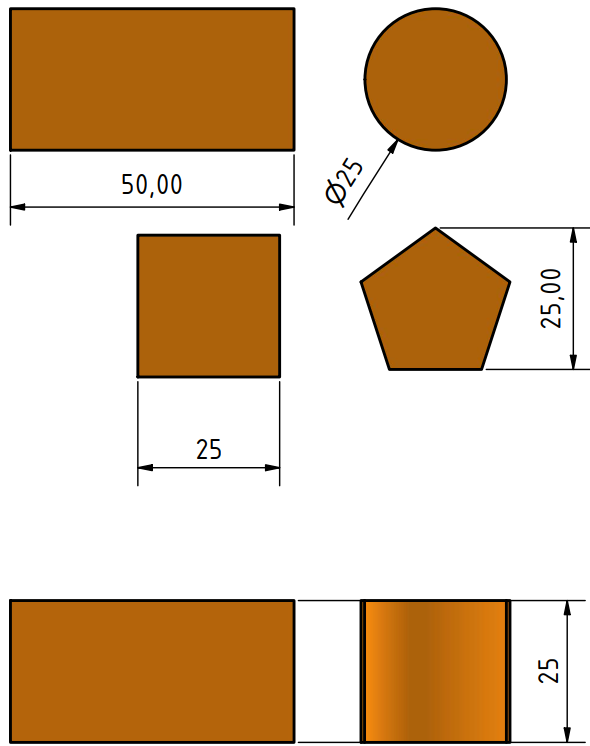
\includegraphics[width=0.4\textwidth]{06disenoConceptual/img/zonaRecoleccion/objetosRecoleccion.png}
    \caption{Geometrías de objetos de clasificación con dimensiones principales. Superior izquierda: Rectángulo 50 mm × 25 mm. Superior centro: Cuadrado 25 mm × 25 mm. Superior derecha: Círculo Ø25 mm. Centro derecha: Pentágono regular inscrito en círculo de 25 mm de diámetro. Inferior: Vista lateral mostrando altura uniforme de 25 mm para todos los objetos. Color: Naranja uniforme.}
    \label{fig:objetosRecoleccion}
\end{figure}

\paragraph{Cuadrado (25 mm × 25 mm)}

\begin{itemize}
    \item Dimensiones: 25 mm × 25 mm × 25 mm (cubo perfecto)
    \item Características: 4 vértices, 4 lados iguales, relación aspecto 1:1
    \item Ventaja didáctica: Forma más simple, facilita validación inicial de algoritmos
\end{itemize}

\paragraph{Rectángulo (50 mm × 25 mm)}

\begin{itemize}
    \item Dimensiones: 50 mm × 25 mm × 25 mm
    \item Características: 4 vértices, relación aspecto 2:1
    \item Ventaja didáctica: Introduce concepto de orientación (eje mayor/menor)
\end{itemize}

\paragraph{Círculo (Ø25 mm)}

\begin{itemize}
    \item Dimensiones: Ø25 mm × 25 mm de altura
    \item Características: Ausencia de vértices, geometría circular perfecta
    \item Ventaja didáctica: Invarianza a rotación, prueba de algoritmos de circularidad
\end{itemize}

\paragraph{Pentágono Regular (Ø25 mm circunscrito)}

\begin{itemize}
    \item Dimensiones: Pentágono regular inscrito en círculo Ø25 mm, altura 25 mm
    \item Características: 5 vértices, ángulos internos de 108°
    \item Ventaja didáctica: Forma más compleja, requiere algoritmos robustos de detección de vértices
\end{itemize}

\subsubsection{Selección de Color}

Se seleccionó el color naranja como color uniforme para todos los objetos de clasificación, fundamentado en criterios de diferenciación cromática.

\paragraph{Contraste con Elementos del Sistema}

El naranja proporciona máxima diferenciación respecto a todos los elementos cromáticos del kit:

\begin{itemize}
    \item \textbf{Plataforma base}: Negro, contraste por luminosidad muy elevado
    \item \textbf{Zona de recolección}: Blanca, contraste por saturación
    \item \textbf{Zonas de depósito}: Rojo, verde, azul y amarillo, diferenciable por tonalidad
\end{itemize}

Esta diferenciación cromática facilita la segmentación de objetos mediante algoritmos de procesamiento de imágenes, permitiendo detección robusta bajo condiciones de iluminación artificial típicas de laboratorio.

\subsubsection{Material de Fabricación}

Los objetos se fabrican mediante FDM utilizando TPU (poliuretano termoplástico) en color naranja. La selección de TPU se fundamenta en su flexibilidad, que proporciona ventajas significativas:

\begin{itemize}
    \item \textbf{Mayor adherencia a la ventosa}: La superficie flexible del TPU se adapta mejor a la geometría de la ventosa de silicona, mejorando el sellado y la fuerza de succión
    \item \textbf{Resistencia a impactos}: El material flexible absorbe energía durante manipulación, reduciendo riesgo de fractura por caídas o colisiones
    \item \textbf{Amortiguación}: La flexibilidad reduce el impacto que el  objeto tiene en la pinza del robot.
\end{itemize}

\subsection{Diseño de Multitoma Personalizada}

El kit requiere un sistema de distribución de energía eléctrica que alimente simultáneamente múltiples componentes con diferentes requerimientos de potencia. La ausencia de soluciones comerciales que satisfagan las necesidades específicas del proyecto motivó el diseño de una multitoma personalizada integrada a la plataforma base.

\subsubsection{Justificación del Diseño Personalizado}

La necesidad de una multitoma personalizada se fundamenta en las siguientes consideraciones operativas y técnicas:

\begin{itemize}
    \item \textbf{Limitación de tomas disponibles}: El laboratorio (Sala CAM) cuenta con número limitado de tomas de corriente por estación de trabajo, requiriendo centralización de alimentación
    
    \item \textbf{Fuentes existentes de dimensiones variables}: Los robots PhantomX Pincher poseen fuentes de alimentación de diferentes generaciones con geometrías no estándar
    
    \item \textbf{Reutilización de componentes}: Se busca aprovechar fuentes de alimentación existentes en el inventario del laboratorio
    
    \item \textbf{Nuevos requerimientos de alimentación}: La Raspberry Pi 5 requiere fuente USB-C Power Delivery no contemplada en kits originales
    
    \item \textbf{Flexibilidad operativa}: Se requiere conexión simultánea de robot, Raspberry Pi, bomba de vacío y equipo auxiliar (PC para desarrollo)
    
    \item \textbf{Control individual de energización}: Se necesitan interruptores independientes para cada subsistema como medida de seguridad y apagado de emergencia
\end{itemize}

Multitomas comerciales estándar no permiten:
\begin{itemize}
    \item Espaciamiento variable entre tomas para acomodar fuentes de geometrías irregulares
    \item Control individual mediante switches iluminados con identificación específica
    \item Integración mecánica con la plataforma base del kit
    \item Fusible de protección accesible para reemplazo
\end{itemize}

\subsubsection{Análisis de Requerimientos Eléctricos}

\paragraph{Consumo de Corriente por Subsistema}

El dimensionamiento eléctrico de la multitoma se basó en el consumo máximo de cada componente del kit:

\begin{itemize}
    \item \textbf{Raspberry Pi 5}: Fuente USB-C 5V/3A (consumo real máximo ~1.5 A @ 5V)
    \item \textbf{Robot PhantomX Pincher}: Fuente 12V/3A (consumo máximo con 5 servomotores bajo carga)
    \item \textbf{Bomba de vacío 370A}: Consumo directo 12V/1A máximo (0.42 A nominal)
    \item \textbf{Equipo auxiliar}: PC o monitor para desarrollo, estimado 3A máximo @ 120V
\end{itemize}

\paragraph{Corriente Total de Diseño}

Considerando operación simultánea de todos los subsistemas:

\begin{equation}
I_{total} = I_{RPi} + I_{robot} + I_{bomba} + I_{aux} = 1.5 + 3.0 + 1.0 + 3.0 = 8.5 \text{ A}
\end{equation}

Se establece corriente de diseño de 9.5 A con margen de seguridad del 12\%, valor confortablemente inferior al límite de 15 A de los componentes comerciales seleccionados.

\subsubsection{Cumplimiento Normativo de Cableado}

El cableado interno de la multitoma se diseñó siguiendo el Reglamento Técnico de Instalaciones Eléctricas (RETIE) vigente en Colombia \cite{RETIE2013}:

\begin{itemize}
    \item \textbf{Conductor de fase}: Cable rojo, calibre 14 AWG
    \item \textbf{Conductor neutro}: Cable blanco, calibre 14 AWG
    \item \textbf{Conductor de tierra}: Cable verde, calibre 14 AWG
\end{itemize}

El calibre 14 AWG (2.08 mm², capacidad 15 A) proporciona margen del 58\% respecto a corriente de diseño (9.5 A), garantizando operación sin calentamiento excesivo.

\subsubsection{Sistemas de Seguridad Eléctrica}

La multitoma incorpora múltiples niveles de protección:

\paragraph{Protección por Fusible}

\begin{itemize}
    \item Fusible tipo cartucho 15 A, 125 V AC
    \item Ubicado en conector de entrada AC-01
    \item Protección contra sobrecorriente por cortocircuito o falla de equipo
    \item Accesible para reemplazo sin desmontar carcasa
\end{itemize}

\paragraph{Control Individual por Subsistema}

Se implementaron tres switches balancín independientes:

\begin{enumerate}
    \item \textbf{Switch 1}: Robot PhantomX Pincher + Bomba de vacío (circuito común 12V)
    \item \textbf{Switch 2}: Raspberry Pi 5 (alimentación independiente 5V)
    \item \textbf{Switch 3}: Toma auxiliar para PC o equipo de desarrollo
\end{enumerate}

Cada switch cuenta con indicador luminoso (piloto LED integrado) que señaliza estado energizado/desenergizado.

\paragraph{Interruptor Maestro}

El conector de entrada AC-01 incorpora switch balancín maestro que energiza o desenergiza simultáneamente todos los circuitos derivados, funcionando como:
\begin{itemize}
    \item Apagado de emergencia de todo el sistema
    \item Desconexión completa durante almacenamiento o transporte
    \item Protección contra arranque inadvertido
\end{itemize}

\subsubsection{Dimensionamiento Geométrico}

El espaciamiento entre tomas se determinó mediante modelado 3D de las fuentes de alimentación existentes en el inventario del laboratorio. La Figura \ref{fig:fuentesVarias} presenta las cinco fuentes consideradas.

\begin{figure}[H]
    \centering
    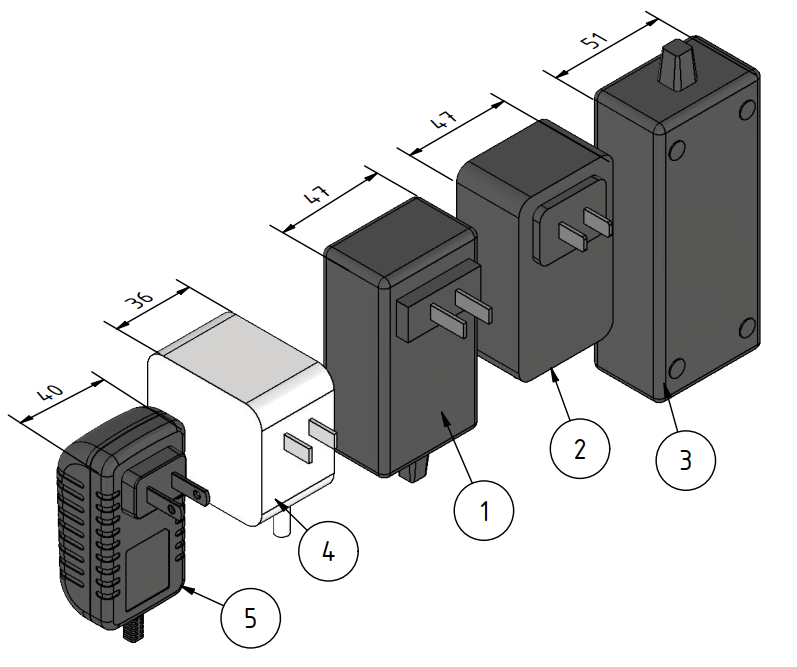
\includegraphics[width=0.7\textwidth]{06disenoConceptual/img/multitoma/fuentesVarias.png}
    \caption{Fuentes de alimentación modeladas para definir espaciamiento de tomas. (1) Fuente 12V/4A, largo 47 mm. (2) Fuente 12V/3A, largo 47 mm. (3) Fuente 12V/3A, largo 51 mm (geometría más grande). (4) Fuente 5V/5A USB-C para Raspberry Pi, largo 36 mm. (5) Fuente 12V/1A para bomba de vacío, largo 40 mm.}
    \label{fig:fuentesVarias}
\end{figure}

\begin{table}[H]
\centering
\caption{Fuentes de alimentación consideradas en el diseño}
\label{tab:fuentes_poder}
\small
\begin{tabular}{|c|l|c|}
\hline
\textbf{\#} & \textbf{Especificación} & \textbf{Largo (mm)} \\
\hline
1 & Fuente 12V/4A & 47 \\
2 & Fuente 12V/3A & 47 \\
3 & Fuente 12V/3A & 51 \\
4 & Fuente 5V/5A (USB-C) & 36 \\
5 & Fuente 12V/1A & 40 \\
\hline
\end{tabular}
\end{table}

\paragraph{Criterio de Espaciamiento}

Se estableció espaciamiento centro-a-centro de 26 mm para tres tomas principales, resultando en ocupación de 52 mm por toma (26 mm + 26 mm). Este espaciamiento acomoda la fuente más grande (51 mm) con holgura de 1 mm.

Para la toma destinada a la bomba de vacío (fuente de 40 mm), se redujo el espaciamiento a 22.5 mm centro-a-centro, optimizando el largo total de la multitoma.

\paragraph{Sistema de Identificación}

La carcasa incorpora marquillas grabadas en relieve que identifican la función de cada switch y toma:
\begin{itemize}
    \item "ROBOT" - Alimentación del manipulador PhantomX Pincher
    \item "VENTOSA" - Alimentación de bomba de vacío 370A
    \item "PI" - Alimentación de Raspberry Pi 5
    \item "PC" - Toma auxiliar de uso general
\end{itemize}

La Figura \ref{fig:vistasMultitoma} presenta vistas ortogonales de la multitoma con fuentes instaladas y sistema de identificación.

\begin{figure}[H]
    \centering
    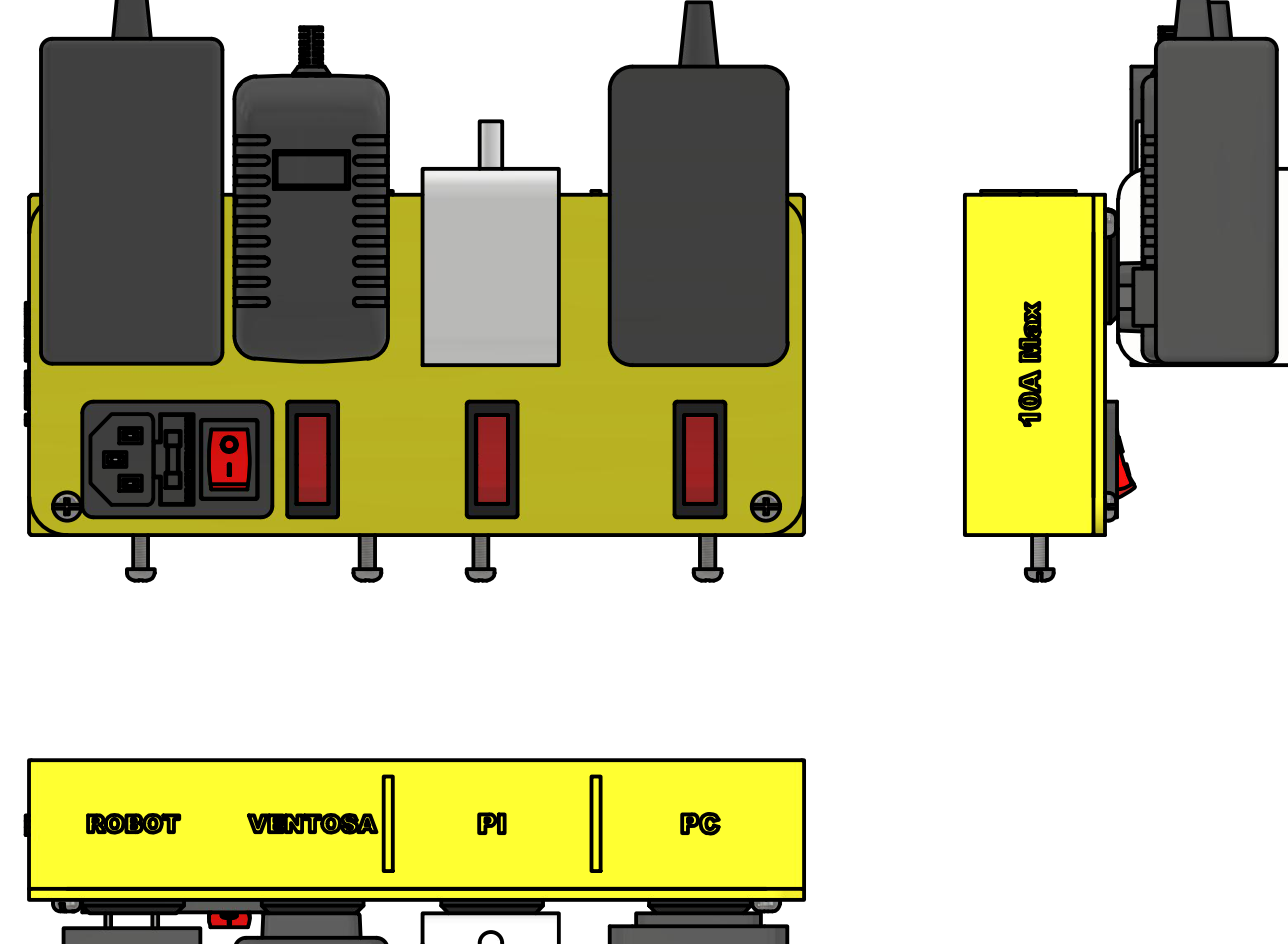
\includegraphics[width=0.95\textwidth]{06disenoConceptual/img/multitoma/vistasMultitoma.png}
    \caption{Vistas ortogonales de la multitoma con fuentes de poder instaladas. Vista frontal superior: Se observan cinco fuentes conectadas con espaciamiento optimizado. Los switches balancín (rojos) controlan energización individual. Vista lateral derecha: Perfil compacto con marquilla de capacidad máxima "10A Max". Vista inferior: Se muestran marquillas de identificación "ROBOT", "VENTOSA", "PI", "PC" que indican función de cada circuito. El conector AC-01 (izquierda) cuenta con switch maestro y fusible integrado.}
    \label{fig:vistasMultitoma}
\end{figure}

\subsubsection{Componentes del Conjunto}

El ensamble completo de la multitoma se presenta en la Figura \ref{fig:multitoma}.

\begin{figure}[H]
    \centering
    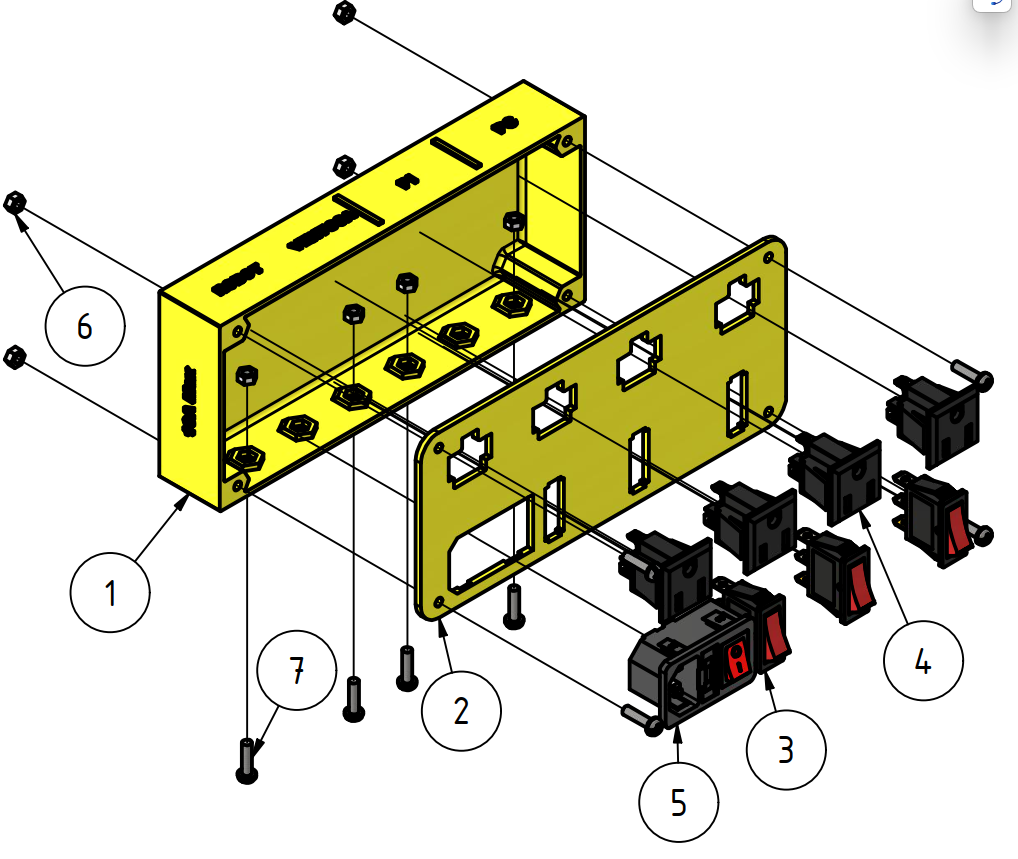
\includegraphics[width=0.85\textwidth]{06disenoConceptual/img/multitoma/multitoma.png}
    \caption{Ensamble explosionado de la multitoma personalizada. (1) Carcasa fabricada en PETG mediante FDM, incorpora cavidades para tuercas M4 cautivas en base. (2) Tapa de la multitoma con perforaciones para montaje de componentes eléctricos. (3) Switches balancín KCD3 de 3 pines con piloto LED integrado (3 unidades). (4) Tomas de corriente AC 125V/15A para montaje en panel (4 unidades). (5) Conector de entrada AC-01 para cable C13 con switch maestro y portafusible integrado. (6) Tuercas M4 cautivas para anclaje a plataforma (8 unidades). (7) Tornillos M4 × 15 mm para unión tapa-carcasa (8 unidades).}
    \label{fig:multitoma}
\end{figure}

\begin{table}[H]
\centering
\caption{Lista de materiales de la multitoma personalizada}
\label{tab:bom_multitoma}
\small
\begin{tabular}{|c|l|c|l|l|}
\hline
\textbf{\#} & \textbf{Componente} & \textbf{Cant.} & \textbf{Fabricación} & \textbf{Material} \\
\hline
1 & Carcasa de multitoma & 1 & FDM & PETG \\
2 & Tapa de multitoma & 1 & FDM & PETG \\
3 & Switch balancín KCD3 3 pines con piloto & 3 & Comercial & --- \\
4 & Toma AC 125V/15A montaje panel & 4 & Comercial & --- \\
5 & Conector entrada AC-01 cable C13 & 1 & Comercial & --- \\
6 & Tuerca M4 & 8 & Comercial & Acero \\
7 & Tornillo M4 × 15 mm & 8 & Comercial & Acero \\
8 & Fusible 15A 125V AC cartucho & 1 & Comercial & --- \\
9 & Cable cobre 14 AWG rojo × 1 m & 1 & Comercial & Cobre \\
10 & Cable cobre 14 AWG verde × 1 m & 1 & Comercial & Cobre \\
11 & Cable cobre 14 AWG blanco × 1 m & 1 & Comercial & Cobre \\
12 & Cable de poder C13 × 2 m & 1 & Comercial & --- \\
\hline
\end{tabular}
\end{table}

\textit{Nota: Los componentes 8-12 (cableado y fusible) no se representan en la Figura \ref{fig:multitoma} pues no eran necesarios para visualización del ensamblaje mecánico en modelo 3D.}

\subsubsection{Arquitectura de Ensamblaje}

El diseño de la multitoma emplea arquitectura de dos piezas principales:

\paragraph{Carcasa Base}

\begin{itemize}
    \item Fabricada en PETG por resistencia mecánica superior a PLA y menor deformación térmica
    \item Color amarillo para alta visibilidad de advertencias de seguridad
    \item Cavidades hexagonales en base inferior para alojar tuercas M4 cautivas
    \item Marquillas en relieve en superficie superior indicando posición de cada fuente
    \item Rebajes laterales para paso de cables de alimentación
\end{itemize}

\paragraph{Tapa con Componentes Eléctricos}

\begin{itemize}
    \item Todos los componentes eléctricos (switches, tomas, conector de entrada) se montan en la tapa
    \item Perforaciones dimensionadas para ajuste apretado de tomas AC (previene rotación)
    \item Cableado interno se realiza en tapa antes de cierre final
    \item Tapa se atornilla a carcasa mediante 8 tornillos M4 × 15 mm perimetrales
\end{itemize}

Esta arquitectura permite:
\begin{itemize}
    \item Ensamblaje y cableado de componentes eléctricos con carcasa abierta (acceso superior completo)
    \item Inspección visual de conexiones antes de cierre
    \item Mantenimiento o reemplazo de componentes sin desmontar multitoma de la plataforma
    \item Pruebas eléctricas previas al ensamblaje final
\end{itemize}

\paragraph{Anclaje a Plataforma Base}

Las tuercas M4 cautivas en la base de la carcasa permiten atornillar la multitoma a la plataforma MDF mediante tornillos que atraviesan desde la cara inferior de la plataforma. Esta configuración:
\begin{itemize}
    \item Integra mecánicamente la multitoma al kit
    \item Previene movimiento durante conexión/desconexión de fuentes
    \item Facilita gestión de cables entre multitoma y componentes
    \item Permite desmontaje completo para mantenimiento mayor
\end{itemize}

\subsection{Conclusión}

El diseño de la multitoma personalizada resuelve las limitaciones de soluciones comerciales mediante espaciamiento optimizado para fuentes de geometrías variables, control individual de energización de subsistemas con identificación clara, protección eléctrica mediante fusible accesible, y cumplimiento normativo RETIE en cableado interno. La arquitectura modular tapa-carcasa facilita ensamblaje, inspección y mantenimiento, mientras que la integración mecánica a la plataforma base proporciona estabilidad operativa y gestión ordenada de alimentación eléctrica del kit educativo.
\section{Kit de Clasificación Completo}

La integración de todos los subsistemas diseñados (mecánico, neumático, de control, de visión y eléctrico) resulta en un kit educativo compacto y funcional para enseñanza de robótica, visión por computador y ROS2. La Figura \ref{fig:kitCompleto} presenta el ensamblaje completo del kit con todos sus componentes principales.

\begin{figure}[H]
    \centering
    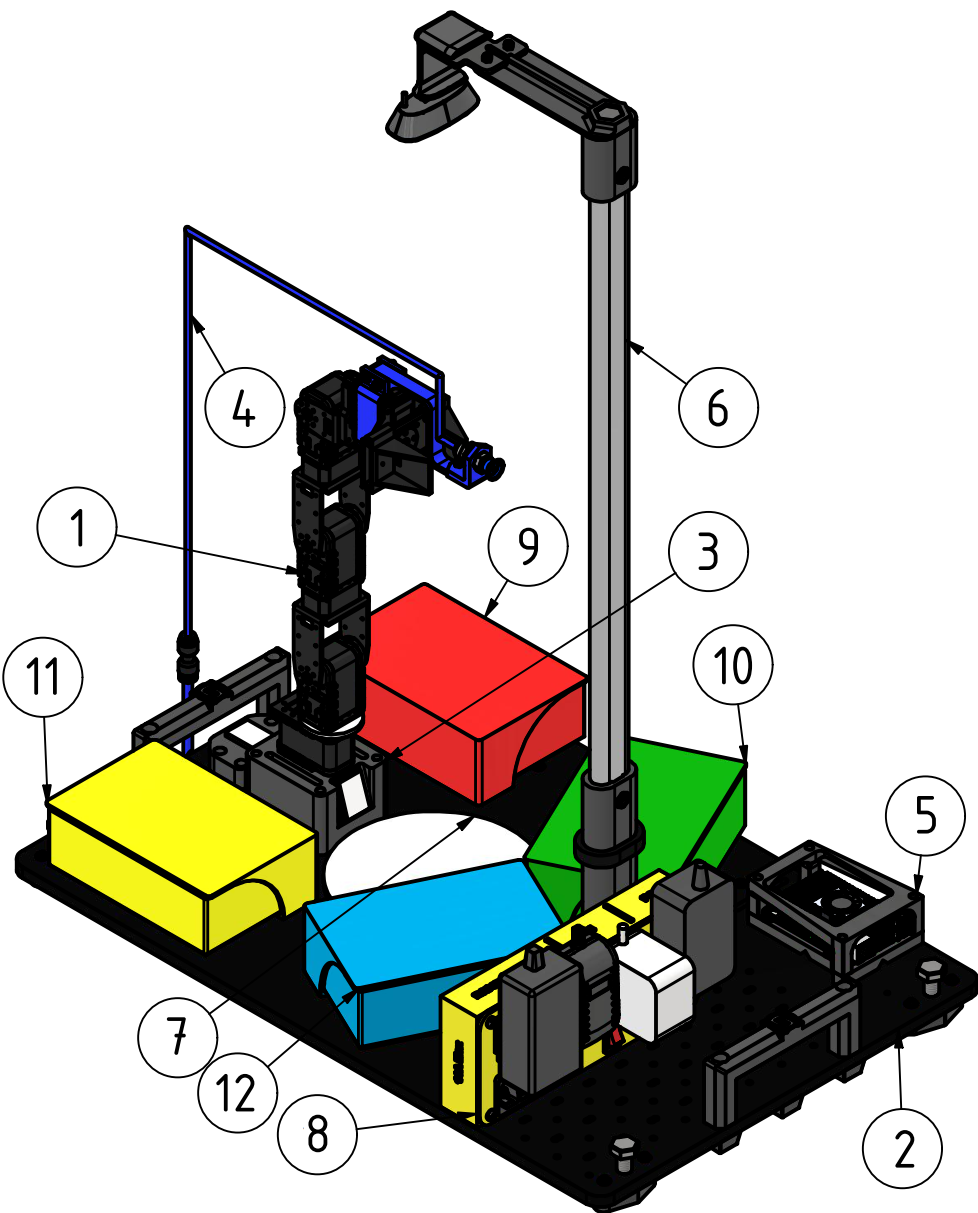
\includegraphics[width=0.9\textwidth]{06disenoConceptual/img/kit.png}
    \caption{Kit de clasificación completo ensamblado. (1) Manipulador robótico PhantomX Pincher AX-12 con 4 grados de libertad, (2) Plataforma base de MDF (554 mm × 360 mm × 9 mm) con acabado negro mate, (3) Base del manipulador con sistema de identificación numérica, (4) Sistema de succión por vacío con gripper intercambiable, (5) Controlador Raspberry Pi 5 en carcasa protectora, (6) Soporte de cámara con mástil vertical y brazo en voladizo, (7) Zona de recolección circular blanca (Ø146 mm), (8) Multitoma personalizada con control individual de subsistemas, (9) Caneca de depósito roja, (10) Caneca de depósito verde, (11) Caneca de depósito azul, (12) Caneca de depósito amarilla. Todos los componentes se integran en contenedor plástico de 600 mm × 400 mm para almacenamiento y transporte.}
    \label{fig:kitCompleto}
\end{figure}

\subsection{Componentes Principales del Kit}

El kit integrado está compuesto por los siguientes subsistemas y componentes principales:

\begin{table}[H]
\centering
\caption{Componentes principales del kit de clasificación}
\label{tab:componentes_kit}
\small
\begin{tabular}{|c|l|}
\hline
\textbf{\#} & \textbf{Componente/Subsistema} \\
\hline
1 & Manipulador PhantomX Pincher AX-12 \\
2 & Plataforma base \\
3 & Base de manipulador \\
4 & Sistema de succión por vacío \\
5 & Controlador (Raspberry Pi 5) \\
6 & Soporte de cámara \\
7 & Zona de recolección \\
8 & Multitoma personalizada \\
9 & Caneca de depósito roja \\
10 & Caneca de depósito verde \\
11 & Caneca de depósito azul \\
12 & Caneca de depósito amarilla \\
\hline
\end{tabular}
\end{table}

\subsection{Características Generales del Kit}

El kit completo presenta las siguientes características técnicas y operativas:

\subsubsection{Dimensiones y Peso}

\begin{itemize}
    \item \textbf{Plataforma operativa}: 554 mm × 360 mm × 706 mm (largo × ancho × alto máximo con soporte de cámara)
    \item \textbf{Contenedor de almacenamiento}: 600 mm × 400 mm × 171 mm (exteriores)
    \item \textbf{Peso total estimado}: 4.5-5.5 kg (incluye todos los componentes y objetos de clasificación)
    \item \textbf{Portabilidad}: Transporte manual mediante asas integradas en contenedor
\end{itemize}

\subsubsection{Capacidades Funcionales}

\begin{itemize}
    \item \textbf{Espacio de trabajo}: Zona de recolección de Ø146 mm más cuatro zonas de depósito
    \item \textbf{Capacidad de manipulación}: Objetos de 25 mm × 25 mm × 25 mm, peso máximo 30 g
    \item \textbf{Tipos de objetos}: 4 geometrías distinguibles (cuadrado, rectángulo, círculo, pentágono)
    \item \textbf{Modos de operación}: Gripper mecánico o sistema de succión por vacío (intercambiables)
    \item \textbf{Clasificación por color}: 4 categorías (rojo, verde, azul, amarillo)
\end{itemize}

\subsubsection{Subsistemas Integrados}

\begin{itemize}
    \item \textbf{Subsistema mecánico}: Manipulador de 4 DOF, plataforma estructural, zonas de trabajo
    \item \textbf{Subsistema neumático}: Bomba de vacío 370A, ventosa PAK-15, mangueras de 4-6 mm
    \item \textbf{Subsistema de control}: Raspberry Pi 5 (8 GB RAM), Ubuntu 24.04 LTS, ROS2 Jazzy
    \item \textbf{Subsistema de visión}: Cámara Logitech C270, soporte ajustable en altura
    \item \textbf{Subsistema eléctrico}: Multitoma con 4 salidas, 3 switches individuales, protección por fusible 15A
\end{itemize}

\subsubsection{Recursos Didácticos}

El kit proporciona plataforma para práctica de:

\begin{itemize}
    \item Cinemática directa e inversa de manipuladores seriales
    \item Control de servomotores Dynamixel mediante protocolos de comunicación
    \item Visión por computador (segmentación de color, detección de formas, calibración de cámara)
    \item Programación de nodos ROS2 en Python/C++
    \item Planificación de trayectorias y evasión de colisiones
    \item Integración de sensores y actuadores en sistemas robóticos
    \item Desarrollo de interfaces de usuario para control de robots
\end{itemize}

\subsection{Configuración de Almacenamiento}

Todos los componentes del kit se almacenan en el contenedor plástico sellado mediante la siguiente distribución:

\begin{itemize}
    \item \textbf{Nivel inferior}: Plataforma base con canecas, zona de recolección, multitoma y base de manipulador fijos
    \item \textbf{Nivel medio}: Manipulador desmontado, carcasa de Raspberry Pi, bomba de vacío
    \item \textbf{Nivel superior}: Mástil de soporte de cámara (diagonal), gripper de succión, objetos de clasificación, cableado
    \item \textbf{Compartimentos laterales}: Fuentes de alimentación, cable de poder, mangueras neumáticas
\end{itemize}

Las tapas deslizantes de las canecas se cierran durante almacenamiento, conteniendo objetos de clasificación y previendo su pérdida durante transporte.
